\باب{طاقتی تسلسل سے سادہ تفرقی مساوات کا حل۔اعلٰی تفاعل}\شناخت{باب_بیسل}
گزشتہ ابواب میں \ترچھا{مستقل عددی سر} والے خطی سادہ تفرقی مساوات کے حل حاصل کیے گئے جو \اصطلاح{بنیادی تفاعل} تھے۔بنیاد تفاعل مثلاً \عددی{\sin 3t}، \عددی{t^6} اور \عددی{e^{2t}} کو آپ \اصطلاح{علم الاحصاء}\فرہنگ{علم الاحصاء}\حاشیہب{calculus}\فرہنگ{calculus} سے جانتے ہیں۔\اصطلاح{متغیر عددی سر} والے سادہ تفرقی مساوات کے حل نسبتاً مشکل سے حاصل ہوتے ہیں اور یہ حل غیر بنیادی تفاعل ہو سکتے ہیں۔ \اصطلاح{لیژانڈر}، \اصطلاح{بیسل} اور \اصطلاح{بیش ہندسی} مساوات اس نوعیت کے سادہ تفرقی مساوات ہیں۔یہ مساوات اور ان کے حل \اصطلاح{لیژانڈر تفاعل}، \اصطلاح{بیسل تفاعل} اور \اصطلاح{بیش ہندسی تفاعل} انجینئری میں نہایت اہم کردار ادا کرتے ہیں لہٰذا ان مساوات کو حل کرنے کے دو مختلف ترکیبوں پر غور کیا جائے گا۔

پہلی ترکیب میں مساوات کا حل \اصطلاح{طاقتی تسلسل}\فرہنگ{تسلسل!طاقتی}\فرہنگ{طاقتی!تسلسل}\حاشیہب{power series}\فرہنگ{series!power}\فرہنگ{power series} \عددی{a_0+a_1x+a_2x^2+a_3x^3+\cdots} کی صورت میں حاصل کیا جاتا ہے لہٰذا اس کو \اصطلاح{ترکیب طاقتی تسلسل}\فرہنگ{ترکیب طاقتی تسلسل}\فرہنگ{طاقتی تسلسل!ترکیب}\حاشیہب{power series method}\فرہنگ{power series method} کہتے ہیں۔

طاقتی تسلسل کو \عددی{\ln x} یا کسری طاقت \عددی{x^r} سے ضرب دیتے ہوئے دوسری ترکیب حاصل ہوتی ہے جو \اصطلاح{ترکیب فروبنیوس}\فرہنگ{ترکیب فروبنیوس}\فرہنگ{فروبنیوس!ترکیب}\حاشیہب{Frobenius method}\فرہنگ{Frobenius method} کہلاتی ہے۔جہاں خالصتاً طاقتی تسلسل کی صورت میں حل لکھنا ممکن نہ ہو وہاں ترکیب فروبنیوس کار آمد ثابت ہوتا ہے لہٰذا یہ ترکیب زیادہ عمومی ہے۔

ایسے تمام اعلٰی حل جنہیں آپ علم الاحصاء سے نہیں جانتے  \اصطلاح{اعلٰی تفاعل}\فرہنگ{اعلٰی تفاعل}\حاشیہب{higher functions or special functions}\فرہنگ{higher functons}\فرہنگ{special functions} کہلاتے ہیں۔
%================

\حصہ{ترکیب طاقتی تسلسل}\شناخت{حصہ_ترکیب_طاقتی_تسلسل}
\موٹا{متغیر} عددی سر والے خطی سادہ تفرقی مساوات کو عموماً \اصطلاح{ترکیب طاقتی تسلسل} سے حل کرتے ہوئے طاقتی تسلسل کی صورت میں حل حاصل کیا جاتا ہے۔اس طاقتی تسلسل سے حل کی قیمت دریافت کی جا سکتی ہے، حل کا خط کھینچا جا سکتا ہے، کلیات ثابت کیے جا سکتے ہیں اور اسی طرح دیگر معلومات حاصل کی جا سکتی ہے۔اس حصے میں طاقتی تسلسل کے تصور پر غور کیا جائے گا۔

علم الاحصاء سے ہم جانتے ہیں کہ \عددی{x-x_0} کا طاقتی تسلسل درج ذیل ہے
\begin{align}\label{مساوات_بیسل_تسلسل_الف} 
\sum_{m=0}^{\infty} a_m(x-x_0)^m=a_0+a_1(x-x_0)+a_2(x-x_0)^2+a_3(x-x_0)^3+\cdots
\end{align}
جس میں \عددی{x} متغیر ہے جبکہ \عددی{a_0}،\عددی{a_1}،\عددی{a_2}،\نقطے تسلسل کے \اصطلاح{عددی سر}\فرہنگ{عددی سر}\حاشیہب{coefficients}\فرہنگ{coefficients} کہلاتے ہیں اور \عددی{x_0} مستقل مقدار ہے جو تسلسل کا \اصطلاح{وسط}\فرہنگ{وسط}\حاشیہب{center}\فرہنگ{center} کہلاتا ہے۔جیسا مساوات \حوالہ{مساوات_بیسل_تسلسل_الف} میں دکھایا گیا ہے، تسلسل کو عموماً \اصطلاح{علامت مجموعہ}\فرہنگ{علامت مجموعہ}\حاشیہب{summation}\فرہنگ{summation} (\عددی{\sum}) کی مدد سے مختصراً لکھا جاتا ہے جس میں \اصطلاح{اشاریہ}\فرہنگ{اشاریہ}\حاشیہب{index}\فرہنگ{index} مختلف اجزاء کی نشاندہی کرتی ہے۔درج بالا مساوات میں \عددی{m} بطور اشاریہ استعمال کیا گیا ہے۔علامت مجموعہ کے نیچے \عددی{m=0} اور اس کے اوپر \عددی{\infty} مجموعے کی پہلے اور آخری جزو کی نشاندہی کرتے ہیں۔  تسلسل کا وسط صفر \عددی{(x_0=0)} ہونے کی صورت میں \عددی{x} کا طاقتی تسلسل
\begin{align} \label{مساوات_بیسل_تسلسل_ب} 
\sum_{m=0}^{\infty} a_m x^m=a_0+a_1 x+a_2 x^2+a_3 x^3+\cdots
\end{align}
 حاصل ہوتا ہے۔ہم فرض کرتے ہیں کہ تمام متغیرات اور مستقل مقدار \موٹا{حقیقی} ہے۔

طاقتی تسلسل سے مراد مساوات \حوالہ{مساوات_بیسل_تسلسل_الف} یا مساوات \حوالہ{مساوات_بیسل_تسلسل_ب} کی تسلسل ہے جس میں \عددی{x-x_0} (یا \عددی{x}) کا منفی طاقت یا کسری طاقت \موٹا{نہیں} پایا جاتا۔
%=============

\ابتدا{مثال}\quad \اصطلاح{مکلارن} تسلسل درحقیقت میں طاقتی تسلسل ہیں\\
\begin{align*}
\frac{1}{1-x}&=\sum_{m=0}^{\infty}x^m=1+x+x^2+x^3+\cdots\quad \quad (\abs{x}<1,\, \text{\RL{ہندسی تسلسل}})\\
e^x&=\sum_{m=0}^{\infty} \frac{x^m}{m!}=1+x+\frac{x^2}{2!}+\frac{x^3}{3!}+\cdots\\
\sin x&=\sum_{m=0}^{\infty} \frac{(-1)^m x^{2m+1}}{(2m+1)!}=x-\frac{x^3}{3!}+\frac{x^5}{5!}-+\cdots\\
\cos x&=\sum_{m=0}^{\infty}\frac{(-1)^m x^{2m}}{(2m)!}=1-\frac{x^2}{2!}+\frac{x^4}{4!}-+\cdots
\end{align*}
\انتہا{مثال}
%======================

\جزوحصہء{ترکیب طاقتی تسلسل کا تصور}
آپ نے درج بالا مثال میں کئی بنیادی تفاعل کے طاقتی تسلسل دیکھے۔یوں آپ دیکھ سکتے ہیں کہ خطی سادہ تفرقی مساوات کا حل طاقتی تسلسل کی صورت میں لکھا جا سکتا ہے۔ ایک مثال کی مدد سے اس ترکیب کو سمجھتے ہیں۔
%===========

\ابتدا{مثال}\quad طاقتی تسلسل حل \\
تفرقی مساوات \عددی{y'+y=0} کو ترکیب طاقتی تسلسل سے حل کریں۔

حل:پہلی قدم میں حل کو طاقتی تسلسل کی صورت میں لکھ کر
\begin{align}\label{مساوات_بیسل_طاقتی_تسلسل_حل_الف}
y=a_0+a_1x+a_2x^2+a_3x^3+\cdots=\sum_{m=0}^{\infty} a_m x^m
\end{align}
تسلسل کا جزو با جزو تفرق لیتے ہیں۔
\begin{align}\label{مساوات_بیسل_طاقتی_تسلسل_حل_ب}
y'=a_1+2a_2x+3a_3x^2+\cdots=\sum_{m=1}^{\infty} ma_mx^{m-1}
\end{align}
انہیں دیے گئے تفرقی مساوات میں پر کرتے ہوئے
\begin{align*}
(a_0+a_1x+a_2x^2+a_3x^3+\cdots)+(a_1+2a_2x+3a_3x^2+\cdots)=0
\end{align*}
\عددی{x} کی طاقت کے لحاظ سے ترتیب دیتے ہیں۔
\begin{align*}
(a_0+a_1)+(a_1+2a_2)x+(a_2+3a_3)x^2+\cdots=0
\end{align*}
اس مساوات کا دایاں ہاتھ صفر کے برابر ہے لہٰذا بائیں ہاتھ تمام اجزاء بھی صفر کے برابر ہوں گے۔
\begin{align*}
a_0+a_1=0,\quad a_1+2a_2=0, \quad a_2+3a_3=0
\end{align*}
ان سے درج ذیل لکھا جا سکتا ہے۔
\begin{align*}
a_1=-a_0,\quad a_2=-\frac{a_1}{2}=\frac{a_0}{2},\quad a_3=-\frac{a_2}{3}=-\frac{a_0}{3!}
\end{align*}
ان عددی سر کو استعمال کرتے ہوئے  حل \حوالہ{مساوات_بیسل_طاقتی_تسلسل_حل_الف} لکھتے ہیں جو قوت نمائی تفاعل \عددی{e^{-x}} کی مکلارن تسلسل ہے۔
\begin{align*}
y=a_0(1-x+\frac{x^2}{2!}-\frac{x^3}{3!}+-\cdots)=a_0 e^{-x}
\end{align*}
یہاں آپ  \عددی{y''+y=0} کو ترکیب طاقتی تسلسل سے حل کرتے ہوئے حل \عددی{y=a_0\cos x+a_1\sin x} حاصل کریں۔
\انتہا{مثال}
%=================

اب اس ترکیب کی عمومی استعمال پر غور کرتے ہیں جبکہ اگلے مثال کے بعد اس کا جواز پیش کرتے ہیں۔پہلی قدم میں ہم خطی سادہ تفرقی مساوات
\begin{align}\label{مساوات_بیسل_طاقتی_عمومی_مساوات_الف}
y''+p(x)y'+q(x)y=0
\end{align}
میں \عددی{p(x)} اور \عددی{q(x)} کو \عددی{x} کے تسلسل کی صورت  (اور اگر حل \عددی{x-x_0} کی تسلسل کی صورت میں درکار ہو تب انہیں \عددی{x-x_0} کی تسلسل کی صورت) میں لکھتے ہیں۔ اگر \عددی{p(x)} اور \عددی{q(x)} اذ خود  \ترچھا{کثیر رکنی}  ہوں تب پہلی قدم میں کچھ کرنے کی ضرورت نہیں ہے۔ دوسری قدم میں حل کو مساوات \حوالہ{مساوات_بیسل_طاقتی_تسلسل_حل_الف} کی طرح تصور کرتے ہوئے  مساوات \حوالہ{مساوات_بیسل_طاقتی_تسلسل_حل_ب} کی طرح \عددی{y'} اور درج ذیل \عددی{y''} لکھتے ہوئے
\begin{align}\label{مساوات_بیسل_طاقتی_تسلسل_حل_پ}
y''=2a_2+3\cdot 2 a_3x+4\cdot 3 a_4x^2+5\cdot 4 a_5 x^3+\cdots=\sum_{m=2}^{\infty} m(m-1)a_mx^{m-2}
\end{align}
مساوات \حوالہ{مساوات_بیسل_طاقتی_عمومی_مساوات_الف} میں پر کریں۔تیسری قدم میں \عددی{x} کی طاقت کے لحاظ سے ترتیب دیتے ہوئے، مستقل مقدار سے شروع کرتے ہوئے، باری باری \عددی{x^1}، \عددی{x^2}، \نقطے کے عددی سر کو صفر کے برابر پر کریں۔یوں تمام عددی سر کو \عددی{a_0} اور \عددی{a_1} کی صورت میں حاصل کرتے ہوئے اصل حل لکھیں۔
%===============

\ابتدا{مثال}\شناخت{مثال_بیسل_کلیہ_توالی_الف} \quad ایک مخصوص \اصطلاح{لیژانڈر مساوات}\\
درج ذیل مساوات کروی تشاکل خاصیت رکھتی ہے۔اس کو حل کریں۔
\begin{align*}
(1-x^2)y''-2xy'+2y=0
\end{align*} 
حل:مساوات \حوالہ{مساوات_بیسل_طاقتی_تسلسل_حل_الف}، مساوات \حوالہ{مساوات_بیسل_طاقتی_تسلسل_حل_ب} اور مساوات \حوالہ{مساوات_بیسل_طاقتی_تسلسل_حل_پ} کو درج بالا میں پر کرتے ہوئے
\begin{multline*}
(1-x^2)(2a_2+3\cdot 2 a_3x+4\cdot 3 a_4x^2+5\cdot 4 a_5x^3+6\cdot 5 a_6x^4\cdots)\\
-2x(a_1+2a_2x+3a_3x^2+4a_4x^3+\cdots)\\
+2(a_0+a_1x+a_2x^2+a_3x^3+a_4x^4+\cdots)=0
\end{multline*}
یعنی
\begin{multline*}
(2a_2+3\cdot 2 a_3x+4\cdot 3 a_4x^2+5\cdot 4a_5 x^3+6\cdot 5 a_6x^4\cdots)\\
+(-2a_2 x^2-3\cdot 2 a_3x^3-4\cdot 3a_4 x^4-5\cdot 4a_5x^5-\cdots)\\
+(-2a_1x-2\cdot 2a_2x^2-3\cdot 2a_3x^3-4\cdot 2 a_4x^4-\cdots)\\
+(2a_0+2a_1x+2a_2x^2+2a_3x^3+2a_4x^4+\cdots)=0
\end{multline*}
ملتا ہے جس کو \عددی{x} کی طاقت کے لحاظ سے ترتیب دیتے ہیں۔
\begin{multline*}
(2a_2+2a_0)+(3\cdot 2 a_3-2a_1+2a_1)x\\
+(4\cdot 3 a_4-2a_2-2\cdot 2a_2+2a_2)x^2\\
+(5\cdot 4a_5-3\cdot 2 a_3-3\cdot 2a_3+2a_3)x^3\\
+(6\cdot 5a_6-4\cdot 3a_4-4\cdot 2a_4+2a_4)x^4+\cdots=0
\end{multline*}
مستقل مقدار سے شروع کرتے ہوئے باری باری \عددی{x}، \عددی{x^2}، \عددی{x^3}، \نقطے کے عددی سر کو صفر کے برابر پر کرتے ہوئے بالترتیب \عددی{a_2}،\عددی{a_3}،\عددی{a_4}، \نقطے کو \عددی{a_0} اور \عددی{a_1} کی صورت میں حاصل کرتے ہیں۔
\begin{align*}
a_2&=-a_0\\
a_3&=0\\
a_4&=\frac{a_2}{3}=-\frac{a_0}{3}\\
a_5&=\frac{a_3}{2}=0\quad \text{\RL{(چونکہ \عددی{a_3=0} ہے)}}\\
a_6&=\frac{3}{5}a_4=-\frac{a_0}{5}
\end{align*}
ان عددی سروں کو مساوات \حوالہ{مساوات_بیسل_طاقتی_تسلسل_حل_الف} میں پر کرتے ہوئے حل لکھتے ہیں
\begin{align*}
y=a_1x+a_0(1-x^2-\frac{1}{3}x^4-\frac{1}{5}x^6-\cdots)
\end{align*}
جس میں \عددی{a_0} اور \عددی{a_1} اختیاری مستقل ہیں۔یوں درج بالا عمومی حل دو عدد حل \عددی{x} اور \عددی{1-x^2-\tfrac{1}{3}x^4-\cdots} پر مشتمل ہے جو  \اصطلاح{لیژانڈر کثیر رکنی}\فرہنگ{لیژانڈر!کثیر رکنی تفاعل}\حاشیہب{Legendre polynomials}\فرہنگ{Legendre!polynomial} \عددی{P_n(x)} اور \اصطلاح{لیژانڈر تفاعل}\فرہنگ{لیژانڈر!تفاعل}\حاشیہب{Legendre function}\فرہنگ{Legendre!function} \عددی{Q_n(x)} کے رکن  ہیں۔یہاں \عددی{x=P_1(x)} اور 
\عددی{1-x^2-\frac{1}{3}x^4-\frac{1}{5}x^6-\cdots=-Q_1(x)} ہیں جہاں منفی علامت روایتی ہے۔\عددی{n} لیژانڈر کثیر رکنی اور لیژانڈر تفاعل کا \اصطلاح{درجہ}\فرہنگ{درجہ!لیژانڈر}\حاشیہب{order}\فرہنگ{order!Legendre} کہلاتا ہے۔یہاں \عددی{n=1} ہے لہٰذا لیژانڈر کثیر رکنی اور لیژانڈر تفاعل کا درجہ \عددی{1} ہے۔
\انتہا{مثال}
%===================

\جزوحصہء{نظریہ طاقتی تسلسل}
مساوات \حوالہ{مساوات_بیسل_تسلسل_الف} کے چند ارکان کا جزوی مجموعہ \عددی{s_n(x)} لکھتے ہیں جس کو \عددی{n} \اصطلاح{جزوی مجموعہ}\فرہنگ{جزوی مجموعہ}\حاشیہب{nth partial sum}\فرہنگ{partial sum} کہتے ہیں۔ 
\begin{align}
s_n(x)=a_0+a_1(x-x_0)+a_2(x-x_0)^2+\cdots +a_n (x-x_0)^n
\end{align}
یہاں \عددی{n=0,1,2,\cdots} ممکن ہے۔مساوات \حوالہ{مساوات_بیسل_تسلسل_الف} سے \عددی{s_n(x)} منفی کرنے سے بقایا \عددی{R_n(x)} حاصل ہوتا ہے جس کو \عددی{a_n(x-x_0)^n} کے بعد  مساوات \حوالہ{مساوات_بیسل_تسلسل_الف} کا \اصطلاح{بقایا}\فرہنگ{بقایا}\حاشیہب{remainder}\فرہنگ{remainder} کہتے ہیں۔
\begin{align}
R_n(x)=a_{n+1}(x-x_0)^{n+1}+a_{n+2}(x-x_0)^{n+2}+\cdots
\end{align}
یوں ہندسی تسلسل 
\begin{align*}
1+x+x^2+x^3+x^4+\cdots
\end{align*}
کے \اصطلاح{جزوی مجموعے} اور نظیری \اصطلاح{بقایا} درج ذیل ہوں گے۔
\begin{align*}
s_0&=1, &R_0=x+x^2+x^3+\cdots\\
s_1&=1+x,&R_1=x^2+x^3+x^4+\cdots\\
s_2&=1+x+x^2, &R_2=x^3+x^4+x^5+\cdots
\end{align*}
اس طرح مساوات \حوالہ{مساوات_بیسل_تسلسل_الف} کے ساتھ ہم جزوی مجموعوں \عددی{s_0(x)}، \عددی{s_1(x)}،\عددی{s_2(x)} \نقطے کی ترتیب وابستہ کرتے ہیں۔اگر کسی \عددی{x=x_1} کے لئے جزوی مجموعوں کی ترتیب  مرتکز ہو مثلاً 
\begin{align*}
\lim_{n \to \infty} s_n(x_1)=s(x_1)
\end{align*}
تب  ہم کہتے ہیں کہ نقطہ \عددی{x=x_1} پر تسلسل \حوالہ{مساوات_بیسل_تسلسل_الف} \اصطلاح{مرکوز}\فرہنگ{مرتکز}\حاشیہب{converge}\فرہنگ{converge} ہے جبکہ \عددی{s(x_1)} کو تسلسل \حوالہ{مساوات_بیسل_تسلسل_الف} کی \اصطلاح{قیمت}\فرہنگ{طاقتی تسلسل!قیمت}\حاشیہب{value or sum}\فرہنگ{power series!value or sum} یا \اصطلاح{مجموعہ}\فرہنگ{طاقتی تسلسل!مجموعہ} کہتے ہیں جس کو درج ذیل لکھا جاتا ہے۔
\begin{align*}
s(x_1)=\sum_{m=0}^{\infty} a_m(x_1-x_0)^m
\end{align*}
اس طرح کسی بھی \عددی{n} کے لئے ہم درج ذیل لکھ سکتے  ہیں۔
\begin{align}\label{مساوات_بیسل_تسلسل_مجموعہ_الف}
s(x_1)=s_n(x_1)+R_n(x_1)
\end{align}
اس کے برعکس اگر \عددی{s_0(x)}، \عددی{s_1(x)}، \عددی{s_2(x)}، \نقطے کی ترتیب غیر مرکوز ہو تب ہم کہتے ہیں کہ نقطہ \عددی{x=x_1} پر مساوات \حوالہ{مساوات_بیسل_تسلسل_الف} \اصطلاح{منفرج}\فرہنگ{منفرج}\حاشیہب{divergent}\فرہنگ{divergent} ہے۔

مرکوز تسلسل کی صورت میں، کسی بھی مثبت \عددی{\epsilon} کے لئے  ایسا \عددی{N} (جس کی قیمت \عددی{\epsilon} پر منحصر ہے) پایا جاتا ہے کہ ہم تمام \عددی{n>N} کے لئے   مساوات \حوالہ{مساوات_بیسل_تسلسل_مجموعہ_الف} سے درج ذیل لکھ سکتے ہیں۔ 
\begin{align}\label{مساوات_بیسل_مرتکز_حدود}
\abs{R_n(x_1)}=\abs{s(x_1)-s_n(x_1)} < \epsilon \quad \quad \text{\RL{تمام \عددی{n>N}}}
\end{align}
جیومیٹریائی طور (شکل \حوالہ{شکل_مساوات_بیسل_مرتکز_حدود} دیکھیں) پر اس کا مطلب ہے کہ \عددی{s_n(x_1)} جہاں \عددی{n>N} ہے \عددی{s(x_1)-\epsilon} اور \عددی{s(x_1)+\epsilon} کے درمیان پایا جاتا ہے۔عملاً اس کا مطلب ہے کہ مرکوز تسلسل کی صورت  میں \عددی{x_1} پر  مساوات \حوالہ{مساوات_بیسل_تسلسل_الف} کا مجموعہ \عددی{s(x_1)} تقریباً \عددی{s_n(x_1)} کے برابر ہو گا۔مزید یہ کہ \عددی{s(x_1)} اور \عددی{s_n(x_1)} میں فرق کو ہم \عددی{n} بڑھا کر جتنا کم بنانا چاہیں بنا سکتے ہیں۔
\begin{figure}
\centering
\begin{tikzpicture}
\draw(-\x-\x/2,0)--(\x+\x/2,0);
\draw(-\x,-\y/16)node[below]{$s(x_1)-\epsilon$}--++(0,\y/8)coordinate (kL);
\draw(0,-\y/16)node[below]{$s(x_1)$}--++(0,\y/8)coordinate(kM);
\draw(\x,-\y/16)node[below]{$s(x_1)+\epsilon$}--++(0,\y/8)coordinate (kR);
\draw[gray] (kL)++(0,\y/16)--++(0,\y/8)coordinate[pos=0.5](kLA);
\draw[gray] (kM)++(0,\y/16)--++(0,\y/8)coordinate[pos=0.5](kMA);
\draw[gray] (kR)++(0,\y/16)--++(0,\y/8);
\draw[stealth-stealth] (kLA)--++(\x,0)node[pos=0.5,fill=white]{$\epsilon$};
\draw[stealth-stealth] (kMA)--++(\x,0)node[pos=0.5,fill=white]{$\epsilon$};
\end{tikzpicture}
\caption{غیر مساوات \حوالہ{مساوات_بیسل_مرتکز_حدود} کی شکل۔}
\label{شکل_مساوات_بیسل_مرتکز_حدود}
\end{figure}

طاقتی تسلسل کہاں مرکوز ہوتی ہے؟ تسلسل \حوالہ{مساوات_بیسل_تسلسل_الف} میں \عددی{x=x_0} پر  \عددی{a_0} کے علاوہ تمام اجزاء صفر ہو جاتے ہیں لہٰذا تسلسل کی قیمت \عددی{a_0} ہو گی۔یوں \عددی{x=x_0} پر تسلسل \عددی{a_0} پر مرکوز ہوتی ہے۔ کبھی کبھار \عددی{x} کی واحد اسی قیمت پر تسلسل مرتکز ہو گا۔ اگر \عددی{x} کے دیگر قیمتوں کے لئے بھی تسلسل مرتکز ہو تب \عددی{x} کی یہ قیمتیں \اصطلاح{ارتکازی وقفہ}\فرہنگ{ارتکازی وقفہ}\فرہنگ{وقفہ!ارتکازی}\حاشیہب{convergence interval}\فرہنگ{interval!convergence} کہلاتا ہے۔ یہ وقفہ محدود ہو سکتا ہے۔محدود وقفہ جس کا وسط \عددی{x_0} ہے کو شکل \حوالہ{شکل_مساوات_بیسل_مرتکز_محدود_وقفہ} میں دکھایا گیا ہے۔یوں طاقتی تسلسل \حوالہ{مساوات_بیسل_تسلسل_الف} ارتکازی وقفے کے اندر تمام \عددی{x} پر مرکوز ہو گا یعنی درج ذیل مساوات پر پورا اترنے والے \عددی{x} پر تسلسل مرکوز ہو گا
\begin{align}\label{مساوات_بیسل_ارتکازی_وقفہ}
\abs{x-x_0}<R
\end{align}
جبکہ \عددی{\abs{x-x_0}>R} پر تسلسل منفرج ہو گا۔ارتکازی وقفہ لامتناہی بھی ہو سکتا ہے اور ایسی صورت میں طاقتی تسلسل \عددی{x} کی تمام قیمتوں پر مرکوز ہو گا۔
\begin{figure}
\centering
\begin{tikzpicture}
\draw(-\x-\x/2,0)--(\x+\x/2,0);
\draw(-\x,-\y/16)node[below]{$x_0-R$}--++(0,\y/8)coordinate (kL);
\draw(0,-\y/16)node[below]{$x_0$}--++(0,\y/8)coordinate(kM);
\draw(\x,-\y/16)node[below]{$x_0+R$}--++(0,\y/8)coordinate (kR);
\draw[gray] (kL)++(0,\y/16)--++(0,\y/2)coordinate[pos=0.9](kL);
\draw[gray] (kM)++(0,\y/16)--++(0,\y/8)coordinate[pos=0.5](kMA);
\draw[gray] (kR)++(0,\y/16)--++(0,\y/2);
\draw[stealth-stealth] (kMA)--++(-\x,0)node[pos=0.5,fill=white]{$R$};
\draw[stealth-stealth] (kMA)--++(\x,0)node[pos=0.5,fill=white]{$R$};
\draw[stealth-stealth] (kL)node[left]{منفرج}--++(2*\x,0)node[pos=0.5,fill=white]{مرکوزیت}node[right]{منفرج};
\end{tikzpicture}
\caption{ارتکازی وقفہ \حوالہ{مساوات_بیسل_ارتکازی_وقفہ} جس کا وسط \عددی{x_0} ہے۔}
\label{شکل_مساوات_بیسل_مرتکز_محدود_وقفہ}
\end{figure}

شکل \حوالہ{شکل_مساوات_بیسل_مرتکز_محدود_وقفہ} میں \عددی{R} \اصطلاح{رداس ارتکاز}\فرہنگ{رداس!ارتکاز}\فرہنگ{ارتکاز!رداس}\حاشیہب{convergence radius}\فرہنگ{convergence!radius}\فرہنگ{radius!convergence} کہلاتا ہے۔(مخلوط طاقتی تسلسل کی صورت میں ارتکازی وقفہ گول ٹکیا ہوتا ہے جس کا رداس \عددی{R} ہو گا)۔ اگر تسلسل تمام \عددی{x} پر مرکوز ہو تب ہم \عددی{R = \infty} یعنی \عددی{\tfrac{1}{R}=0} لکھتے ہیں۔

رداس ارتکاز کی قیمت کو تسلسل کے عددی سر استعمال کرتے ہوئے  درج ذیل کلیات سے حاصل کیا جا سکتا ہے، پس شرط یہ ہے کہ ان کلیات میں حد (\عددی{\lim}) موجود اور غیر صفر ہو۔اگر یہ حد لامتناہی ہو تب تسلسل \حوالہ{مساوات_بیسل_تسلسل_الف} صرف وسط \عددی{x_0} پر مرکوز ہو گا۔
\begin{align}
R&=\frac{1}{\lim\limits_{m \to \infty} \sqrt[m]{\abs{a_m}}}\\
R&=\frac{1}{\lim\limits_{m \to \infty} \abs{\frac{a_{m+1}}{a_m}}}
\end{align}
%=====================
\ابتدا{مثال}\شناخت{مثال_بیسل_رداس_ارتکاز_الف}\quad رداس ارتکاز \عددی{\infty}، \عددی{1} اور \عددی{0}\\
تینوں تسلسل میں \عددی{m \to \infty} لیتے ہوئے رداس  ارتکاز  \عددی{R} دریافت کرتے ہیں۔
\begin{align*}
e^x=\sum_{m=0}^{\infty} \frac{x^m}{m!}=1+x+\frac{x^2}{2!}+\cdots,\quad \abs{\frac{a_{m+1}}{a_m}}=\frac{\frac{1}{(m+1)!}}{\frac{1}{m!}}=\frac{1}{m+1} \to 0, \quad R \to \infty\\
\frac{1}{1-x}=\sum_{m=0}^{\infty}x^m=1+x+x^2+\cdots,\quad \abs{\frac{a_{m+1}}{a_m}}=\abs{\frac{1}{1}}=1, \quad R=1\\
\sum_{m=0}^{\infty} m!x^m=1+x+2x^2+\cdots,\quad \abs{\frac{a_{m+1}}{a_m}}=\abs{\frac{(m+1)!}{m!}}=m+1 \to \infty,\quad R \to 0
\end{align*} 
لامتناہی رداس ارتکاس \عددی{R \to \infty} سب سے بہتر اور کارآمد صورت ہے جبکہ \عددی{R=0} بے کار صورت ہے۔عموماً تسلسل کا رداس ارتکاز محدود ہوتا ہے۔
\انتہا{مثال}
%======================

درج بالا مثال میں \عددی{\tfrac{1}{1-x}} کے طاقتی تسلسل کا رداس ارتکاز \عددی{R=1} حاصل ہوا جہاں تسلسل کا وسط \عددی{x_0=0} ہے۔مساوات \حوالہ{مساوات_بیسل_ارتکازی_وقفہ} کے تحت \عددی{\abs{x} <1} کے لئے طاقتی تسلسل تفاعل \عددی{\tfrac{1}{1-x}} کو ظاہر کرتی ہے۔آئیں اس حقیقت کو تفصیل سے دیکھیں۔نقطہ \عددی{x=0.2} پر تفاعل کی قیمت \عددی{\tfrac{1}{1-0.2}=1.25} ہے جبکہ اس کے تسلسل میں \عددی{x=0.2} پر کرتے ہوئے بتدریج ارکان کی تعداد بڑھاتے ہوئے مجموعہ حاصل کرتے ہیں۔
\begin{align*}
1&=1\quad \quad \text{\RL{ایک رکن}}\\
1+0.2&=1.2\\
1+0.2+0.2^2&=1.24\\
1+0.2+0.2^2+0.2^3&=1.248\\
1+0.2+0.2^2+0.2^3+0.2^4&=1.2496\quad \quad \text{\RL{پانچ ارکان}}
\end{align*}
طاقتی تسلسل کے پانچ ارکان کا مجموعہ تفاعل کے اصل قیمت کے \عددی{\tfrac{1.2496}{1.25}\times 100=99.968} فی صد ہے۔آپ دیکھ سکتے ہیں کہ، مجموعہ لیتے ہوئے  ارکان کی تعداد بڑھانے سے تسلسل کی قیمت اصل قیمت پر \اصطلاح{مرکوز} ہوتی ہے۔بالکل اسی طرح رداس ارتکاز کے اندر کسی بھی \عددی{x} پر تسلسل سے تفاعل کی قیمت، اصل قیمت کے قریب سے قریب تر، حاصل کی جا سکتی ہے۔

رداس ارتکاز کے باہر تسلسل منفرج ہے۔آئیں رداس ارتکاز کے باہر \عددی{x=1.2} پر تفاعل اور تسلسل کی قیمت حاصل کریں۔تفاعل کی قیمت \عددی{\tfrac{1}{1-1.2}=-5} حاصل ہوتی ہے جبکہ مجموعہ لیتے ہوئے ارکان کی تعداد بڑھا کر دیکھتے ہیں۔ 
\begin{align*}
1&=1 \\
1+1.2&=2.2\\
1+1.2+1.2^2&=3.64\\
1+1.2+1.2^2+1.2^3&=5.368
\end{align*}
آپ دیکھ سکتے ہیں کہ مجموعے میں ارکان کی تعداد بڑھانے سے تسلسل کا مجموعہ اصل قیمت پر مرکوز ہونے کی بجائے اصل قیمت سے \اصطلاح{منتشر} ہوتا نظر آتا ہے۔یوں رداس ارتکاز کے باہر نقطہ \عددی{x} پر یہ تسلسل اصل تفاعل کو ظاہر نہیں کرتا۔ہم کہتے ہیں کہ رداس ارتکاز کے باہر یہ تسلسل \اصطلاح{منفرج} ہے۔

ہم نے رداس ارتکاز کی اہمیت کو تفاعل \عددی{\tfrac{1}{1-x}} کی مدد سے سمجھا جس کی قیمت ہم تفاعل سے ہی حاصل کر سکتے تھے۔طاقتی تسلسل کی اہمیت اس موقع پر ہو گی جب تفاعل کو کسی بھی بنیادی تفاعل کی صورت میں لکھنا ممکن نہ ہو۔


%=============================
اگر سادہ تفرقی مساوات
\begin{align}\label{مساوات_بیسل_معیاری_تفرقی_مساوات_الف}
y''+p(x)y'+q(x)y=r(x)
\end{align}
میں \عددی{p(x)}، \عددی{q(x)} اور \عددی{r(x)} کے طاقتی تسلسل (ٹیلر تسلسل) پائے جاتے ہوں تب اس مساوات کا طاقتی تسلسل حل پایا جاتا ہے۔ایسا تفاعل \عددی{f(x)} جس کو \عددی{x-x_0} کی ایسی طاقتی تسلسل کی صورت میں لکھنا ممکن ہو جس کا مثبت رداس ارتکاز پایا جاتا ہو، \عددی{x_0} پر \اصطلاح{تحلیلی}\فرہنگ{تحلیلی}\حاشیہب{analytic}\فرہنگ{analytic} کہلاتا ہے ورنہ اس نقطے کو غیر تحلیلی کہیں گے (مثال \حوالہ{مثال_بیسل_غیر_تحلیلی_الف} دیکھیں)۔اس تصور کو استعمال کرتے ہوئے درج ذیل مسئلہ بیان کرتے ہیں جس میں مساوات \حوالہ{مساوات_بیسل_معیاری_تفرقی_مساوات_الف} \موٹا{معیاری صورت} میں ہے یعنی یہ \عددی{y''} سے شروع ہوتا ہے۔اگر دو درجی تفرقی مساوات غیر معیاری صورت میں پایا جاتا ہو، یعنی اس میں \عددی{h(x)y''} پایا جاتا ہو تب مساوات کو \عددی{h(x)} سے تقسیم کرتے ہوئے اس کی معیاری صورت حاصل کریں اور درج ذیل مسئلے میں اس معیاری صورت میں لکھی تفرقی مساوات کو استعمال کریں۔
%=================

\ابتدا{مسئلہ}\شناخت{مسئلہ_بیسل_وجودیت_طاقتی_تسلسل_حل}\quad طاقتی تسلسل حل کی وجودیت\\
اگر مساوات \حوالہ{مساوات_بیسل_معیاری_تفرقی_مساوات_الف} میں \عددی{p}، \عددی{q} اور \عددی{r} نقطہ \عددی{x=x_0} پر تحلیلی ہوں، تب مساوات \حوالہ{مساوات_بیسل_معیاری_تفرقی_مساوات_الف} کا ہر حل \عددی{x=x_0} پر تحلیلی ہو گا اور اس کو \عددی{x-x_0} کی ایسی طاقتی تسلسل کی صورت میں لکھنا ممکن ہو گا جس کا رداس ارتکاز \عددی{R>0} ہو۔
\انتہا{مسئلہ}
%==========================

اس مسئلے کا ثبوت آپ کتاب کے آخر میں صفحہ \حوالہصفحہ{حوالہ_بیرونی_مواد} پر حوالہ \cite{حوالہ_کریزگ_الف_گیارہ} سے پڑھ سکتے ہیں۔(دھیان رہے کہ ہو سکتا ہے کہ ایسا نقطہ \عددی{x} محور پر نہ پایا جاتا ہو بلکہ مخلوط سطح پر پایا جاتا ہو۔)

مسئلہ \حوالہ{مسئلہ_بیسل_وجودیت_طاقتی_تسلسل_حل} میں  رداس ارتکاز  کی لمبائی \عددی{x_0} سے کم از کم اس قریب ترین نقطے (یا نقطوں) تک ہو گی جہاں  \عددی{p}، \عددی{q} اور \عددی{r}  میں سے کوئی ایک مخلوط سطح پر غیر تحلیلی ہو۔

%=================
\ابتدا{مثال}\شناخت{مثال_بیسل_غیر_تحلیلی_الف}
تفاعل غیر تحلیلی ہونے کے کئی وجوہات ممکن ہیں۔اس کی چند مثالیں درج ذیل ہیں۔
\begin{itemize}
\item
تفاعل \اصطلاح{غیر معین} ہو سکتا ہے مثلاً \عددی{f(x)=\tfrac{1}{x-x_0}} جس کی قیمت \عددی{x=x_0} پر غیر معین ہے۔
\item
تفاعل \اصطلاح{غیر استمراری} ہو سکتا ہے مثلاً 
\begin{align*}
f(x)=
\begin{cases}
1&x\ge x_0\\
0& x<x_0
\end{cases}
\end{align*}
%
\item
تفاعل استمراری ہونے کے باوجود \اصطلاح{غیر ہموار}\فرہنگ{غیر ہموار}\حاشیہب{not smooth}\فرہنگ{smooth!not} ہو سکتا ہے۔ایسا تفاعل جس کے تمام تفرق \عددی{x=x_0} پر پائے جاتے ہوں \اصطلاح{ہموار} کہلاتا ہے۔درج ذیل تفاعل کا دو درجی تفرق \عددی{x=x_0} پر نہیں پایا جاتا۔
\begin{align*}
f(x)=
\begin{cases}
(x-x_0)^2&x\ge x_0\\
-(x-x_0)^2& x<x_0
\end{cases}
\end{align*}
%
تفاعل ہموار ہونے کے باوجود اس کی ٹیلر تسلسل نقطہ \عددی{x=x_0} پر منفرج  ہو سکتی مثلاً
\begin{align*}
f(x)=
\begin{cases}
e^{-\frac{1}{x^2}}&x\ne 0\\
0& x=0
\end{cases}
\end{align*}
اس ہموار تفاعل کے تمام تفرق نقطہ \عددی{x=0} پر صفر کے برابر ہیں لہٰذا  اس کی ٹیلر تسلسل صفر کے برابر حاصل ہوتی ہے جو تفاعل کو ظاہر نہیں کر سکتی۔ 
%
\end{itemize}

\انتہا{مثال}
%==============================
\جزوحصہء{طاقتی تسلسل پر مختلف عمل}
طاقتی تسلسل کی ترکیب میں ہم طاقتی تسلسلوں کا تفرق، مجموعہ اور  حاصل ضرب لیتے ہوئے، (مثال \حوالہ{مثال_بیسل_کلیہ_توالی_الف} کی طرح) \عددی{x} کی ہر ایک طاقت کے عددی سر کو صفر کے برابر پر کرتے ہوئے تسلسل  کے عددی سر معلوم کرتے ہیں۔یہ چار اعمال درج ذیل وجوہات کی بنا ممکن ہیں۔ ان اعمال کا ثبوت طاقتی تسلسل کے باب میں دیا جائے گا۔

\موٹا{(الف) تسلسل کے ارکان کا تفرق۔}\quad طاقتی تسلسل کے ہر رکن کا انفرادی تفرق لیا جا سکتا ہے۔اگر طاقتی تسلسل
\begin{align*}
y(x)=\sum_{m=0}^{\infty}a_m(x-x_0)^m
\end{align*}
 \عددی{\abs{x-x_0}<R} پر مرکوز ہو، جہاں \عددی{R<0} ہے، تب ہر رکن کا انفرادی تفرق لے کر حاصل تسلسل بھی انہیں \عددی{x} پر مرکوز ہو گا اور یہ تسلسل ان \عددی{x} پر  تفرق  \عددی{y'} کو ظاہر کرے گا۔ 
 \begin{align*}
y'(x)=\sum_{m=1}^{\infty} ma_m(x-x_0)^{m-1}\quad \quad \quad (\abs{x-x_0}<R)
\end{align*}
 اسی طرح دو درجی، تین درجی اور بلند درجی تفرقات بھی حاصل کیے جا سکتے ہیں۔

\موٹا{(ب) تسلسل کے ارکان کا مجموعہ۔}\quad دو عدد طاقتی تسلسل کے ارکان کو جمع کرتے ہوئے ان کا مجموعہ حاصل کیا جا سکتا ہے۔اگر طاقتی تسلسل
\begin{align}\label{مساوات_بیسل_دو_عدد_تسلسل_الف}
\sum_{m=0}^{\infty} a_m(x-x_0)^m\quad \text{اور} \quad \sum_{m=0}^{\infty} b_m(x-x_0)^m
\end{align}
کے رداس ارتکاز مثبت ہوں اور تسلسل کے انفرادی مجموعے \عددی{f(x)} اور \عددی{g(x)} ہوں تب تسلسل
\begin{align*}
\sum_{m=0}^{\infty} (a_m+b_m)(x-x_0)^m
\end{align*}
بھی مرکوز ہو گا اور یہ \عددی{f(x)+g(x)} کو  دونوں تسلسل کے مشترک ارتکازی وقفے کے اندر ہر \عددی{x} پر ظاہر کرے گا۔

\موٹا{(پ) تسلسل کے ارکان کا حاصل ضرب۔}\quad دو عدد طاقتی تسلسل کو رکن با رکن ضرب دیا جا سکتا ہے۔فرض کریں کہ مساوات \حوالہ{مساوات_بیسل_دو_عدد_تسلسل_الف} میں دیے گئے تسلسل کے رداس ارتکاز مثبت ہیں اور ان کے انفرادی مجموعے \عددی{f(x)} اور \عددی{g(x)} ہیں۔اب پہلی تسلسل کے ہر رکن کو دوسری تسلسل کے ہر رکن کے ساتھ ضرب دیتے ہوئے \عددی{x-x_0} کے یکساں طاقت کو اکٹھے کرتے ہوئے حاصل تسلسل
\begin{multline*}
a_0b_0+(a_0b_1+a_1b_0)(x-x_0)+(a_0b_2+a_1b_1+a_2b_0)(x-x_0)^2+\cdots\\
=\sum_{m=0}^{\infty} (a_0b_m+a_1b_{m-1}+\cdots+a_mb_0)(x-x_0)^m
\end{multline*}
مرکوز ہو گا اور \عددی{f(x)g(x)} کو دونوں تسلسل کے مشترک ارتکازی وقفے کے اندر ہر \عددی{x} پر ظاہر کرے گا۔

\موٹا{(ت) تمام عددی سروں کا صفر کے برابر ہونا۔} (طاقتی تسلسل کا مسئلہ  مماثل۔)\quad اگر طاقتی تسلسل کا رداس ارتکاز مثبت اور وقفہ ارتکاز پر تسلسل کا مجموعہ مکمل صفر ہو تب اس تسلسل کا ہر عددی سر صفر کے برابر ہو گا۔
%=================

\حصہء{سوالات}
سوال \حوالہ{سوال_بیسل_رداس_ارتکاز_الف} تا سوال \حوالہ{سوال_بیسل_رداس_ارتکاز_ب} میں رداس ارتکاز دریافت کریں۔

%==========
\ابتدا{سوال}\شناخت{سوال_بیسل_رداس_ارتکاز_الف}\quad
$\sum\limits_{\infty}^{m=0} (m+1)mx^m$\\
جواب:\عددی{R=1}
\انتہا{سوال}
%===========
\ابتدا{سوال}\quad
$\sum\limits_{m=0}^{\infty} \frac{(-1)^mx^m}{k^m}$\\
جواب:\عددی{R=k}
\انتہا{سوال}
%=====================
\ابتدا{سوال}\quad
$\sum\limits_{m=0}^{\infty} \frac{x^{2m+1}}{(2m+1)!}$\\
جواب:\عددی{R = \infty}
\انتہا{سوال}
%=========================
\ابتدا{سوال}\شناخت{سوال_بیسل_رداس_ارتکاز_ب}\quad
$\sum\limits_{m=0}^{\infty}\left(\frac{3}{4}\right)^m x^m$\\
جواب:\عددی{R=\tfrac{4}{3}}
\انتہا{سوال}
%=====================
سوال \حوالہ{سوال_بیسل_قلم_و_کاغذ_الف} تا سوال \حوالہ{سوال_بیسل_قلم_و_کاغذ_ب} کو قلم و کاغذ استعمال کرتے ہوئے ترکیب طاقتی تسلسل حل کریں۔

%===========
\ابتدا{سوال}\شناخت{سوال_بیسل_قلم_و_کاغذ_الف}\quad 
$y'=-2xy$\\
جواب:\عددی{y=a_0(1-x^2+\tfrac{x^4}{2!}-\tfrac{x^6}{3!}+-\cdots)=a_0e^{-x^2}}
\انتہا{سوال}
%====================
\ابتدا{سوال}\quad
$y''+y=0$\\
جواب:\عددی{y=a_0+a_1x-\tfrac{a_0}{2}x^2-\tfrac{a_1}{6}x^3+-\cdots=a_0\cos x+a_1\sin x}
\انتہا{سوال}
%=====================
\ابتدا{سوال}\quad
$(1-x)y'=y$\\
جواب:\عددی{y=a_0(1+x+x^2+x^3+\cdots)=-\tfrac{a_0}{1-x}}
\انتہا{سوال}
%=======================
\ابتدا{سوال}\شناخت{سوال_بیسل_قلم_و_کاغذ_ب}\quad
$xy'-3y=k \quad \text{\RL{جہاں \عددی{k} مستقل مقدار ہے}}$\\
جواب:\عددی{y=cx^3-\tfrac{k}{3}}
\انتہا{سوال}
%========================
سوال \حوالہ{سوال_بیسل_طاقتی_تسلسل_حل_الف} تا سوال \حوالہ{سوال_بیسل_طاقتی_تسلسل_حل_ب} کو ترکیب طاقتی تسلسل سے قلم و کاغذ کی مدد سے حل کریں۔تفرقی مساوات کے بعض اوقات جوابات میں اجزاء کی تعداد لامحدود ہوتی ہے، بعض اوقات جواب میں \عددی{x} کے صرف طاق یا صرف جفت طاقت پائیں جاتے ہیں اور بعض اوقات جواب کی ایک قوسین میں اجزاء کی تعداد محدود ہوتی ہے۔

%============
\ابتدا{سوال}\شناخت{سوال_بیسل_طاقتی_تسلسل_حل_الف}\quad
$y''-y'+xy=0$\\
جواب:\عددی{y=a_0(1-\tfrac{x^3}{6}-\tfrac{x^4}{24}-\tfrac{x^5}{120}+\tfrac{x^6}{240}+\cdots)+a_1(x+\tfrac{x^2}{2}+\tfrac{x^3}{3}-\tfrac{x^4}{24}-\cdots)}
\انتہا{سوال}
%==========================
\ابتدا{سوال}\quad
$y''-y'-xy=0$\\
جواب:\عددی{y=a_0(1+\tfrac{x^3}{6}+\tfrac{x^4}{24}+\tfrac{x^5}{120}+\tfrac{x^6}{144}+\cdots)+a_1(x+\tfrac{x^2}{2}+\tfrac{x^3}{6}+\tfrac{x^4}{8}+\tfrac{x^5}{20}+\cdots)}
\انتہا{سوال}
%==========================
\ابتدا{سوال}\quad
$y''-y'-x^2y=0$\\
جواب:\عددی{y=a_0(1+\tfrac{x^4}{12}+\tfrac{x^5}{60}+\cdots)+a_1(x+\tfrac{x^2}{2}+\tfrac{x^3}{6}+\cdots)}
\انتہا{سوال}
%==========================
\ابتدا{سوال}\quad
$y''-xy'-x^2y=0$\\
جواب:\عددی{y=a_0(1+\tfrac{x^4}{12}+\tfrac{x^6}{90}+\cdots)+a_1(x+\tfrac{x^3}{6}+\tfrac{3x^5}{40}+\cdots)}
\انتہا{سوال}
%==========================
\ابتدا{سوال}\شناخت{سوال_بیسل_طاقتی_تسلسل_حل_ب}\quad
$(1-x^2)y''-2xy'+6y=0$\\
جواب:\عددی{y=a_0(1-3x^2)+a_1(x-\tfrac{2x^3}{3}-\tfrac{x^5}{5}-\cdots)}؛ جواب کی پہلی قوسین لامحدود اجزاء پر مشتمل نہیں ہے۔ 
\انتہا{سوال}
%==========================
\ابتدا{سوال}\quad علامت مجموعہ کی اشاریہ کی منتقلی\\
\عددی{\sum\limits_{s=0}^{\infty}\tfrac{s}{s+1}x^{s+1}} کے پہلے جزو کی نشاندہی \عددی{s=0} کرتا ہے۔اس مجموعے  میں \عددی{k=s+1} پر کرتے ہوئے نیا مجموعہ حاصل کریں جس میں علامت مجموعہ کے اندر \عددی{x^m} پایا جاتا ہو۔اس عمل کو \اصطلاح{منتقلی اشاریہ}\فرہنگ{منتقلی!اشاریہ}\فرہنگ{اشاریہ!منتقلی}\حاشیہب{shifting index}\فرہنگ{index!shifting} کہتے ہیں۔حاصل مجموعے کے پہلے رکن کی نشاندہی کیا کرتی ہے؟

جواب:\عددی{\sum\limits_{k=1}^{\infty}\tfrac{k-1}{k}x^k}؛ پہلا رکن کی نشاندہی \عددی{k=1} کرتا ہے۔
\انتہا{سوال}
%==========================
\ابتدا{سوال}\quad علامت مجموعہ کی اشاریہ کی منتقلی\\
مجموعہ \عددی{\sum\limits_{p=2}^{\infty}\tfrac{p+2}{(p+1)!}x^{p+3}} میں اشاریہ کو یوں منتقل کریں کہ علامت مجموعہ کے اندر \عددی{x^m} ہو۔

جواب:\عددی{\sum\limits_{m=5}^{\infty}\tfrac{m-1}{(m-2)!}x^m}
\انتہا{سوال}
%===========================
سوال \حوالہ{سوال_بیسل_ابتدائی_قیمت_الف} تا سوال \حوالہ{سوال_بیسل_ابتدائی_قیمت_ب} کو ترکیب طاقتی تسلسل کی مدد سے حل کریں۔ابتدائی معلوم کو استعمال کرتے ہوئے، حاصل حل میں \عددی{x^3} تک کے (اور اس رکن کو شامل کرتے ہوئے) اجزاء لیتے ہوئے  مستقل \عددی{a_0} (اور \عددی{a_1}) دریافت کریں۔دیے گئے نقطہ \عددی{x_1} پر مجموعے کی قیمت دریافت کریں۔جوابات میں نقطہ اعشاریہ کے بعد تین ہندسوں تک جواب لکھیں۔

%=================
\ابتدا{سوال}\شناخت{سوال_بیسل_ابتدائی_قیمت_الف}
\begin{align*}
y'+9y=2,\quad y(0)=6,\quad x_1=1
\end{align*}
جوابات:\عددی{y=a_0+(2-9a_0)x+\tfrac{81a_0-18}{2}x^2-\tfrac{243a_0-54}{2}x^3+\cdots}، \\
\عددی{a_0=6}، \عددی{y(1)=-514}
\انتہا{سوال}
%==================
\ابتدا{سوال}
\begin{align*}
y''+4xy'+y=0, \quad y(0)=1,\quad y'(0)=1, \quad x_1=0.1
\end{align*}
جوابات:\عددی{y=a_0(1-\tfrac{x^2}{2}+\tfrac{3x^4}{8}-\cdots)+a_1(x-\tfrac{5x^3}{6}+\cdots)}،\\
 \عددی{a_0=1}، \عددی{a_1=1}، \عددی{y(0.1)=1.094}
\انتہا{سوال}
%==================
\ابتدا{سوال}
\begin{align*}
(1-x^2)y''-2xy'+12y=0, \quad y(0)=0,\quad y'(0)=-\frac{3}{2}, \quad x_1=0.5
\end{align*}
جوابات:\عددی{y=a_0(1-6x^2+3x^4+\cdots)+a_1(x-\tfrac{5x^3}{3})}،\\
 \عددی{a_0=0}، \عددی{a_1=-\tfrac{3}{2}}، \عددی{y(0.5)=-0.437}
\انتہا{سوال}
%==================
\ابتدا{سوال}\شناخت{سوال_بیسل_ابتدائی_قیمت_ب}
\begin{align*}
(x-4)y'=xy,\quad y(1)=5,\quad x_1=2
\end{align*}
جوابات:\عددی{y=a_0(1-\tfrac{x^2}{8}-\tfrac{x^3}{48}+\tfrac{x^4}{256}+\cdots)}، \عددی{a_0=5.827}، \عددی{y(2)=2.307}
\انتہا{سوال}
%===================
\ابتدا{سوال}\شناخت{سوال_بیسل_جزوی_تسلسل}\quad کمپیوٹر کا استعمال\\
طاقتی تسلسل سے تفاعل کی قیمت جزوی تسلسل سے حاصل کی جاتی ہے۔تفاعل \عددی{\sin x} کی تسلسل سے بذریعہ کمپیوٹر،  تسلسل میں اجزاء کی تعداد مختلف لیتے ہوئے سائن کا خط کھینچیں۔آپ دیکھیں گے کے کم  اجزاء لینے سے اصل تفاعل (یعنی \عددی{\sin x}) اور تسلسل میں فرق بہت جلد واضح ہوتا ہے جبکہ زیادہ تعداد میں اجزاء لینے سے یہ فرق دیر بعد نمودار ہوتا ہے۔

جوابات:شکل \حوالہ{شکل_سوال_بیسل_جزوی_تسلسل} میں \عددی{\sin x} کا جزوی مجموعہ \عددی{s_5} اور \عددی{s_7} کے ساتھ موازنہ کیا گیا ہے۔
\begin{figure}
\centering
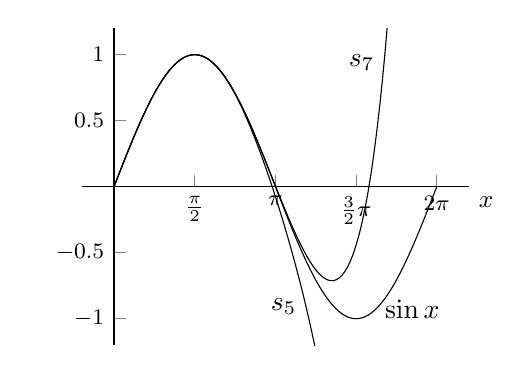
\begin{tikzpicture}
\begin{axis}[small,ymin=-1.2,ymax=1.2,axis lines*=middle,xlabel={$x$},ylabel=\empty,x label style={at={(current axis.right of origin)},anchor=north west},xtick={1.57,3.142,4.71,6.283},xticklabels={$\frac{\pi}{2}$,$\pi$,$\frac{3}{2}\pi$,$2\pi$}]
\addplot[domain=0:2*pi,samples=100]{sin(180/pi*x)}node[pos=0.8,right]{$\sin x$};
\addplot[domain=0:4,samples=100]{x-x^3/6+x^5/120-x^7/5040}node[pos=0.9,left]{$s_5$};
\addplot[domain=0:5.5,samples=100]{x-x^3/6+x^5/120-x^7/5040+x^9/362880}node[pos=0.85,left]{$s_7$};
\end{axis}
\end{tikzpicture}
\caption{سوال \حوالہ{سوال_بیسل_جزوی_تسلسل} کا خط۔\عددی{\sin x} کے علاوہ جزوی مجموعہ \عددی{s_5} اور \عددی{s_7} دکھائے گئے ہیں۔}
\label{شکل_سوال_بیسل_جزوی_تسلسل}
\end{figure}  

\انتہا{سوال}
%======================

\حصہ{لیژانڈر مساوات۔ لیژانڈر کثیر رکنی}\شناخت{حصہ_لیژانڈر_تفاعل}
لیژانڈر تفرقی مساوات\فرہنگ{لیژانڈر!تفرقی مساوات}\حاشیہد{فرانسیسی ریاضی دان اڈریان مری لیژانڈر [1752-1833] نے اعلٰی تفاعل، بیضوی تکمل اور اعدادی نظریہ پر کام کیا۔}\حاشیہب{Legendre's equation}\فرہنگ{Legendre!equation}
\begin{align}\label{مساوات_بیسل_لیژانڈر_الف}
(1-x^2)y''-2xy'+n(n+1)y=0\quad \quad (\text{\RL{\عددی{n} مستقل ہے}})
\end{align} 
طبیعیات کے اہم ترین سادہ تفرقی مساوات میں سے ایک ہے جو متعدد مسائل، بالخصوص کرہ کے سرحدی قیمت مسئلوں، میں سامنے آتی ہے۔ 

مساوات میں \اصطلاح{مقدار معلوم}\فرہنگ{مقدار معلوم} \عددی{n} کی قیمت اصل مسئلے کی نوعیت پر منحصر ہوتی ہے لہٰذا مساوات \حوالہ{مساوات_بیسل_لیژانڈر_الف} درحقیقت سادہ تفرقی مساوات کی \اصطلاح{نسل}\فرہنگ{نسل} کو ظاہر کرتی ہے۔ ہم نے لیژانڈر مساوات، جس میں \عددی{n=1} تھا، کو مثال \حوالہ{مثال_بیسل_کلیہ_توالی_الف} میں حل کیا (جس کو ایک مرتبہ دوبارہ دیکھیں)۔ مساوات \حوالہ{مساوات_بیسل_لیژانڈر_الف} کے کسی بھی حل کو \اصطلاح{لیژانڈر تفاعل}\فرہنگ{لیژانڈر!تفاعل}\حاشیہب{Legendre function}\فرہنگ{Legendre!function} کہتے ہیں۔لیژانڈر تفاعل اور ایسے دیگر اعلٰی تفاعل، جو علم الاحصاء میں نہیں پائے جاتے، کے مطالعہ کو \اصطلاح{نظریہ اعلٰی تفاعل}\فرہنگ{نظریہ!اعلٰی تفاعل}\حاشیہب{special functions theory}\فرہنگ{theory!special functions} کہتے ہیں۔دیگر اعلٰی تفاعل اگلے حصوں میں سامنے آئیں گے۔

مساوات \حوالہ{مساوات_بیسل_لیژانڈر_الف} کو \عددی{1-x^2} سے تقسیم کرتے ہوئے تفرقی مساوات کی معیاری صورت حاصل ہوتی ہے جس کے عددی
 سر \عددی{\tfrac{-2x}{1-x^2}} اور \عددی{\tfrac{n(n+1)}{1-x^2}} نقطہ \عددی{x=0} پر \اصطلاح{تحلیلی} تفاعل ہیں [مثال \حوالہ{مثال_بیسل_تحلیلی_عددی_سر} دیکھیں] لہٰذا لیژانڈر مساوات پر مسئلہ \حوالہ{مسئلہ_بیسل_وجودیت_طاقتی_تسلسل_حل} کا اطلاق ہوتا ہے اور اس کا حل طاقتی تسلسل سے ظاہر کیا جا سکتا ہے۔طاقتی تسلسل
\begin{align}\label{مساوات_بیسل_لیژانڈر_حل_الف}
y=\sum_{m=0}^{\infty}a_mx^m
\end{align}
اور اس کے تفرقات کو مساوات \حوالہ{مساوات_بیسل_لیژانڈر_الف} میں پر کرتے  ہوئے مستقل \عددی{n(n+1)} کو \عددی{k} لکھتے ہوئے
\begin{align*}
(1-x^2)\sum_{m=2}^{\infty}m(m-1)a_mx^{m-2}-2x\sum_{m=1}^{\infty}ma_mx^{m-1}+k\sum_{m=0}^{\infty}a_mx^m=0
\end{align*}
یعنی
\begin{align*}
\sum_{m=2}^{\infty}m(m-1)a_mx^{m-2}-\sum_{m=2}^{\infty}m(m-1)a_mx^m-\sum_{m=1}^{\infty}2ma_mx^{m}+\sum_{m=0}^{\infty}ka_mx^m=0
\end{align*}
حاصل ہوتا ہے۔یہاں آپ مثال \حوالہ{مثال_بیسل_کلیہ_توالی_الف} کی طرح مجموعوں کے چند ابتدائی ارکان لکھ کر آگے بڑھ سکتے ہیں یا پھر درج ذیل طریقہ اختیار کر سکتے ہیں۔ تمام مجموعوں کو  \عددی{x} کی یکساں طاقت کی صورت (\عددی{x^s}) میں لکھنے کی خاطر پہلے مجموعے میں \عددی{s=m-2} یعنی \عددی{m=s+2} پر کرتے ہیں جبکہ بقایا تین مجموعوں میں \عددی{m} کی جگہ \عددی{s} پر کرتے ہیں۔یوں پہلے مجموعے کا پہلا رکن \عددی{m=2} اب \عددی{s=0} ہو گا اور \عددی{a_m} کی جگہ \عددی{a_{s+2}} لکھا جائے گا۔
\begin{align}\label{مساوات_بیسل_لیژانڈر_ب}
\sum_{s=0}^{\infty}(s+2)(s+1)a_{s+2}x^{s}-\sum_{s=2}^{\infty}s(s-1)a_sx^s-\sum_{s=1}^{\infty}2s a_sx^s+\sum_{s=0}^{\infty}ka_s x^s=0
\end{align}
درج بالا مساوات کا دایاں ہاتھ صفر کے برابر ہے لہٰذا مساوات کا بایاں ہاتھ بھی صفر کے برابر ہو گا اور یوں \عددی{x} کے ہر طاقت کے عددی سروں کا مجموعہ صفر کے برابر ہو گا۔یوں \عددی{x^0} کے عددی سر سے شروع کرتے ہوئے باری باری \عددی{x^1}، \عددی{x^2}، \نقطے کے عددی سر صفر کے برابر لکھتے ہیں۔مساوات \حوالہ{مساوات_بیسل_لیژانڈر_ب} کا دوسرا مجموعہ \عددی{x^2} اور تیسرا مجموعہ \عددی{x^1} سے شروع ہوتا ہے لہٰذا ان میں \عددی{x^0} نہیں پایا جاتا ہے۔یوں پہلے اور چوتھے مجموعوں سے \عددی{x^0} کے عددی سر جمع کرتے ہوئے صفر کے برابر پر کرتے ہیں
\begin{align}\label{مساوات_بیسل_لیژانڈر_پ}
2 \cdot 1 a_2+n(n+1)a_0=0
\end{align}
جہاں \عددی{k} کی جگہ واپس \عددی{n(n+1)} لکھا گیا ہے۔ اسی طرح \عددی{x^1} پہلے، تیسرے اور چوتھے مجموعوں میں پایا جاتا ہے جن سے درج ذیل لکھتے ہیں۔
\begin{align}\label{مساوات_بیسل_لیژانڈر_ت}
3\cdot 2 a_3+[-2+n(n+1)]a_1=0
\end{align}
بلند طاقتی اجزاء \عددی{x^2}، \عددی{x^3}، \نقطے تمام مجموعوں میں پائے جاتے ہیں لہٰذا ان کے لئے \عددی{x^s} کے عددی سروں کا مجموعہ لکھتے ہیں۔
\begin{align}\label{مساوات_بیسل_لیژانڈر_ٹ}
(s+2)(s+1)a_{s+2}+[-s(s-1)-2s+n(n+1)]a_s=0
\end{align} 
چکور قوسین \عددی{[\cdots]} کے اندر قوسین کو کھول کر ترتیب دیتے ہوئے درج ذیل لکھا جا سکتا ہے
\begin{align*}
-s(s-1)-2s+n(n+1)&=-s^2+s-2s+n^2+n=n^2-s^2+n-s\\
&=(n-s)(n+s)+n-s\\
&=(n-s)(n+s+1)
\end{align*}
لہٰذا مساوات \حوالہ{مساوات_بیسل_لیژانڈر_ٹ} سے 
\begin{align}\label{مساوات_بیسل_کلیہ_توالی_الف}
a_{s+2}=-\frac{(n-s)(n+s+1)}{(s+2)(s+1)}a_s \quad \quad (s=0,1,\cdots)
\end{align}
حاصل ہوتا ہے جو \اصطلاح{کلیہ توالی}\فرہنگ{کلیہ!توالی}\فرہنگ{توالی کلیہ}\حاشیہب{recurrence relation, recursion formula}\فرہنگ{recursion formula} کہلاتا ہے۔کلیہ توالی کی مدد سے، \عددی{a_0} اور \عددی{a_1} کے علاوہ،  بقایا تمام عددی سر، دو قدم پچھلی عددی سر استعمال کرتے ہوئے دریافت کیے جاتے ہیں۔ یوں \عددی{a_0} اور \عددی{a_1}  اختیاری مستقل ہیں۔ کلیہ توالی کو بار بار استعمال کرتے ہوئے
\begin{gather*}
\begin{aligned}
a_2&=-\frac{n(n+1)}{2!}a_0\\
a_4&=-\frac{(n-2)(n+3)}{4\cdot 3}a_2\\
&=\frac{(n-2)n(n+1)(n+3)}{4!}a_0\\
&\quad\vdots
\end{aligned}\quad\quad
\begin{aligned}
a_3&=-\frac{(n-1)(n+2)}{3!}a_1\\
a_5&=-\frac{(n-3)(n+4)}{5\cdot 4}a_3\\
&=\frac{(n-3)(n-1)(n+2)(n+4)}{5!}a_1\\
&\quad \vdots
\end{aligned}
\end{gather*}
لکھے جا سکتے ہیں جنہیں مساوات \حوالہ{مساوات_بیسل_لیژانڈر_حل_الف} میں پر کرتے ہوئے حل لکھتے ہیں
\begin{align}\label{مساوات_بیسل_حل_لیژانڈر}
y(x)=a_0y_1(x)+a_1y_2(x)
\end{align}
جہاں
\begin{align}\label{مساوات_بیسل_حل_لیژانڈر_الف}
y_1(x)&=1-\frac{n(n+1)}{2!}x^2+\frac{(n-2)n(n+1)(n+3)}{4!}x^4-+\cdots
\end{align}
اور
\begin{align}\label{مساوات_بیسل_حل_لیژانڈر_ب}
y_2(x)&=x-\frac{(n-1)(n+2)}{3!}x^3+\frac{(n-3)(n-1)(n+2)(n+4)}{5!}x^5-+\cdots
\end{align}
ہیں۔یہ تسلسل \عددی{\abs{x}<1} کے لئے مرکوز ہیں۔بعض اوقات تسلسل کا کوئی عددی سر صفر کے برابر حاصل ہوتا ہے اور یوں کلیہ توالی کے تحت اگلے تمام عددی سر بھی صفر ہوں گے اور یوں تسلسل محدود ارکان پر مشتمل ہوتا ہے۔چونکہ مساوات \حوالہ{مساوات_بیسل_حل_لیژانڈر_الف} میں \عددی{x} کے جفت طاقت پائے جاتے ہیں جبکہ مساوات \حوالہ{مساوات_بیسل_حل_لیژانڈر_ب} میں \عددی{x} کے طاق طاقت پائے جاتے ہیں لہٰذا \عددی{\tfrac{y_1}{y_2}} مستقل مقدار نہیں ہو سکتا ہے اور یوں \عددی{y_1} اور \عددی{y_2} آپس میں خطی تعلق نہیں رکھتے لہٰذا یہ خطی طور غیر تابع حل ہیں۔یوں مساوات \حوالہ{مساوات_بیسل_حل_لیژانڈر} کھلے وقفہ \عددی{-1<x<1} پر عمومی حل ہے۔

دھیان رہے کہ \عددی{x=\mp 1} پر \عددی{1-x^2=0} ہو گا لہٰذا سادہ تفرقی مساوات کی معیاری صورت میں عددی سر غیر تحلیلی ہوں گے۔یوں حیرانی کی بات نہیں ہے کہ تسلسل \حوالہ{مساوات_بیسل_حل_لیژانڈر_الف} اور تسلسل \حوالہ{مساوات_بیسل_حل_لیژانڈر_الف} کا ارتکازی وقفہ وسیع نہیں ہے ماسوائے اس صورت میں جب  اجزاء کی تعداد محدود ہونے کی بنا  تسلسل کثیر رکنی کی صورت اختیار کرے۔
%=====================

\جزوحصہء{کثیر رکنی حل۔ لیژانڈر کثیر رکنی \عددی{P_n(x)}}
طاقتی تسلسل کے تخفیف سے کثیر رکنی حاصل ہوتی ہے جس کا حل، ارتکازی شرط کے قید سے آزاد،  تمام \عددی{x} کے لئے پایا جاتا ہے۔ایسے اعلٰی تفاعل جو سادہ تفرقی مساوات کے حل ہوتے ہیں میں یہ صورت عموماً پائی جاتی ہے جن سے مختلف نسل کے اہم کثیر رکنی حاصل ہوتے ہیں۔لیژانڈر مساوات میں \عددی{n} کی قیمت غیر منفی عدد صحیح ہونے کی صورت میں \عددی{s=n} پر مساوات \حوالہ{مساوات_بیسل_کلیہ_توالی_الف} صفر کے برابر ہوتا ہے لہٰذا \عددی{a_{n+2}=0} ہو گا اور یوں \عددی{a_{n+4}=0}، \عددی{a_{n+6}=0}، \نقطے ہوں گے۔جفت \عددی{n} کی صورت میں \عددی{y_1} کثیر رکنی ہو گا جبکہ طاق \عددی{n} کی صورت میں \عددی{y_2} کثیر رکنی ہو گا۔ان کثیر رکنی کو مستقل مقدار سے ضرب دیتے ہوئے \اصطلاح{لیژانڈر کثیر رکنی}\فرہنگ{لیژانڈر!کثیر رکنی}\حاشیہب{Legendre polynomial}\فرہنگ{Legendre!polynomial} حاصل ہوتی ہیں جنہیں \عددی{P_n(x)} سے ظاہر کیا جاتا ہے۔روایتی طور پر اس مستقل مقدار کو درج ذیل طریقے سے چننا جاتا ہے۔

تسلسل میں \عددی{x^n} کے عددی سر \عددی{a_n} کو
\begin{align}\label{مساوات_بیسل_روایتی_سر_الف}
a_n=\frac{(2n)!}{2^n(n!)^2}=\frac{1\cdot 3 \cdot 5\cdots (2n-1) }{n!} \quad \quad \text{\RL{\عددی{n} مثبت عدد ہے}}
\end{align}
چننا [مثال \حوالہ{مثال_بیسل_لیژانڈر_عددی_سر} دیکھیں] جاتا ہے (جبکہ \عددی{n=0} کی صورت میں \عددی{a_n=1} چننا جاتا ہے)۔ مساوات \حوالہ{مساوات_بیسل_کلیہ_توالی_الف} کو ترتیب دیتے ہوئے درج ذیل لکھا جا سکتا ہے جسے استعمال کرتے ہوئے دیگر عددی سر حاصل کیے جاتے ہیں۔
\begin{align}\label{مساوات_بیسل_روایتی_سر_ب}
a_s=-\frac{(s+2)(s+1)}{(n-s)(n+s+1)}a_{s+2}\quad \quad (s \le n-2)
\end{align}
کثیر رکنی میں \عددی{x} کی بلند تر طاقت  کے عددی سر \عددی{a_n} کو مساوات \حوالہ{مساوات_بیسل_روایتی_سر_الف} کے تحت چننے سے \عددی{x=1} پر تمام \عددی{P_n} کی قیمت اکائی \عددی{[P_n(1)=1]} حاصل ہوتی ہے [شکل \حوالہ{شکل_لیژانڈر_کثیر_رکنی} دیکھیں]۔یہی \عددی{a_n} یوں چننے کی وجہ ہے۔مساوات \حوالہ{مساوات_بیسل_روایتی_سر_ب} میں \عددی{s+2=n} یعنی \عددی{s=n-2} پر کرتے ہوئے  مساوات \حوالہ{مساوات_بیسل_روایتی_سر_الف} سے \عددی{a_n} پر کرتے ہیں۔ 
\begin{align*}
a_{n-2}=-\frac{n(n-1)}{2(2n-1)}a_n=-\frac{n(n-1)}{2(2n-1)} \frac{(2n)!}{2^n(n!)^2}
\end{align*}
شمار کنندہ میں \عددی{(2n)!=2n(2n-1)(2n-2)!} اور نسب نما میں \عددی{(n!)^2} کو \عددی{n! n!} لکھ کر اس  میں \عددی{n!=n(n-1)!}  اور \عددی{n!=n(n-1)(n-2)!} پر کرتے ہوئے
\begin{align*}
a_{n-2}&=-\frac{n(n-1)}{2(2n-1)} \frac{2n(2n-1)(2n-2)!}{2^n n(n-1)! n(n-1)(n-2)!}\\
&=-\frac{(2n-2)!}{2^n(n-1)!(n-2)!}
\end{align*}
ملتا ہے جہاں \عددی{n(n-1)2n(2n-1)} کٹ جاتے ہیں۔اسی طرح
\begin{align*}
a_{n-4}&=-\frac{(n-2)(n-3)}{4(2n-3)}a_{n-2}\\
&=\frac{(2n-4)!}{2^n2!(n-2)!(n-4)!}
\end{align*}
اور دیگر عددی سر حاصل کیے جا سکتے ہیں۔یوں درج ذیل عمومی کلیہ لکھا جا سکتا ہے۔
\begin{align}
a_{n-2m}=(-1)^m\frac{(2n-2m)!}{2^nm!(n-m)!(n-2m)!}\quad \quad (n-2m \ge 0)
\end{align}
ان عددی سر کو استعمال کرتے ہوئے لیژانڈر تفرقی مساوات \حوالہ{مساوات_بیسل_لیژانڈر_الف} کا کثیر رکنی حل
\begin{gather}
\begin{aligned}\label{مساوات_بیسل_لیژانڈر_عمومی_الف}
P_n(x)&=\sum_{m=0}^{M} (-1)^m\frac{(2n-2m)!}{2^nm!(n-m)!(n-2m)!} x^{n-2m}\\
&=\frac{(2n)!}{2^n(n!)^2}x^n-\frac{(2n-2)!}{2^n 1!(n-1)!(n-2)!}x^{n-2}+-\cdots
\end{aligned}
\end{gather}
 حاصل ہوتا ہے۔اب \عددی{\tfrac{n}{2}} یا \عددی{\tfrac{n-1}{2}} عدد صحیح ہو گا اور \عددی{M} اس عدد صحیح کے برابر ہو گا [مثال \حوالہ{مثال_بیسل_ثبوت_ایم} دیکھیں]۔درج بالا  \عددی{n} درجی \اصطلاح{لیژانڈر کثیر رکنی}\فرہنگ{لیژانڈر!کثیر رکنی}\حاشیہب{Legendre polynomial}\فرہنگ{Legendre!polynomial} کہلاتا ہے اور اس کو \عددی{P_n(x)} سے ظاہر کیا جاتا ہے۔ چند پہلے لیژانڈر کثیر رکنی جنہیں شکل \حوالہ{شکل_لیژانڈر_کثیر_رکنی} میں دکھایا گیا ہے درج ذیل ہیں۔
\begin{gather}
\begin{aligned}\label{مساوات_بیسل_لیژانڈر_عمومی_ب}
P_0(x)&=1\\
P_2(x)&=\frac{1}{2}(3x^2-1)\\
P_4(x)&=\frac{1}{8}(35x^4-30x^2+3)
\end{aligned}\quad \quad
\begin{aligned}
P_1(x)&=x\\
P_3(x)&=\frac{1}{2}(5x^3-3x)\\
P_5(x)&=\frac{1}{8}(63x^5-70x^3+15x)
\end{aligned}
\end{gather}
%
\begin{figure}
\centering
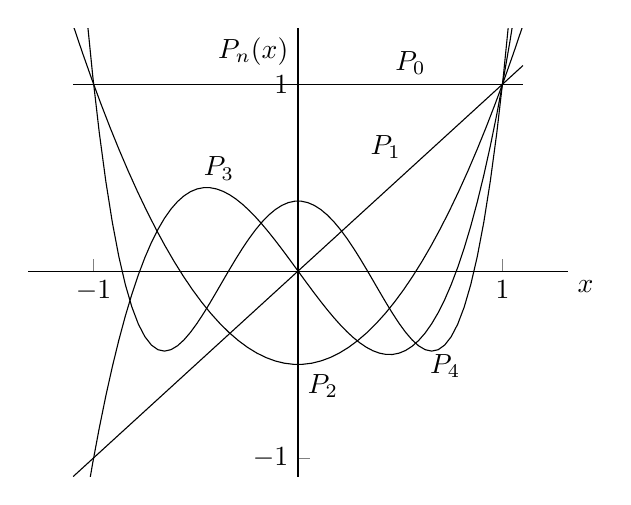
\begin{tikzpicture}
\begin{axis}[axis lines*=middle,ymin=-1.1,ymax=1.3,xlabel={$x$},ylabel={$P_n(x)$},xlabel style={at={(current axis.right of origin)},anchor=north west}, ylabel style={at={(current axis.above origin)},anchor=north east},ylabel style={rotate=-90},ytick={-1,1},yticklabels={$-1$,$1$},xtick={-1,1},xticklabels={$-1$,$1$}]
\pgfmathsetmacro{\lmt}{1.1}
%
\addplot[domain=-\lmt:\lmt]{1}node[pos=0.75,above]{$P_0$};
\addplot[domain=-\lmt:\lmt,samples=50]{1/2*(3*x^2-1)}node[pos=0.5,below right]{$P_2$};
\addplot[domain=-\lmt:\lmt,samples=70]{1/8*(35*x^4-30*x^2+3)}node[pos=0.65,below]{$P_4$};
\addplot[domain=-\lmt:\lmt]{x}node[pos=0.75,above left]{$P_1$};
\addplot[domain=-\lmt:\lmt,samples=70]{1/2*(5*x^3-3*x)}node[pos=0.4,above]{$P_3$};
\end{axis}
\end{tikzpicture}
\caption{لیژانڈر کثیر رکنی۔}
\label{شکل_لیژانڈر_کثیر_رکنی}
\end{figure}

لیژانڈر کثیر رکنی \عددی{P_n(x)} وقفہ \عددی{-1 \le x \le 1} پر آپس میں \اصطلاح{قائمہ الزاویہ}\فرہنگ{قائمہ الزاویہ}\حاشیہب{orthogonal}\فرہنگ{orthogonal} ہیں۔یہ خصوصیت \اصطلاح{فوریئر لیژانڈر} تسلسل کے لئے ضروری ہے جن پر اسی باب میں غور کیا جائے گا۔
%==============
\ابتدا{مثال}\شناخت{مثال_بیسل_تحلیلی_عددی_سر}
لیژانڈر مساوات \حوالہ{مساوات_بیسل_لیژانڈر_الف} \عددی{1-x^2} سے تقسیم کرتے ہوئے معیاری صورت میں لکھتے ہوئے ثابت کریں کی اس کے عددی سر \عددی{x=0} پر  تحلیلی ہیں۔

حل:لیژانڈر مساوات کو \عددی{1-x^2} سے تقسیم کرتے ہوئے \عددی{y''-\tfrac{2x}{1-x^2}y'+\tfrac{n(n+1)}{1-x^2}=0} حاصل ہوتا ہے جس کے عددی سر \عددی{\tfrac{-2x}{1-x^2}} اور \عددی{\tfrac{n(n+1)}{1-x^2}} ہیں جن کی مکلارن تسلسل درج ذیل ہیں۔
\begin{align*}
\frac{n(n+1)}{1-x^2}&=n(n+1)(1+x^2+x^4+\cdots)\\
\frac{-2x}{1-x^2}&=-2(x+x^3+x^5+\cdots)
\end{align*}
پہلی تسلسل کا \عددی{\tfrac{a_{m+1}}{a_m}=1} ہیں لہٰذا اس کا رداس ارتکاز \عددی{R=1} ہے۔دوسری تسلسل کا بھی \عددی{\tfrac{a_{m+1}}{a_m}=1} اور \عددی{R=1} ہیں۔یوں دونوں تسلسل تحلیلی ہیں۔
\انتہا{مثال}
%===============
\ابتدا{مثال}\شناخت{مثال_بیسل_لیژانڈر_عددی_سر}
درج ذیل مساوات کے بائیں ہاتھ سے اس کا دایاں ہاتھ حاصل کریں۔
\begin{align*}
\frac{(2n)!}{2^n(n!)^2}=\frac{1\cdot 3\cdot 5\cdots (2n-1)}{n!}
\end{align*}

حل:پہلے  \عددی{n=3} کے لئے حل کرتے ہیں۔یوں درج ذیل لکھا جا سکتا ہے جہاں شمار کنندہ میں طاق اعداد (جو طاق مقامات پر پائے جاتے ہیں) کو ایک طرف اور جفت اعداد (جو جفت مقامات پر پائے جاتے ہیں) کو دوسری طرف منتقل کرتے ہوئے ہر جفت عدد سے \عددی{2} کا ہندسہ نکالا گیا ہے۔ 
\begin{align*}
\frac{(2\cdot 3)!}{2^3(3!)^2}=\frac{6\cdot 5\cdot 4\cdot 3\cdot 2\cdot 1}{2^3(3\cdot 2\cdot 1)^2}=\frac{6\cdot 4\cdot 2\cdot 5\cdot 3\cdot 1}{2^3(3!)^2}=\frac{2^3(3\cdot 2\cdot 1)\cdot 5\cdot 3\cdot 1}{2^3(3!)^2}=\frac{5\cdot 3\cdot 1}{3!}
\end{align*}
شمار کنندہ میں اعداد کو ترتیب دیتے ہوئے اور اس میں سب سے بڑے عدد \عددی{5} کو \عددی{2\cdot 3-1} لکھتے ہوئے  \عددی{\tfrac{1\cdot 3\cdot (2\cdot 3-1)}{3!}} لکھا جا سکتا ہے۔ آئیں یہی سب کچھ عمومی عددی صحیح \عددی{n} کے لئے ثابت کریں۔
\begin{align*}
\frac{(2n)!}{2^n(n!)^2}&=\frac{2n(2n-1)(2n-2)(2n-3)(2n-4)(2n-5)\cdots 8\cdot 7\cdot 6\cdot 5 \cdot 4\cdot 3\cdot 2\cdot 1 }{2^n(n!)^2}\\
&=\frac{2n(2n-2)(2n-4)\cdots 8\cdot 6\cdot 4\cdot 2\cdot (2n-1)(2n-3)(2n-5)\cdots 7\cdot 5\cdot 3\cdot 1}{2^n(n!)^2}\\
&=\frac{2^n n(n-1)(n-2)\cdots 4\cdot 3\cdot 2\cdot 1\cdot (2n-1)(2n-3)(2n-5)\cdots 7\cdot 5\cdot 3\cdot 1}{2^n(n!)^2}\\
&=\frac{(2n-1)(2n-3)(2n-5)\cdots 7\cdot 5\cdot 3\cdot 1}{n!}\\
&=\frac{1\cdot 3\cdot 5\cdots (2n-1)}{n!}
\end{align*}

\انتہا{مثال}
%==========================
\ابتدا{مثال}\شناخت{مثال_بیسل_ثبوت_ایم}
لیژانڈر کثیر رکنی مجموعہ [مساوات \حوالہ{مساوات_بیسل_لیژانڈر_عمومی_الف}] کی بالائی حد \عددی{M} ہے۔\عددی{M} کی قیمت دریافت کریں۔

حل:مساوات \حوالہ{مساوات_بیسل_کلیہ_توالی_الف} لیژانڈر کثیر رکنی کے عددی سر دیتی ہے جس کے تحت \عددی{s=n} پر عددی سر صفر \عددی{(a_{n+2}=0)} کے برابر ہو گا اور یوں بقایا عددی سر \عددی{a_{n+4}}، \عددی{a_{n+6}}، \نقطے بھی صفر کے برابر ہوں گے۔یوں کثیر رکنی میں \عددی{x} کی زیادہ سے زیادہ طاقت \عددی{n} ہو گی۔اس طرح \عددی{n=5} کی صورت میں \عددی{a_5x^5}، \عددی{a_3x^3} اور \عددی{a_1x^1} پایا جائے گا جبکہ \عددی{n=8} کی صورت میں \عددی{a_8x^8}، \عددی{a_6x^6}، \عددی{a_4x^4}، \عددی{a_2x^2} اور \عددی{a_0} پائے جائیں گے۔ آپ نے دیکھا کہ طاق \عددی{n} کی صورت میں کثیر رکنی میں کل \عددی{\tfrac{n-1}{2}} پائے گئے جبکہ جفت \عددی{n} کی صورت میں ارکان کی تعداد \عددی{\tfrac{n}{2}} تھی۔یوں طاق \عددی{n} کی صورت میں \عددی{M=\tfrac{n-1}{2}}  اور جفت \عددی{n} کی صورت میں \عددی{M=\tfrac{n}{2}} ہو گا جہاں \عددی{M} عدد صحیح ہے۔ 
\انتہا{مثال}
%========================

\ابتدا{مثال}\quad (\اصطلاح{کلیہ روڈریگیس})\\
تفاعل \عددی{(x^2-1)^n} کو \اصطلاح{الکراجی کے مسئلہ ثنائی}\فرہنگ{الکراجی کا مسئلہ ثنائی}\فرہنگ{مسئلہ ثنائی، الکراجی}\حاشیہد{\تحریر{binomial theorem}\,\, ابو بکر ابن محمد ابن الحسین الکراجی [953-1029] ایرانی ریاضی دان۔} سے پھیلا کر اس کا \عددی{n} درجی تفرق لیں۔حاصل جواب کا مساوات \حوالہ{مساوات_بیسل_لیژانڈر_عمومی_الف} کے ساتھ موازنہ کرتے ہوئے درج ذیل کلیہ حاصل کریں جس کو \اصطلاح{کلیہ روڈریگیس}\فرہنگ{کلیہ!روڈریگیس}\فرہنگ{روڈریگیس کلیہ}\حاشیہد{\تحریر{Rodrigues' formula}  \,\, فرانسیسی ریاضی دان بنجامن اولانڈے روڈریگیس [1794-1851]}\فرہنگ{Rodrigues' formula} کہتے ہیں۔
\begin{align}\label{مساوات_بیسل_روڈریگیس_مساوات}
P_n(x)=\frac{1}{2^n n!}\frac{\dif^{\,n}}{\dif x^n}[(x^2-1)^n]
\end{align}

حل:\عددی{(x^2-1)^n} کو مسئلہ الکراجی سے پھیلاتے ہوئے \عددی{n+1} ارکان ملتے ہیں۔
\begin{multline}\label{مساوات_سوال_بیسل_الکرازی_الف}
y=(x^2-1)^n=(x^2)^n+\frac{n}{1!}(x^2)^{n-1}(-1)^1+\frac{n(n-1)}{2!}(x^2)^{n-2}(-1)^2+\cdots   \\
+\frac{n(n-1)}{2!}(x^2)^2(-1)^{n-2}+\frac{n}{1!}(x^2)(-1)^{n-1}+(-1)^n
\end{multline}
اس مساوات کا آخری رکن مستقل مقدار \عددی{(-1)^n} ہے جبکہ اس رکن سے ایک پہلے  رکن میں \عددی{x^2} پایا جاتا ہے۔یوں \عددی{y'} لینے سے آخری رکن صفر ہو جائے گا لہٰذا \عددی{y'} میں \عددی{n} ارکان رہ جائیں گے۔\عددی{y'} کے آخری رکن میں \عددی{x^1} پایا جائے گا۔\عددی{y''} لینے سے یہ رکن مستقل مقدار ہو جائے گا جبکہ ارکان کی تعداد میں مزید کمی رو نما نہیں ہو گی۔اسی طرح \عددی{y'''} لینے سے ایک اور رکن کم ہو جائے گا اور \عددی{n-1} ارکان رہ جائیں گے۔\عددی{y''''} لینے سے ارکان کی تعداد میں کمی پیدا نہیں ہو گی۔یوں ہر دو مرتبہ تفرق لینے سے تعداد اکائی کمی پیدا ہو گی۔ آپ دیکھ سکتے ہیں کہ \عددی{n} درجی تفرق \عددی{y^{(n)}} لینے کے بعد ارکان کی تعداد  \عددی{\tfrac{n}{2}} یا \عددی{\tfrac{n-1}{2}} ہو گی جس کو ہم \عددی{M} سے ظاہر کرتے ہیں اور جو صحیح عدد ہو گا۔
 
 مساوات \حوالہ{مساوات_سوال_بیسل_الکرازی_الف} کو مجموعے کی صورت میں لکھتے ہیں جس میں \عددی{m=0} تا \عددی{m=n} ارکان  یعنی \عددی{n+1} ارکان ہیں۔
\begin{align}\label{مساوات_سوال_بیسل_الکرازی_ب}
y=\sum_{m=0}^{n} \frac{n!(x^2)^{n-m}(-1)^m}{(n-m)!m!}=\sum_{m=0}^{n} \frac{n!(-1)^m}{(n-m)!m!}x^{2n-2m}
\end{align}

اب \عددی{z=x^{2n-2m}} پر نظر رکھیں۔اس کے تفرق لیتے ہیں۔
\begin{align*}
z'&=(2n-2m)x^{2n-2m-1}=\frac{(2n-2m)!}{(2n-2m-1)!}x^{2n-2m-1}\\
z''&=(2n-2m)(2n-2m-1)x^{2n-2m-2}=\frac{(2n-2m)!}{(2n-2m-2)!}x^{2n-2m-2}\\
z'''&=(2n-2m)(2n-2m-1)(2n-2m-2)x^{2n-2m-3}=\frac{(2n-2m)!}{(2n-2m-3)!}x^{2n-2m-3}\\
&\vdots\\
z^{(k)}&=\frac{(2n-2m)!}{(2n-2m-k)!}x^{2n-2m-k}\\
z^{(n)}&=\frac{(2n-2m)!}{(2n-2m-n)!}x^{2n-2m-n}=\frac{(2n-2m)!}{(n-2m)!}x^{n-2m}
\end{align*}
ان نتائج  کو استعمال کرتے ہوئے مساوات \حوالہ{مساوات_سوال_بیسل_الکرازی_ب} کا \عددی{n} درجی تفرق لکھتے ہیں
 \begin{align*}
y^{(n)}=\frac{\dif^{\,n}}{\dif x^n}[(x^2-1)^n]=\sum_{m=0}^{M} \frac{n!(-1)^m}{(n-m)!m!}\frac{(2n-2m)!}{(n-2m)!}x^{n-2m}
\end{align*}
جس کا مساوات \حوالہ{مساوات_بیسل_لیژانڈر_عمومی_الف} کے ساتھ موازنہ کرتے ہوئے درج ذیل لکھا جا سکتا ہے۔
\begin{align*}
P_n(x)=\frac{1}{2^n n!}\frac{\dif^{\,n}}{\dif x^n}[(x^2-1)^n]
\end{align*}
\انتہا{مثال}
%=======================
\ابتدا{مثال}
روڈریگیس مساوات \حوالہ{مساوات_بیسل_روڈریگیس_مساوات} استعمال کرتے ہوئے \عددی{n} مرتبہ تکمل بالحصص لیتے ہوئے درج ذیل ثابت کریں۔
\begin{align*}
\int_{-1}^{1} P_n^2(x) \dif x=\frac{2}{2n+1}\quad \quad (n=0,1,\cdots)
\end{align*}

حل :فرض کریں کہ \عددی{y=(x-1)^3} ہے۔یوں \عددی{y'=3(x-1)^2}، \عددی{y''=3\cdot 2(x-1)}، \عددی{y'''=3\cdot 2\cdot 1 } اور \عددی{y^{(4)}=0} ہوں گے جن  سے \عددی{y(1)=0}، \عددی{y'(1)=0}، \عددی{y''(1)=0}، \عددی{y'''(1)=3!} اور \عددی{y(1)^{(4)}=0} حاصل ہوتے ہیں۔اس سے ہم اخذ کرتے ہیں کہ \عددی{y_1=(x-1)^n} کی صورت میں
\begin{align}\label{مساوات_بیسل_سوال_عمومی_الف}
y_1=(x-1)^n,\quad y_1^{(m)}=\frac{n!}{(n-m)!}(x-1)^{n-m},\quad y_1^{(m)}(1)=n! \,\delta_{n,m}
\end{align}
اور \عددی{y_2=(x+1)^n} کی صورت میں
\begin{align}\label{مساوات_بیسل_سوال_عمومی_ب}
y_2=(x-1)^n,\quad y_2^{(m)}=\frac{n!}{(n-m)!}(x+1)^{n-m},\quad y_2^{(m)}(-1)=n! \,\delta_{n,m}
\end{align}
ہو گا جہاں \عددی{\delta_{n,m}} کی تعریف درج ذیل ہے (یعنی \عددی{m=n} کی صورت میں \عددی{\delta=1} جبکہ \عددی{m \ne n} کی صورت میں \عددی{\delta =0} ہے)۔ 
\begin{align}\label{مساوات_بیسل_کرونیکر_الف}
\delta_{n,m}=
\begin{cases}
1& n=m\\
0&n \ne m
\end{cases}
\end{align}
مساوات \حوالہ{مساوات_بیسل_سوال_عمومی_الف} کہتی ہے کہ \عددی{y_1=(x-1)^n} کے تمام تفرقات کی قیمت \عددی{x=1} پر صفر ہو گی ماسوائے \عددی{n} درجی تفرق، جس کی قیمت \عددی{n!} ہو گی۔  مساوات \حوالہ{مساوات_بیسل_سوال_عمومی_ب} یہی کچھ \عددی{y_2=(x+1)^n} کے بارے میں \عددی{x=-1} پر کہتی ہے۔

اب اگر \عددی{X=(x^2-1)^n=(x-1)^n(x+1)^n=y_1y_2} ہو تب \اصطلاح{کلیہ لیبنٹز}\فرہنگ{کلیہ لیبنٹز}\فرہنگ{لیبنٹز کلیہ}\حاشیہب{Leibnitz formula}\فرہنگ{Leibnitz formula} سے درج ذیل لکھا جاتا ہے۔
\begin{align*}
\frac{\dif^{\, m}X}{\dif x^m}=\sum_{s=0}^{m}\binom{m}{s}\overbrace{\frac{\dif^{\,m-s}y_1}{\dif x^{m-s}}}^{M}\cdot \overbrace{\frac{\dif^{\,s}y_2}{\dif x^s}}^{N}
\end{align*}
اگر \عددی{m \ne n} ہو، اور بالخصوص اگر \عددی{m<n} ہو، تب مساوات \حوالہ{مساوات_بیسل_سوال_عمومی_الف} کہتی ہے کہ  \عددی{M(x=1)=0} ہو گا جبکہ مساوات \حوالہ{مساوات_بیسل_سوال_عمومی_ب} کہتی ہے کہ تب \عددی{N(x=-1)=0} ہو گا۔ان نتائج کی بنا درج ذیل حاصل ہوتا ہے۔
\begin{align}\label{مساوات_بیسل_سوال_عمومی_پ}
\frac{\dif^{\, m}X}{\dif x^m}=0
\end{align}
مساوات \حوالہ{مساوات_بیسل_روڈریگیس_مساوات} کو استعمال کرتے ہوئے
$P_n=\frac{1}{2^n n!} \frac{\dif^{\,n} [(x^2-1)^n]}{\dif x^n}=\frac{1}{2^n n!} \frac{\dif^{\,n} X}{\dif x^n}$
لکھا جا سکتا ہے لہٰذا
\begin{align*}
\int_{-1}^{1} P_n^2  \dif x&=\frac{1}{2^{2n}(n!)^2}\int_{-1}^{1}\frac{\dif^{\,n} X}{\dif x^n} \cdot \frac{\dif^{\,n}X}{\dif x^n} \dif x\\
&=\frac{1}{2^{2n}(n!)^2}\left[\frac{\dif^{\,n} X}{\dif x^n} \cdot \left. \frac{\dif^{\,n-1}X}{\dif x^{n-1}}\right|_{-1}^{1}-\int_{-1}^{1}\frac{\dif^{\,n+1} X}{\dif x^{n+1}} \cdot \frac{\dif^{\,n-1}X}{\dif x^{n-1}} \dif x\right]
\end{align*}
ہو گا جہاں تکمل بالحصص استعمال کیا گیا ہے۔مساوات \حوالہ{مساوات_بیسل_سوال_عمومی_پ} کے تحت
 \عددی{\left.\frac{\dif^{\, n-1}X}{\dif x^{n-1}}\right|_1=\left.\frac{\dif^{\, n-1}X}{\dif x^{n-1}}\right|_{-1}=0} ہے لہٰذا آخری قدم پر تکمل کے باہر تمام حصہ صفر کے برابر ہے اور یوں  درج ذیل حاصل ہوتا ہے
\begin{align*}
\int_{-1}^{1} P_n^2  \dif x&=\frac{-1}{2^{2n}(n!)^2}\int_{-1}^{1}\frac{\dif^{\,n+1} X}{\dif x^{n+1}} \cdot \frac{\dif^{\,n-1}X}{\dif x^{n-1}}\dif x\\
&=\frac{-1}{2^{2n}(n!)^2}\left[\frac{\dif^{\,n+1} X}{\dif x^{n+1}} \cdot \left. \frac{\dif^{\,n-2}X}{\dif x^{n-2}}\right|_{-1}^{1}-\int_{-1}^{1}\frac{\dif^{\,n+2} X}{\dif x^{n+2}} \cdot \frac{\dif^{\,n-2}X}{\dif x^{n-2}}\dif x \right]
\end{align*}
جہاں دوبارہ تکمل بالحصص لیا گیا ہے۔پہلی کی طرح اب بھی تکمل کا باہر والا حصہ صفر کے برابر ہے۔ اسی طرح بار بار تکمل بالحصص لیتے ہوئے ہر بار بیرونی حصہ صفر کے برابر حاصل ہوتا ہے۔یوں \عددی{s} مرتبہ تکمل لیتے اور بیرونی حصے کو صفر پر کرتے ہوئے درج ذیل ملتا ہے۔
 \begin{align*}
\int_{-1}^{1} P_n^2  \dif x&=\frac{(-1)^s}{2^{2n}(n!)^2}\int_{-1}^{1}\frac{\dif^{\,n+s} X}{\dif x^{n+s}} \cdot \frac{\dif^{\,n-s}X}{\dif x^{n-s}}\dif x
\end{align*}
آخر کار \عددی{s=n} ہو گا اور یوں درج ذیل حاصل ہو گا جہاں \عددی{\tfrac{\dif^{\,0} X}{\dif x^0}=X} لکھا گیا ہے۔
 \begin{align*}
\int_{-1}^{1} P_n^2  \dif x&=\frac{(-1)^n}{2^{2n}(n!)^2}\int_{-1}^{1}\frac{\dif^{\,n+n} X}{\dif x^{n+n}} \cdot \frac{\dif^{\,n-n}X}{\dif x^{n-n}} \dif x=\frac{(-1)^n}{2^{2n}(n!)^2}\int_{-1}^{1}\frac{\dif^{\,2n} X}{\dif x^{2n}} \cdot X \dif x
\end{align*}
 \عددی{X=(x^2-1)^n} کا الکراجی ثنائی تسلسل مساوات \حوالہ{مساوات_سوال_بیسل_الکرازی_الف} دیتی ہے جس کا\عددی{2n} درجی تفرق لینے سے، پہلے رکن کے علاوہ، تمام ارکان صفر کے برابر ہو جاتے ہیں۔یوں اس کا \عددی{2n} درجی تفرق \عددی{\frac{\dif^{\, 2n}X}{\dif x^{2n}}=(2n)!}  ہو گا جس سے درج بالا تکمل یوں
 \begin{align}\label{مساوات_بیسل_سوال_عمومی_ت}
\int_{-1}^{1} P_n^2  \dif x&=\frac{(-1)^n (2n)!}{2^{2n}(n!)^2}\int_{-1}^{1} X \dif x
\end{align}
لکھا جاتا ہے۔آئیں \عددی{\int X\dif x} کو تکمل بالحصص کے ذریعہ حاصل کریں۔
\begin{align*}
\int_{-1}^{1}X\dif x&=\int_{-1}^{1} (x-1)^n(x+1)^n\dif x\\
&=\left.(x-1)^n\frac{(x+1)^{n+1}}{n+1} \right|_{-1}^{1}-\int_{-1}^{1} n(x-1)^{n-1}\frac{(x+1)^{n+1}}{n+1}\dif x
\end{align*}
تکمل کے باہر حصہ صفر کے برابر ہے۔اسی طرح بار بار تکمل بالحصص لیتے ہوئے ہر مرتبہ تکمل کے باہر حصہ صفر کے برابر حاصل ہوتا ہے۔\عددی{s} مرتبہ تکمل بالحصص لیتے ہوئے اور تکمل کے باہر حصے کو صفر کے برابر پر کرتے ہوئے  درج ذیل ملتا ہے۔
\begin{align*}
\int_{-1}^{1}X\dif x&=(-1)^s\int_{-1}^{1} [n(n-2)\cdots (n-s+1)](x-1)^{n-s}\frac{(x+1)^{n+s}}{(n+1)(n+2)\cdots (n+s)}\dif x\\
&=(-1)^s\int_{-1}^{1} \frac{n! (x-1)^{n-s}}{(n-s)!} \frac{n!(x+1)^{n+s}}{(n+s)!}
\end{align*}
آخر کار \عددی{s=n} ہو گا جس پر درج ذیل لکھا جائے گا
\begin{align*}
\int_{-1}^{1}X\dif x&=(-1)^n\int_{-1}^{1} \frac{n! (x-1)^{n-n}}{(n-n)!} \frac{n!(x+1)^{n+n}}{(n+n)!}\\
&=\frac{(-1)^n(n!)^2}{(2n)!}\int_{-1}^{1} (x+1)^{2n}\\
&=\left. \frac{(-1)^n(n!)^2}{(2n)!}\frac{(x+1)^{2n+1}}{2n+1}\right|_{-1}^{1}\\
&=\frac{(-1)^n(n!)^2}{(2n)!}\frac{2^{2n+1}}{2n+1}
\end{align*}
جہاں \عددی{0!=1}  (مساوات \حوالہ{مساوات_بیسل_گیما_پ}) پر کیا گیا ہے۔درج بالا نتیجے کو مساوات \حوالہ{مساوات_بیسل_سوال_عمومی_ت} میں پر کرتے ہیں
 \begin{align}\label{مساوات_طاقتی_لیژانڈر_معیار}
\int_{-1}^{1} P_n^2  \dif x&=\frac{(-1)^n (2n)!}{2^{2n}(n!)^2}\frac{(-1)^n(n!)^2}{(2n)!}\frac{2^{2n+1}}{2n+1}=\frac{2}{2n+1}
\end{align}
جہاں منفی ایک کا جفت طاقت اکائی کے برابر \عددی{[(-1)^{2n}=1]} ہے۔
\انتہا{مثال}
%=========================
\ابتدا{مثال}
درج ذیل ثابت کریں جہاں \عددی{n \ne m} ہے۔
\begin{align}
\int_{-1}^{1}P_nP_m \dif x=0\quad \quad (n \ne m)
\end{align}

حل: فرض کریں کہ \عددی{X=(x^2-1)^n} اور \عددی{Y=(x^2-1)^m} ہیں۔ یوں مساوات \حوالہ{مساوات_بیسل_روڈریگیس_مساوات} کے تحت
 \عددی{P_n=\tfrac{1}{2^n n!}\tfrac{\dif^{\, n} X}{\dif x^n}} اور  \عددی{P_m=\tfrac{1}{2^m m!}\tfrac{\dif^{\, m} Y}{\dif x^m}}  ہوں گے لہٰذا
\begin{align*}
\int_{-1}^{1}P_n P_m \dif x=\frac{1}{2^{n+m}n!m!}\int_{-1}^{1} \frac{\dif^{\,n}X}{\dif x^n}\cdot \frac{\dif^{\,m}Y}{\dif x^m}\dif x
\end{align*}
ہو گا۔چونکہ \عددی{n} اور \عددی{m} برابر نہیں ہیں لہٰذا ان میں ایک کی قیمت دوسرے سے کم ہو گی۔ہم فرض کرتے ہیں کہ \عددی{n<m} ہے۔گزشتہ مثال کی طرح، درج بالا کو بار بار تکمل بالحصص سے حل کرتے ہوئے، ہر بار تکمل کے باہر حصہ صفر کے برابر حاصل ہوتا ہے اور آخر کار درج ذیل ملتا ہے۔ مساوات \حوالہ{مساوات_بیسل_کرونیکر_الف} کے تحت \عددی{Y} کا صرف اور صرف \عددی{m} درجی تفرق غیر صفر ہے درج ذیل صفر کے برابر ہے۔
\begin{align*}
\int_{-1}^{1}P_nP_m\dif x&=\frac{1}{2^{n+m}n!m!}\int_{-1}^{1} \frac{(n!)^2}{(m-n)!}\frac{\dif^{\,m-n}Y}{\dif x^{m-n}}\dif x\\
&=\left. \frac{1}{2^{n+m}n!m!} \frac{(n!)^2}{(m-n)!}\frac{\dif^{\,m-n+1}Y}{\dif x^{m-n+1}}\right|_{-1}^{1}=0
\end{align*}
\انتہا{مثال}
%============================
%=========================
\ابتدا{مثال}\quad \اصطلاح{پیداکار تفاعل}\\
الکراجی کے مسئلہ ثنائی سے \عددی{\tfrac{1}{\sqrt{1-v}}} کا تسلسل لکھ کر اس میں \عددی{v=2xu-u^2} پر کریں۔ ان میں \عددی{u^0} ارکان کا مجموعہ حاصل کریں۔اسی طرح  \عددی{u^1} ارکان کا مجموعہ،اور \عددی{u^2} ارکان کا مجموعہ،\نقطے  حاصل کریں۔آپ دیکھیں گے کہ ان مجموعوں کا عددی سر بالترتیب \عددی{P_0}، \عددی{P_1}، \عددی{P_2}، \نقطے ہو گا یعنی
\begin{align}\label{مساوات_بیسل_پیداکار_تفاعل_لیژانڈر}
\frac{1}{\sqrt{1-2xu+u^2}}=\sum_{n=0}^{\infty}P_n(x)u^n
\end{align}

حل:آئیں \عددی{P_0}، \عددی{P_1} اور \عددی{P_2} کے لئے حل کریں۔ دیے تفاعل کا الکراجی ثنائی تسلسل لکھتے ہیں۔
\begin{align*}
(1-v)^{-\frac{1}{2}}&=1+\frac{v^1}{2^1\cdot 1!}+\frac{1\cdot 3 v^2}{2^2\cdot 2!}+\frac{1\cdot 3 \cdot 5 v^3}{2^3\cdot 3!}+\frac{1\cdot 3 \cdot 5\cdot 7 v^4}{2^4\cdot 4!}+\cdots
\end{align*}
چونکہ \عددی{u^2} کا عدد سر \عددی{P_2} ہو گا اور درج بالا تسلسل کے پہلے تین ارکان میں کے بعد \عددی{u} کے زیادہ بلند طاقت پائے جاتے ہیں لہٰذا ہم تسلسل کے پہلے تین ارکان پر نظر رکھتے ہیں۔اس تسلسل میں \عددی{v=2xu-u^2} پر کرتے ہوئے درکار نتائج حاصل کرتے ہیں۔
\begin{align*}
(1-v)^{-\frac{1}{2}}&=1+\frac{(2xu-u^2)^1}{2^1\cdot 1!}+\frac{1\cdot 3 (2xu-u^2)^2}{2^2\cdot 2!}+\cdots\\
&=1+(xu-\frac{u^2}{2})+\frac{3}{8}(4x^2u^2+u^4-4xu^3)+\cdots\\
&=\underbrace{1}_{P_0}+\underbrace{\left(x\right)}_{P_1}u+\underbrace{\left(\frac{3}{2}x^2-\frac{1}{2}\right)}_{P_2}u^2+\cdots
\end{align*}

\انتہا{مثال}
\حصہء{سوالات}
سوال \حوالہ{سوال_بیسل_کثیر_رکنی_الف} تا سوال \حوالہ{سوال_بیسل_کثیر_رکنی_ب} لیژانڈر کثیر رکنی اور تفاعل پر مبنی ہیں۔

%===========
\ابتدا{سوال}\شناخت{سوال_بیسل_کثیر_رکنی_الف}
لیژانڈر کثیر رکنی مساوات \حوالہ{مساوات_بیسل_لیژانڈر_عمومی_الف} میں \عددی{n=0} لیتے ہوئے \عددی{P_0(x)=1} حاصل کریں۔

جواب:چونکہ لیژانڈر کثیر رکنی میں مثبت طاقت کے \عددی{x} پائے جاتے ہیں لہٰذا \عددی{n=0} کی صورت میں مساوات \حوالہ{مساوات_بیسل_لیژانڈر_عمومی_الف} کا پہلا رکن
 \عددی{\frac{(2n)!}{2^n(n!)^2}x^n} ہی پایا جائے گا جس میں \عددی{n=0} پر کرتے اور \عددی{0!=1} لیتے ہوئے \عددی{P_0(x)=1} ملتا ہے۔[\عددی{0!=1} کا ثبوت \اصطلاح{گیما تفاعل}\حاشیہب{Gamma function} کی مدد سے اسی باب میں دیا جائے گا۔]
\انتہا{سوال}
%=================
\ابتدا{سوال}
لیژانڈر کثیر رکنی مساوات \حوالہ{مساوات_بیسل_لیژانڈر_عمومی_الف} میں \عددی{n=1} لیتے ہوئے \عددی{P_1(x)} حاصل کریں۔

جواب:چونکہ لیژانڈر کثیر رکنی میں مثبت طاقتی \عددی{x} پائے جاتے ہیں لہٰذا \عددی{n=1} کی صورت میں مساوات \حوالہ{مساوات_بیسل_لیژانڈر_عمومی_الف} کا پہلا رکن
 \عددی{\frac{(2n)!}{2^n(n!)^2}x^n} ہی پایا جائے گا جس میں \عددی{n=1} پر کرتے ہوئے \عددی{P_1(x)=x} ملتا ہے۔
\انتہا{سوال}
%======================
\ابتدا{سوال}
لیژانڈر کثیر رکنی مساوات \حوالہ{مساوات_بیسل_لیژانڈر_عمومی_الف} سے \عددی{P_3(x)} تا \عددی{P_5(x)} حاصل کریں جنہیں مساوات \حوالہ{مساوات_بیسل_لیژانڈر_عمومی_ب} میں پیش کیا گیا ہے۔
\انتہا{سوال}
%=======================
\ابتدا{سوال}
\عددی{P_0(x)}  کو لیژانڈر مساوات \حوالہ{مساوات_بیسل_لیژانڈر_الف} میں پر کرتے ہوئے ثابت کریں کہ یہ لیژانڈر مساوات کا حل ہے۔

جوابات:\عددی{n=0} کی صورت میں لیژانڈر مساوات \حوالہ{مساوات_بیسل_لیژانڈر_الف} کی شکل \عددی{(1-x^2)y''-2xy'=0} ہو گی اور \عددی{y=P_0=1}، \عددی{y'=P_0'=0} اور \عددی{y''=P_0''=0} ہوں گے۔\عددی{y}، \عددی{y'} اور \عددی{y''} کو مساوات کے بائیں ہاتھ میں پر کرتے ہوئے \عددی{(1-x^2)(0)-2x(0)} یعنی \عددی{0} حاصل ہوتا ہے جو تمام \عددی{x} پر مساوات کے دائیں ہاتھ کے برابر ہے۔یہ حل کی درستگی کا ثبوت ہے۔
\انتہا{سوال}
%=======================
\ابتدا{سوال}
\عددی{P_1(x)}  کو لیژانڈر مساوات \حوالہ{مساوات_بیسل_لیژانڈر_الف} میں پر کرتے ہوئے ثابت کریں کہ یہ لیژانڈر مساوات کا حل ہے۔

جوابات:\عددی{n=1} کی صورت میں لیژانڈر مساوات \حوالہ{مساوات_بیسل_لیژانڈر_الف} کی شکل \عددی{(1-x^2)y''-2xy'+2y=0} ہو گی جبکہ \عددی{y=P_1=x}، \عددی{y'=P_1'=1} اور \عددی{y''=P_1''=0} ہیں۔ \عددی{y}، \عددی{y'} اور \عددی{y''} کو مساوات کے بائیں ہاتھ میں پر کرتے ہوئے \عددی{(1-x^2)(0)-2x(1)+2(x)} یعنی \عددی{0} ملتا ہے جو تمام \عددی{x} پر مساوات کے دائیں ہاتھ کے برابر ہے۔یہ حل کی درستگی کا ثبوت ہے۔
\انتہا{سوال}
%=========================
\ابتدا{سوال}\شناخت{سوال_بیسل_کثیر_رکنی_ب}
\عددی{P_3(x)}  کو لیژانڈر مساوات \حوالہ{مساوات_بیسل_لیژانڈر_الف} میں پر کرتے ہوئے ثابت کریں کہ یہ لیژانڈر مساوات کے حل ہیں۔

جوابات:\عددی{n=3} کی صورت میں لیژانڈر مساوات \حوالہ{مساوات_بیسل_لیژانڈر_الف} کی صورت \عددی{(1-x^2)y''-2xy'+12y=0} ہو گی جبکہ
 \عددی{y=\tfrac{1}{2}(5x^3-3x)}، \عددی{y'=\tfrac{1}{2}(15x^2-3)} اور \عددی{y''=15x} ہیں جنہیں مساوات کے بائیں ہاتھ میں پر کرتے ہوئے
\begin{align*}
(1-x^2)(15x)-2x[\tfrac{1}{2}(15x^2-3)]+12[\tfrac{1}{2}(5x^3-3x)]
\end{align*}
 یعنی \عددی{0} ملتا ہے جو تمام \عددی{x} پر مساوات کے دائیں ہاتھ کے برابر ہے۔یہ حل کی درستگی کا ثبوت ہے۔
\انتہا{سوال}
%=========================
\ابتدا{سوال}\شناخت{سوال_بیسل_نقطہ_بار_میدان}\quad \اصطلاح{نظریہ مخفی توانائی}\\
آپ نقطہ برقی بار کے برقی میدان سے بخوبی واقف ہیں۔شکل \حوالہ{شکل_بیسل_نقطہ_بار_میدان} میں محدد کے مرکز \عددی{M} سے ہٹ کر نقطہ بار \عددی{Q} پایا جاتا ہے جس کا عمومی مقام \عددی{P} پر برقی دباو
 \عددی{V=\tfrac{Q}{4\pi\epsilon r}=\tfrac{Q}{4\pi\epsilon}\tfrac{1}{\sqrt{r_1^2+r_2^2-2r_1r_2\cos \theta}}} ہے۔\عددی{\tfrac{Q}{4\pi\epsilon}} کو نظر انداز کرتے ہوئے مساوات \حوالہ{مساوات_بیسل_پیداکار_تفاعل_لیژانڈر} کی استعمال سے  درج ذیل ثابت کریں۔
\begin{align}
\frac{1}{\sqrt{r_1^2+r_2^2-2r_1r_2\cos \theta}}=\frac{1}{r_2}\sum_{m=0}^{\infty} P_m(\cos \theta) \left(\frac{r_1}{r_2}\right)^m
\end{align}
%
\begin{figure}
\centering
\begin{tikzpicture}
\draw[](0,0)node[below]{$M$}--++(\x,0)node[circ,fill=black]{}node[below]{$Q$}node[pos=0.5,below]{$r_1$};
\draw(0,0)--++(30:1.5*\x)node[right]{$P$}node[pos=0.5,above]{$r_2$}coordinate(kP);
\draw(\x,0)--(kP)node[pos=0.5,right]{$r$};
\draw([shift={(0:0.5)}]0,0) arc (0:30:0.5);
\draw(15:0.7)node{$\theta$};
\end{tikzpicture}
\caption{نقطہ برقی بار کا برقی میدان [سوال \حوالہ{سوال_بیسل_نقطہ_بار_میدان}]۔}
\label{شکل_بیسل_نقطہ_بار_میدان}
\end{figure}
%
جواب:\عددی{r_1^2+r_2^2-2r_1r_2\cos\theta=r_2^2[1-2\left(\tfrac{r_1}{r_2}\right)\cos \theta+\left(\tfrac{r_1}{r_2}\right)^2]} لکھتے ہوئے \عددی{u=\tfrac{r_1}{r_2}} اور \عددی{x=\cos\theta} لیتے ہوئے حل کریں۔
\انتہا{سوال}
%==========================
\ابتدا{سوال}\quad 
درج ذیل ثابت کریں۔مساوات \حوالہ{مساوات_بیسل_پیداکار_تفاعل_لیژانڈر} کو استعمال کریں۔
\begin{align*}
P_n(1)=1,\quad P_n(-1)=(-1)^n,\quad P_{2n+1}(0)=0
\end{align*}
\انتہا{سوال}
%=====================
\ابتدا{سوال}\اصطلاح{بونٹ کلیہ توالی}\\
مساوات \حوالہ{مساوات_بیسل_پیداکار_تفاعل_لیژانڈر} کا \عددی{u} تفرق لے کر دوبارہ مساوات \حوالہ{مساوات_بیسل_پیداکار_تفاعل_لیژانڈر} کا استعمال کرتے ہوئے  درج ذیل \اصطلاح{بونے کلیہ توالی}\فرہنگ{اوسیاں بونے [1849-1917] فرانسیسی ریاضی دان۔}\حاشیہب{Bonnet's recursion}\فرہنگ{recursion!Bonnet} حاصل کریں۔
\begin{align}
(n+1)P_{n+1}(x)=(2n+1)xP_n(x)-nP_{n-1}(x),\quad \quad n=1,2,\cdots
\end{align}
جواب: مساوات \حوالہ{مساوات_بیسل_پیداکار_تفاعل_لیژانڈر} کا ایک درجی تفرق \عددی{\tfrac{\dif}{\dif u}} لیتے ہوئے دوبارہ مساوات \حوالہ{مساوات_بیسل_پیداکار_تفاعل_لیژانڈر} استعمال کرتے ہیں۔
\begin{align*}
& \frac{-\frac{1}{2}(-2x+2u)}{(1-2xu+u^2)\sqrt{1-2xu+u^2}}=\sum nP_nu^{n-1}\\
\implies & \frac{x-u}{1-2xu+u^2} \sum P_n u^n=\sum nP_n u^{n-1} \\
\implies & x\sum P_n u^n-\sum P_n u^{n+1}=\sum nP_n u^{n-1}-2x\sum nP_nu^n+\sum nP_nu^{n+1}
\end{align*}
اب دونوں جانب \عددی{u^n}  کے عددی سر برابر لیتے ہیں ۔
\begin{align*}
xP_n-P_{n-1}=(n+1)P_{n+1}-2xnP_n+(n-1)P_{n-1}
\end{align*}
اس کو ترتیب دے کر درکار نتیجہ \عددی{(n+1)P_{n+1}=(2n+1)xP_n-nP_{n-1}} حاصل ہوتا ہے۔
\انتہا{سوال}
%=========================
\ابتدا{سوال}\quad \اصطلاح{شریک لیژانڈر تفاعل}\\
درج ذیل مساوات 
\begin{align}\label{مساوات_بیسل_شریک_لیژانڈر_الف}
(1-x^2)y''-2xy'+\left[n(n+1)-\frac{m^2}{1-x^2}\right]y=0
\end{align}
میں \عددی{y(x)=(1-x^2)^{\tfrac{m}{2}}u(x)} پر کرتے ہوئے درج ذیل مساوات حاصل کریں۔
\begin{align}\label{مساوات_بیسل_شریک_لیژانڈر_ب}
(1-x^2)u''-2(m+1)xu'+[n(n+1)-m(m+1)]u=0
\end{align}
صفحہ \حوالہصفحہ{مساوات_دوسرا_عامل_کلیات} پر دیے مساوات \حوالہ{مساوات_دوسرا_عامل_کلیات} کی مدد سے لیژانڈر مساوات \حوالہ{مساوات_بیسل_لیژانڈر_الف} کا \عددی{m} درجی تفرق \عددی{\tfrac{\dif^{\,m} P_n}{\dif x^m}} لیتے ہوئے ثابت کریں کہ درج بالا مساوات کا حل
\begin{align*}
u=\frac{\dif^{\,m}P_n}{\dif x^m}
\end{align*}
ہے جس کے شریک \عددی{y(x)} کو \عددی{P_n^m(x)} سے ظاہر کیا جاتا ہے جس کو \اصطلاح{شریک لیژانڈر تفاعل}\فرہنگ{لیژانڈر!شریک تفاعل}\حاشیہب{associated Legendre's functions}\فرہنگ{Legendre!associated functions} کہتے ہیں۔
\begin{align}
P_n^m(x) =(1-x^2)^{\frac{m}{2}}\frac{\dif^{\,m}P_n}{\dif x^m}
\end{align}
شریک لیژانڈر تفاعل \اصطلاح{کوانٹم میکانیات}\فرہنگ{کوانٹم میکانیات}\حاشیہب{quantum mechanics}\فرہنگ{quantum mechanics} میں اہم کردار ادا کرتا ہے۔

جواب: مساوات \حوالہ{مساوات_بیسل_شریک_لیژانڈر_الف} میں \عددی{y=(1-x^2)^{\tfrac{m}{2}}u} پر کرنے سے  مساوات \حوالہ{مساوات_بیسل_شریک_لیژانڈر_ب} حاصل ہوتا ہے۔بقایا حصے کو اب حل کرتے ہیں۔
لیژانڈر مساوات \حوالہ{مساوات_بیسل_لیژانڈر_الف} کا \عددی{m} درجی تفرق صفحہ \حوالہصفحہ{مساوات_دوسرا_عامل_کلیات} پر دیے مساوات \حوالہ{مساوات_دوسرا_عامل_کلیات} کی مدد سے حاصل کرتے ہیں جہاں \عددی{D^{m-1}[y']=D^{m}[y]}،  \عددی{D^m[y'']=D^{m+2}[y]}، \نقطے  ہو گا۔ یوں مساوات کا بائیں ہاتھ کو
\begin{align*}
D^m[(1-x^2)y''-2xy'+n(n+1)y]&=-D^m[(x^2-1)y'']-2D^m[xy']+n(n+1)D^m[y]
\end{align*}
لکھتے ہیں جس میں
\begin{align*}
D^m[(x^2-1)y'']&=(x^2-1)D^m[y'']+2mxD^{m-1}[y'']+m(m-1)D^{m-2}[y'']\\
&=(x^2-1)D^{m+2}[y]+2mxD^{m+1}[y]+m(m-1)D^m[y]\\
D^m[xy']&=xD^m[y']+mD^{m-1}[y']=xD^{m+1}[y]+mD^m[y]\\
D^m[y]&=D^m[y]
\end{align*}
پر کرتے ہوئے 
\begin{align*}
(1-x^2)D^{m+2}[y]-2(m+1)xD^{m+1}[y]+[n(n+1)-m(m+1)]D^m[y]
\end{align*}
ملتا ہے جس میں \عددی{D^m[y]=y^{m}=u}، \عددی{D^{m+1}=y^{m+1}=u'} اور \عددی{D^{m+2}=y^{m+2}=u''} لیتے ہوئے  
\begin{align*}
(1-x^2)u''-2(m+1)xu'+[n(n+1)-m(m+1)]u=0
\end{align*}
حاصل ہوتا ہے جہاں ابتدائی مساوات کا دایاں ہاتھ صفر تھا۔ اس مساوات کا حل \عددی{u=y^m} ہے جہاں \عددی{y} ازخود لیژانڈر مساوات کا حل ہے یعنی \عددی{u=\tfrac{\dif^{\,m}P_n}{\dif x^m}} ہے۔ 
\انتہا{سوال}
%======================
\ابتدا{سوال}
گزشتہ سوال میں شریک لیژانڈر تفاعل کا حل \عددی{P_n^m} حاصل کیا گیا۔مساوات \حوالہ{مساوات_بیسل_روڈریگیس_مساوات} کی مدد سے اس کو لکھیں۔ 

جواب:\عددی{P_n^m(x)=\tfrac{(1-x^2)^{\tfrac{m}{2}}}{2^n n!}\tfrac{\dif^{\,n+m}}{\dif x^{n+m}}[(x^2-1)^n]}
\انتہا{سوال}
%=========================

\حصہ{مبسوط طاقتی تسلسل۔ ترکیب فروبنیوس}
کئی نہایت اہم دو درجی سادہ تفرقی مساوات، مثلاً \اصطلاح{بیسل تفاعل} (جس پر اگلے حصے میں غور کیا جائے گا)، کے عددی سر تحلیلی [حصہ \حوالہ{حصہ_ترکیب_طاقتی_تسلسل} میں تعریف دی گئی ہے] نہیں ہیں ۔اس کے باوجود انہیں تسلسل (طاقتی تسلسل ضرب لوگارتھم یا طاقتی تسلسل ضرب \عددی{x} کی کسری طاقت، \نقطے) سے حل کرنا ممکن ہے۔ اس ترکیب کو \اصطلاح{ترکیب فروبنیوس}\فرہنگ{ترکیب فروبنیوس}\فرہنگ{فروبنیوس!ترکیب}\حاشیہب{Frobenius method}\فرہنگ{Frobenius method} کہتے \حاشیہد{جرمن ریاضی دان فرڈینانڈ گیوگ فروبنیوس[1849-1917]}ہیں۔ درج ذیل مسئلہ طاقتی ترکیب کو وسعت دیتے ہوئے ترکیب فروبنیوس کا استعمال ممکن بناتا ہے۔
%=======

\ابتدا{مسئلہ}\شناخت{مسئلہ_طاقتی_فروبنیوس}\quad ترکیب فروبنیوس\\
\عددی{x=0} پر تحلیلی  \عددی{b(x)} اور \عددی{c(x)} کوئی بھی تفاعل ہو سکتے ہیں۔ایسی صورت میں سادہ تفرقی مساوات
\begin{align}\label{مساوات_طاقتی_فروبنیوس_الف}
y''+\frac{b(x)}{x}y'+\frac{c(x)}{x^2}y=0
\end{align}
کا کم از کم ایک عدد حل درج ذیل لکھا جا سکتا ہے
\begin{align}\label{مساوات_طاقتی_فروبنیوس_ب}
y(x)=x^r\sum_{m=0}^{\infty} a_mx^m=x^r(a_0+a_1x+a_2x^2+\cdots)\quad \quad (a_0 \ne 0)
\end{align}
جہاں \عددی{r} حقیقی یا مخلوط عدد ہو سکتا ہے اور  \عددی{a_0 \ne 0} ہے۔

مساوات \حوالہ{مساوات_طاقتی_فروبنیوس_الف} کا (خطی طور غیر تابع) دوسرا حل  بھی پایا جاتا ہے  جو مساوات \حوالہ{مساوات_طاقتی_فروبنیوس_ب} کی طرز کا ہو سکتا ہے (جس میں \عددی{r} مختلف  ہو گا اور  تسلسل کے عددی سر بھی مختلف ہوں گے) اور یا اس میں لوگارتھمی جزو پایا جائے گا۔
\انتہا{مسئلہ}

اس مسئلے میں \عددی{x} کی جگہ \عددی{x-x_0} بھی لکھا جا سکتا ہے جہاں \عددی{x_0} کوئی بھی عدد ہو سکتا ہے۔مسئلے میں \عددی{a \ne 0}  کا مطلب ہے کہ بذریعہ تجزی قوسین سے \عددی{x} کی بلند تر ممکنہ طاقت بذریعہ تجزی باہر نکالی جاتی ہے۔

\اصطلاح{بیسل تفاعل} کو مساوات \حوالہ{مساوات_طاقتی_فروبنیوس_الف} کی طرز پر درج ذیل لکھا جا سکتا ہے
\begin{align*}
y''+\frac{1}{x}y'+\frac{x^2-v^2}{x^2}y=0 \quad \quad \text{\RL{(\عددی{v} مقدار معلوم ہے)}}
\end{align*}
جس میں \عددی{b(x)=1} اور \عددی{c(x)=x^2-v^2} دونوں \عددی{x=0} پر تحلیلی ہیں لہٰذا اس پر درج بالا مسئلہ لاگو ہو گا۔سادہ طاقتی تسلسل سے بیسل تفاعل کا حل ممکن نہیں ہے۔

مساوات \حوالہ{مساوات_طاقتی_فروبنیوس_ب} میں طاقتی تسلسل کو \عددی{x} کی ایسی  طاقت سے ضرب دیا گیا ہے جو منفی یا کسری ہو سکتا ہے۔یاد رہے کہ غیر منفی طاقت کے \عددی{x} پر مبنی تسلسل کو طاقتی تسلسل کہتے ہیں۔

مسئلہ فروبنیوس کے ثبوت([جو کتاب کے آخر میں صفحہ \حوالہصفحہ{حوالہ_بیرونی_مواد} پر حوالہ \cite{حوالہ_کریزگ_الف_گیارہ} میں دیا گیا ہے) کے لئے اعلٰی درجہ مخلوط تجزیہ\حاشیہب{advanced complex analysis} درکار ہے لہٰذا اسے پیش نہیں کیا جائے گا۔

اگر \عددی{x_0} پر درج ذیل مساوات کے \عددی{p} اور \عددی{q} تحلیلی ہوں تب \عددی{x_0} \اصطلاح{غیر نادر نقطہ}\فرہنگ{غیر نادر نقطہ}\فرہنگ{نادر!غیر نادر}\حاشیہب{regular point}\فرہنگ{regular point}\فرہنگ{point!regular} کہلائے گا۔
\begin{align*}
y''+p(x)y'+q(x)y=0
\end{align*}
اگر \عددی{x=x_0} درج بالا مساوات کا نادر نقطہ ہو اور \عددی{(x-x_0)p} اور \عددی{(x-x_0)^2q} نقطہ \عددی{x=x_0} پر تحلیلی ہوں تب \عددی{x_0} \اصطلاح{منظم نادر نقطہ}\فرہنگ{منظم نادر نقطہ}\فرہنگ{نادر!منظم نقطہ}\حاشیہب{regular singular point}\فرہنگ{singular!regular point} کہلاتا ہے ورنہ اس کو \اصطلاح{غیر منظم نادر نقطہ}\فرہنگ{غیر منظم نادر نقطہ}\فرہنگ{نادر!غیر منظم نقطہ}\حاشیہب{irregular singular point}\فرہنگ{singular!irregular } کہتے ہیں۔

اسی طرح اگر  \عددی{x_0} پر درج ذیل مساوات کے \عددی{h}، \عددی{p} اور \عددی{q} تحلیلی ہوں اور \عددی{h \ne 0} ہو (تا کہ ہم تفرقی مساوات کو \عددی{h} سے تقسیم کرتے ہوئے  معیاری صورت حاصل  کر سکیں) تب \عددی{x_0} \اصطلاح{منظم نقطہ}\فرہنگ{منظم نقطہ}\فرہنگ{منظم نقطہ}\حاشیہب{regular point}\فرہنگ{regular point}\فرہنگ{point!regular} کہلائے گا  ورنہ اسے  \اصطلاح{نادر نقطہ}\فرہنگ{نقطہ!نادر}\فرہنگ{نادر!نقطہ}\حاشیہب{singular point}\فرہنگ{singular point} کہیں گے۔ 
\begin{align*}
\tilde{h}(x)y''+\tilde{p}(x)y'+\tilde{q}(x)y=0
\end{align*}
%==============
\ابتدا{مثال}
مساوات \عددی{(x+1)y''+2xy'-3y=0} کو \عددی{x+1} سے تقسیم کرتے ہوئے معیاری صورت حاصل ہوتی ہے جس سے \عددی{p=\tfrac{2x}{x+1}} اور \عددی{q=-\tfrac{3}{x+1}} ملتے ہیں جو \عددی{x=-1} پر غیر تحلیلی ہیں۔یوں \عددی{x=-1} مساوات کا نادر نقطہ ہے۔اب \عددی{(x+1)p=2x} اور \عددی{(x+1)^2q=-3(x+1)} دونوں   \عددی{x=-1} پر تحلیلی ہیں لہٰذا \عددی{x=-1} منظم نادر نقطہ ہے۔ 
\انتہا{مثال}
%=============================

\جزوحصہء{اشاری مساوات حل ظاہر کرتی ہے}
آئیں مساوات \حوالہ{مساوات_طاقتی_فروبنیوس_الف} کو ترکیب فروبنیوس سے حل کریں۔ مساوات \حوالہ{مساوات_طاقتی_فروبنیوس_الف} کو \عددی{x^2} سے ضرب دیتے ہوئے درج ذیل ملتا ہے۔
\begin{align}\label{مساوات_طاقتی_فروبنیوس_پ}
x^2y''+xb(x)y'+c(x)y=0
\end{align}
چونکہ \عددی{b(x)} اور \عددی{c(x)} تحلیلی ہیں لہٰذا انہیں طاقتی تسلسل کی صورت میں لکھا جا سکتا ہے یعنی
\begin{align*}
b(x)=b_0+b_1x+b_2x^2+\cdots, \quad c(x)=c_0+c_1x+c_2x^2+\cdots
\end{align*}
اور اگر \عددی{b} یا (اور) \عددی{c} کثیر رکنی ہوں تب \عددی{b} یا (اور) \عددی{c} کو  جوں کا توں رہنے دیا جاتا ہے۔ مساوات \حوالہ{مساوات_طاقتی_فروبنیوس_ب} کا جزو در جزو تفرق لیتے ہوئے درج ذیل لکھا جا سکتا ہے۔
\begin{gather}
\begin{aligned}\label{مساوات_بیسل_فروبنیوس_عمومی_تفرقات}
y&=a_0x^r+a_1x^{r+1}+a_2x^{r+2}+\cdots\\
y'&=ra_0x^{r-1}+(r+1)a_1x^{r}+(r+2)a_2x^{r+1}+\cdots\\
y''&=r(r-1)a_0x^{r-2}+(r+1)(r)a_1x^{r-1}+(r+2)(r+1)a_2x^{r}+\cdots
\end{aligned}
\end{gather}
مساوات \حوالہ{مساوات_بیسل_طاقتی_تسلسل_حل_ب} اور مساوات \حوالہ{مساوات_بیسل_طاقتی_تسلسل_حل_پ} کا مساوات \حوالہ{مساوات_بیسل_فروبنیوس_عمومی_تفرقات} سے موازنہ کریں۔طاقتی تسلسل \عددی{y=\sum_{m=0}^{\infty}c_mx^m} کے تفرق \عددی{y'=\sum_{m=1}^{\infty}mc_mx^{m-1}} کا پہلا رکن \عددی{m=1}  اور اس کے دو درجی تفرق کا پہلا رکن \عددی{m=2} ہے جبکہ موجودہ دونوں تفرقی تسلسل کا پہلا رکن \عددی{m=0} ہے۔ 

درج بالا تفرقات کو نہایت خوش اسلوبی کے ساتھ درج ذیل لکھا جا سکتا ہے۔ 
\begin{gather}
\begin{aligned}\label{مساوات_بیسل_اشاری_تفرقات}
y'&=\sum_{m=0}^{\infty} (m+r) a_m x^{m+r-1}=x^{r-1}[ra_0+(r+1)a_1x+\cdots]\\
y''&=\sum_{m=0}^{\infty} (m+r)(m+r-1)a_mx^{m+r-2}=x^{r-2}[r(r-1)a_0+(r+1)ra_1x+\cdots]
\end{aligned}
\end{gather}
ان تمام کو مساوات \حوالہ{مساوات_طاقتی_فروبنیوس_پ} میں پر کرتے ہیں۔
\begin{multline}\label{مساوات_طاقتی_فروبنیوس_عددی_سر_الف}
x^r[r(r-1)a_0+\cdots]+(b_0+b_1x+\cdots)x^r(ra_0+\cdots)\\
+(c_0+c_1x+\cdots)x^r(a_0+a_1x+\cdots)=0
\end{multline}
اب ہم \عددی{x^r}، \عددی{x^{r+1}}، \عددی{x^{r+2}}، \نقطے کے عددی مجموعوں کو صفر کے برابر پر کرتے ہیں۔ایسا کرنے سے  الجبرائی مساوات کا نظام حاصل ہوتا ہے۔سب سے کم طاقت \عددی{x^r} ہے جس کا عددی سر درج ذیل ہے۔
\begin{align*}
[r(r-1)+b_0r+c_0]a_0=0
\end{align*}
چونکہ مسئلہ فروبنیوس کے تحت \عددی{a_0 \ne 0} ہے لہٰذا درج ذیل ہو گا۔ 
\begin{align}\label{مساوات_طاقتی_اشاری_مساوات}
r(r-1)+b_0r+c_0=0\quad \quad \text{\RL{(اشاری مساوات)}}
\end{align}
اس دو درجی الجبرائی مساوات کو سادہ تفرقی مساوات \حوالہ{مساوات_طاقتی_فروبنیوس_الف} کی \اصطلاح{اشاری مساوات}\فرہنگ{اشاری مساوات}\فرہنگ{مساوات!اشاری}\حاشیہب{indicial equation}\فرہنگ{indicial equation} کہتے ہیں۔ 

ترکیب فروبنیوس سے تفرقی مساوات کے حل کی اساس حاصل ہوتی ہے جن میں ایک حل مساوات \حوالہ{مساوات_طاقتی_فروبنیوس_ب} کی طرز کا ہو گا جس میں \عددی{r} کی قیمت درج بالا اشاری مساوات کا جذر ہو گا۔دوسرے حل کی تین ممکنہ صورتیں پائی جاتی ہیں جنہیں اشاری مساوات سے اخذ کیا جا سکتا ہے۔
\begin{itemize}
\item
پہلی صورت:اشاری مساوات کے دو عدد ایسے منفرد جذر پائے جاتے ہیں جن میں فرق (مثبت اور حقیقی) عدد صحیح (\عددی{1}، \عددی{2}، \عددی{3}،\نقطے) کے برابر نہیں ہے۔
\item
دوسری صورت:اشاری مساوات کے دو یکساں جذر پائے جاتے ہیں۔
\item
تیسری صورت:اشاری مساوات کے دو عدد ایسے منفرد جذر پائے جاتے ہیں جن میں فرق (مثبت اور حقیقی) عدد صحیح (\عددی{1}، \عددی{2}، \عددی{3}،\نقطے) کے برابر ہے۔
\end{itemize}

پہلی صورت میں جوڑی دار مخلوط جذر \عددی{r_1=a+ib} اور \عددی{r_2=\bar{r_1}=a-ib} شامل ہیں چونکہ ان کا فرق \عددی{r_1-r_2=i2b} خیالی عدد ہے جو حقیقی عدد صحیح نہیں ہے۔ مسئلہ \حوالہ{مسئلہ_طاقتی_فروبنیوس_اساس} (جسے ضمیمے میں ثابت کیا گیا ہے) اساس کی صورت دیتی ہے جہاں ارتکاز کا عمومی ثبوت نہیں دیا گیا ہے۔ہاں انفرادی تسلسل کی مرکوزیت عام طریقے سے ثابت کی جا سکتی ہے۔  دوسری صورت میں لوگارتھمی جزو کا ہونا لازم ہے جبکہ تیسری صورت میں ہو سکتا ہے کہ لوگارتھمی جزو پایا جاتا ہو یا نہ پایا جاتا ہو۔
%==============

\ابتدا{مسئلہ}\شناخت{مسئلہ_طاقتی_فروبنیوس_اساس}\quad ترکیب فروبنیوس۔ حل کی اساس۔ تین صورتیں۔\\
فرض کریں کہ سادہ تفرقی مساوات \حوالہ{مساوات_طاقتی_فروبنیوس_الف} مسئلہ \حوالہ{مسئلہ_طاقتی_فروبنیوس} پر پورا اترتا ہے  اور اشاری مساوات \حوالہ{مساوات_طاقتی_اشاری_مساوات} کے جذر \عددی{r_1} اور \عددی{r_2} ہیں تب تین صورتیں پائی جاتی ہیں۔


\موٹا{پہلی صورت}: اشاری مساوات کے دو عدد  منفرد جذروں میں فرق عدد صحیح (\عددی{1}، \عددی{2}، \عددی{3}،\نقطے) کے برابر نہیں ہے۔ایسی صورت میں حل کی اساس
\begin{align}\label{مساوات_طاقتی_فروبنیوس_حل_الف}
y_1(x)&=x^{r_1}(a_0+a_1x+a_2x^2+\cdots)
\end{align}
اور
\begin{align}\label{مساوات_طاقتی_فروبنیوس_حل_ب}
y_2(x)&=x^{r_2}(A_0+A_1x+A_2x^2+\cdots)
\end{align}
ہو گی جہاں عددی سر مساوات \حوالہ{مساوات_طاقتی_فروبنیوس_عددی_سر_الف} میں \عددی{r=r_1} اور \عددی{r=r_2} پر کرتے ہوئے حاصل کیے جائیں گے۔

\موٹا{دوسری صورت}: یکساں جذر \عددی{r_1=r_2=r} کی صورت میں حل کی اساس
\begin{align}\label{مساوات_طاقتی_فروبنیوس_حل_پ}
y_1(x)&=x^{r}(a_0+a_1x+a_2x^2+\cdots) \quad \quad [r=\frac{1}{2}(1-b_0)]
\end{align}
(پہلی صورت کی طرح) اور
\begin{align}\label{مساوات_طاقتی_فروبنیوس_حل_ت}
y_2(x)=y_1(x)\ln x+x^{r}(A_1x+A_2x^2+\cdots) \quad \quad (x>0)
\end{align}
ہو گی۔

\موٹا{تیسری صورت}: اشاری مساوات کے دو عدد  منفرد جذروں میں فرق عدد صحیح (\عددی{1}، \عددی{2}، \عددی{3}،\نقطے) کے برابر ہے۔ ایسی صورت میں حل کی اساس
\begin{align}\label{مساوات_طاقتی_فروبنیوس_حل_ٹ}
y_1(x)&=x^{r_1}(a_0+a_1x+a_2x^2+\cdots)
\end{align}
(پہلی صورت کی طرح) اور
\begin{align}\label{مساوات_طاقتی_فروبنیوس_حل_ث}
y_2(x)=Ky_1(x)\ln x=x^{r_2}(A_0+A_1x+A_2x^2+\cdots) \quad \quad [r=\frac{1}{2}(1-b_0)]
\end{align}
ہے جہاں جذر یوں لکھے جاتے ہیں کہ \عددی{r_1-r_2>0} ہو (یعنی زیادہ قیمت کے جذر کو \عددی{r_1} کہتے ہیں) اور \عددی{K} کی قیمت صفر بھی ہو سکتی ہے۔اگر \عددی{K=0} ہو تب دوسرا حل بھی پہلی حل کی طرح  لکھنا ممکن ہو گا (مثال \حوالہ{مثال_بیسل_دوسرا_حل_کیوں_نہیں_حاصل_ہوتا} دیکھیں)۔ بعض اوقات \عددی{r_2} استعمال کرتے ہوئے  حل \عددی{y_2^*} کے دو حصے پائے جائیں گے۔اس کا ایک حصہ درحقیقت میں \عددی{r_1} سے حاصل حل \عددی{y_1} ہی ہو گا جبکہ دوسرا حصہ نیا حل ہو گا یعنی \عددی{y^*_2=y_2+ky_1} لہٰذا اساس لکھتے ہوئے \عددی{y_1} اور \عددی{y_2} لیا جائے گا (سوال \حوالہ{سوال_بیسل_جواب_کا_حصہ_رد} کا جواب دیکھیں)۔
\انتہا{مسئلہ}
%=============

\جزوحصہ{عملی استعمال}
اشاری مساوات \حوالہ{مساوات_طاقتی_اشاری_مساوات} کے جذر دریافت کرنے کے بعد ترکیب فروبنیوس بالکل طاقتی ترکیب کی طرح ہے۔ مساوات \حوالہ{مساوات_طاقتی_فروبنیوس_حل_الف} تا مساوات \حوالہ{مساوات_طاقتی_فروبنیوس_حل_ث} محض حل کی صورت دیتے ہیں جبکہ دوسرا حل عموماً \اصطلاح{تخفیف درجہ} (حصہ \حوالہ{حصہ_دوسری_متجانس_خطی_دو_درجی}) کی ترکیب سے زیادہ آسانی کے ساتھ حاصل ہوتا ہے۔

اشاری مساوات کے جذر حاصل کرنے کے بعد (زیادہ قیمت کی جذر) \عددی{r_1} سے  پہلا حل \عددی{y_1=x^{r_1}\sum_{m=0}^{\infty}c_mx^m} حاصل کریں۔

\عددی{r_1-r_2} عدد صحیح (یعنی \عددی{1,2,3,\cdots}) کے برابر نہ ہونے کی صورت میں دوسرا حل (کم قیمت کی جذر ) \عددی{r_2} کو استعمال کرتے ہوئے \عددی{y_2=x^{r_2}\sum_{m=0}^{\infty}c_mx^m} سے حاصل ہو گا۔

\عددی{r_1=r_2} کی صورت میں دوسرے حل میں لوگارتھمی جزو پایا جائے گا۔ایسی صورت میں دوسرا حل \عددی{y_2=x^{r_2}\sum_{m=0}^{\infty}c_mx^m} سے حاصل نہیں ہو گا لہٰذا دوسرا حل تخفیف درجہ کی مدد سے حاصل کیا جائے گا۔

 \عددی{r_1-r_2} عدد صحیح (یعنی \عددی{1,2,3,\cdots}) کے برابر ہونے کی صورت میں کبھی کبھار \عددی{y_2=x^{r_2}\sum_{m=0}^{\infty}c_mx^m} سے حاصل ہو گا ورنہ اس میں لوگارتھمی جزو پایا جائے گا اور اس حل کو بذریعہ تخفیف درجہ حاصل کیا جائے گا۔آپ پہلے  \عددی{y_2=x^{r_2}\sum_{m=0}^{\infty}c_mx^m} ہی استعمال کرتے ہوئے حل حاصل کرنے کی کوشش کریں۔

\عددی{y_2=x^{r_2}\sum_{m=0}^{\infty}c_mx^m} حاصل کرتے ہوئے تین ممکنہ صورتیں پیدا ہوتی ہیں (اس حصے کے سوالات کے جوابات دیکھیں)۔پہلی صورت میں ایسی تسلسل \عددی{y_2} حاصل ہوتی ہے جس میں صرف ایک عدد اختیاری مستقل پایا جاتا ہو لہٰذا عمومی حل \عددی{y_1} اور \عددی{y_2} کا مجموعہ  ہو گا۔دوسری صورت میں تسلسل کو \عددی{ay_1+by_2^*} لکھنا ممکن ہو گا جہاں \عددی{a} اور \عددی{b} اختیاری مستقل ہوں گے لہٰذا اس حل میں \عددی{y_1} بھی شامل ہے۔اس طرح عمومی حل \عددی{ay_1+by_2^*} ہو گا۔تیسری صورت میں \عددی{y_2=x^{r_2}\sum_{m=0}^{\infty}c_mx^m} کے عددی سر حاصل کرنا ممکن نہیں ہو گا۔اس کا مطلب ہے کہ دوسرے حل میں لوگارتھمی جزو پایا جاتا ہے لہٰذا تخفیف درجہ سے حل حاصل کیا جائے گا۔
%============

\ابتدا{مثال}\quad یولر کوشی مساوات۔پہلی، دوسری اور تیسری صورتیں۔ بلا لوگارتھمی جزو\\
مساوات یولر کوشی (حصہ \حوالہ{حصہ_دو_یولر_کوشی})
\begin{align*}
x^2y''+b_0xy'+c_0y=0\quad \quad\quad  \text{\RL{(\عددی{b_0} اور \عددی{c_0} مستقل ہیں})}
\end{align*}
میں \عددی{y=x^r} پر کرنے سے درج ذیل ذیلی مساوات حاصل ہوتی ہے
\begin{align*}
r(r-1)+b_0r+c_0=0
\end{align*}
جو اشاری مساوات ہے [اور \عددی{y=x^r} مساوات \حوالہ{مساوات_طاقتی_فروبنیوس_ب} کی ایک صورت ہے]۔ دو منفرد جذر کی صورت میں اساس \عددی{y_1=x^{r_1}}، \عددی{y_2=x^{r_2}} حاصل ہوتی ہے جبکہ دوہری جذر کی صورت میں اساس \عددی{y_1=x^r}، \عددی{y_2=x^r \ln x} حاصل ہوتی ہے۔مساوات یولر کوشی کی صورت میں تیسری صورت نہیں پائی جاتی۔
\انتہا{مثال}
%======================
\ابتدا{مثال}\شناخت{مثال_بیسل_دوسری_صورت_دوہرا_حل}\quad دوسری صورت۔ (دوہرا جذر)\\
درج ذیل سادہ تفرقی مساوات حل کریں۔
\begin{align}\label{مساوات_بیسل_مثال_بیش_ہندسی}
x(x-1)y''+(3x-1)y'+y=0
\end{align}
(یہ \اصطلاح{بیش ہندسی}\فرہنگ{بیش ہندسی مساوات}\فرہنگ{مساوات!بیش ہندسی}\حاشیہب{hypergeometric equation}\فرہنگ{hypergeometric equation} مساوات کی ایک مخصوص صورت ہے۔)

حل دیے گئے مساوات کو \عددی{x(x-1)} سے تقسیم کرتے ہوئے تفرقی مساوات کی معیاری صورت حاصل ہوتی ہے جو مسئلہ \حوالہ{مسئلہ_طاقتی_فروبنیوس} کے شرائط پر پورا اترتی ہے۔یوں مساوات \حوالہ{مساوات_طاقتی_فروبنیوس_ب} اور اس کے تفرقات مساوات \حوالہ{مساوات_بیسل_اشاری_تفرقات} کو مساوات \حوالہ{مساوات_بیسل_مثال_بیش_ہندسی} میں پر کرتے ہیں۔
\begin{multline}\label{مساوات_بیسل_تسلسل_عددی_سر_الف}
\sum_{m=0}^{\infty}(m+r)(m+r-1)a_mx^{m+r}-\sum_{m=0}^{\infty}(m+r)(m+r-1)a_mx^{m+r-1}\\
+3\sum_{m=0}^{\infty} (m+r)a_mx^{m+r}-\sum_{m=0}^{\infty}(m+r)a_mx^{m+r-1}+\sum_{m=0}^{\infty}a_mx^{m+r}=0
\end{multline}
\عددی{x} کی کمتر طاقت \عددی{x^{r-1}}، جو دوسرے اور چوتھے مجموعے میں پایا جاتا ہے، کے عددی سر کے مجموعے کو صفر کے برابر پر کرتے ہوئے
\begin{align*}
[-r(r-1)-r]a_0=0 \quad \implies \quad r^2=0
\end{align*}
اشاری مساوات کا دوہرا جذر \عددی{r=0} حاصل ہوتا ہے۔

\موٹا{پہلا حل}:مساوات \حوالہ{مساوات_بیسل_تسلسل_عددی_سر_الف} میں \عددی{r=0} پر کرتے  ہوئے \عددی{x^s} کی عددی سر کے مجموعے کو صفر کے برابر پر کرتے ہوئے
\begin{align*}
s(s-1)a_s-(s+1)sa_{s+1}+3sa_s-(s+1)a_{s+1}+a_s=0
\end{align*}
\عددی{a_{s+1}=a_s} ملتا ہے۔یوں \عددی{a_0=a_1=a_2=\cdots} ہو گا لہٰذا \عددی{a_0=1} چنتے ہوئے درج ذیل حل حاصل ہوتا ہے۔
\begin{align*}
y_1(x)=\sum_{m=0}^{\infty} x^m=\frac{1}{1-x}\quad \quad \quad (\abs{x} <1)
\end{align*}
\موٹا{دوسرا حل}:دوسرا حل بذریعہ تخفیف درجہ (حصہ \حوالہ{حصہ_دوسری_متجانس_خطی_دو_درجی}) حاصل کرتے ہیں۔یوں \عددی{y_2=uy_1} اور اس کے تفرقات کو مساوات میں پر کرتے ہوئے (صفحہ \حوالہصفحہ{مساوات_دوسری_دوسرے_حل_کا_جزو_ضربی} پر ) مساوات \حوالہ{مساوات_دوسری_دوسرے_حل_کا_جزو_ضربی} ملتا ہے جس  کو یہاں استعمال کرتے ہیں۔یہاں \عددی{p=\tfrac{3x-1}{x(x-1)}} ہے لہٰذا
\begin{align*}
\int p\dif x=\int \frac{3x-1}{x(x-1)}\dif x=\int \left(\frac{2}{x-1}+\frac{1}{x}\right)\dif x=2\ln(x-1)+\ln x
\end{align*}
ہو گا اور یوں مساوات \حوالہ{مساوات_دوسری_دوسرے_حل_کا_جزو_ضربی} درج ذیل صورت اختیار کرے گا۔
 \begin{align*}
u'=v=\frac{1}{y_1^2}e^{-\int p \dif x}=\frac{(x-1)^2}{(x-1)^2x}=\frac{1}{x}, \quad u=\ln x, \quad y_2=uy_1=\frac{\ln x}{1-x}
\end{align*}
\عددی{y_1} اور \عددی{y_2} جنہیں شکل میں دکھایا گیا ہے وقفہ \عددی{0<x<1} اور \عددی{1<x<\infty} پر خطی طور غیر تابع ہیں لہٰذا اس وقفے پر یہ حل کی اساس ہیں۔
\begin{figure}
\centering
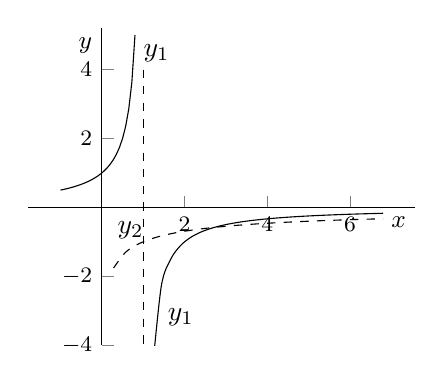
\begin{tikzpicture}
\begin{axis}[small,axis lines*=middle,ymin=-4,ymax=5.2,xlabel={$x$},ylabel={$y$},xlabel style={at={(current axis.right of origin)},anchor=north east},ylabel style={rotate=-90},ylabel style={at={(current axis.above origin)},anchor=north east}]
\addplot[domain=-1:0.8]{1/(1-x)}node[pos=0.9,right]{$y_1$};
\addplot[domain=1.2:6.8,smooth]{1/(1-x)}node[pos=0.2,right]{$y_1$};
\addplot[dashed,domain=0:6.8,smooth]{ln(x)/(1-x)}node[pos=0.1,above]{$y_2$};
\addplot[dashed] plot coordinates {(1,4) (1,-4)};
\end{axis}
\end{tikzpicture}
\caption{مثال \حوالہ{مثال_بیسل_دوسری_صورت_دوہرا_حل} کے حل۔}
\label{شکل_مثال_بیسل_دوسری_صورت_دوہرا_حل}
\end{figure} 
\انتہا{مثال}
%======================
\ابتدا{مثال}\quad لوگارتھمی جزو والا دوسرا حل\\
درج ذیل سادہ تفرقی مساوات حل کریں۔
\begin{align}\label{مساوات_بیسل_لوگارتھمی_جزو_الف}
(x^2-x)y''-xy'+y=0
\end{align}

حل: مساوات \حوالہ{مساوات_طاقتی_فروبنیوس_ب} اور اس کے تفرقات مساوات \حوالہ{مساوات_بیسل_اشاری_تفرقات} کو مساوات \حوالہ{مساوات_بیسل_لوگارتھمی_جزو_الف} میں پر کرتے ہیں۔
\begin{multline*}
(x^2-x)\sum_{m=0}^{\infty} (m+r)(m+r-1)a_mx^{m+r-2}-x\sum_{m=0}^{\infty}(m+r)a_m x^{m+r-1}\\
+\sum_{m=0}^{\infty} a_mx^{m+r}=0
\end{multline*}
\عددی{x^2}  اور \عددی{x} کو مجموعوں کے اندر لے جاتے ہوئے اور \عددی{x} کی یکساں طاقتوں کا اکٹھے کرتے ہوئے درج ذیل ملتا ہے۔
\begin{align}\label{مساوات_بیسل_تیسری_صورت_الف}
\sum_{m=0}^{\infty} (m+r-1)^2a_mx^{m+r}-\sum_{m=0}^{\infty} (m+r)(m+r-1)a_mx^{m+r-1}=0
\end{align}
\عددی{x} کی کم تر طاقت \عددی{x^{r-1}}، جو \عددی{m=0}  پر کرنے سے دوسرے مجموعے سے ملتا ہے، کے عددی سر کو صفر کے برابر پر کرنے سے
\begin{align*}
r(r-1)=1
\end{align*}
یعنی \عددی{r_1=1} اور \عددی{r_2=0} ملتے ہیں (جذر یوں لکھے جاتے ہیں کہ \عددی{r_1-r_2>0} ہو۔) جن میں فرق عدد صحیح کے برابر  ہے لہٰذا یہ تیسری صورت ہے۔

\موٹا{پہلا حل}:مساوات \حوالہ{مساوات_بیسل_تیسری_صورت_الف} کو یکساں طاقت کی صورت میں لکھنے کی خاطر پہلے مجموعے میں \عددی{m=s} اور دوسرے مجموعے میں \عددی{s=m-1} یعنی \عددی{m=s+1} پر کرتے ہیں۔
 \begin{align}
\sum_{s=0}^{\infty} (s+r-1)^2a_sx^{s+r}-\sum_{s=-1}^{\infty} (s+r+1)(s+r)a_{s+1}x^{s+r}=0
\end{align}
\عددی{x^{s+r}} کے عددی سروں کے مجموعے کو صفر کے برابر پر کرتے ہوئے
\begin{align*}
a_{s+1}=\frac{(s+r-1)^2}{(s+r+1)(s+r)}a_s
\end{align*}
ملتا ہے جس میں \عددی{r=1} پر کرتے ہوئے 
\begin{align}
a_{s+1}=\frac{s^2}{(s+2)(s+1)}a_s\quad \quad (s=0,1,\cdots)
\end{align}
حاصل ہوتا ہے  جس سے \عددی{a_1=0}، \عددی{a_2=0}، \نقطے حاصل ہوتے ہیں۔یوں \عددی{a_0=1} چنتے ہوئے پہلا حل \عددی{y_1=a_0x^{r_1}=x} ملتا ہے۔

\موٹا{دوسرا حل}:ترکیب تخفیف درجہ (حصہ \حوالہ{حصہ_دوسری_متجانس_خطی_دو_درجی}) استعمال کرتے ہوئے \عددی{y_2=uy_1=xu} لیتے ہیں۔اس طرح \عددی{y_2'=u+u'x} اور \عددی{y_2''=xu''+2u'} ہوں گے۔انہیں دیے گئے تفرقی مساوات میں پر کرتے ہیں۔
\begin{align*}
(x^2-x)(xu''+2u')-x(xu'+u)+xu=0
\end{align*}
اس میں \عددی{xu} کٹ جاتا ہے۔بقایا مساوات کو \عددی{x} سے تقسیم کرتے ہوئے ترتیب دیتے ہیں۔
\begin{align*}
(x^2-x)u''+(x-2)u'=0
\end{align*}
اس کو جزوی کسری پھیلاو کی مدد سے لکھتے ہوئے تکمل لیتے ہیں۔(تکمل کا مستقل صفر چننا گیا ہے۔)
\begin{align*}
\frac{u''}{u'}=-\frac{x-2}{x^2-x}=-\frac{2}{x}+\frac{1}{1-x}\,,\quad \ln u'=\ln \abs{\frac{x-1}{x^2}}
\end{align*}
اس کو قوت نمائی طور پر لکھتے ہوئے تکمل لیتے ہیں۔(تکمل کا مستقل صفر چنتے ہیں۔)
\begin{align*}
u'=\frac{x-1}{x^2}=\frac{1}{x}-\frac{1}{x^2}, \quad u=\ln x+\frac{1}{x}, \quad y_2=uy_1=x\ln x+1
\end{align*}
\عددی{y_1} اور \عددی{y_2} خطی طور غیر تابع ہیں اور \عددی{y_2} میں لوگارتھمی جزو پایا جاتا ہے۔یوں مثبت \عددی{x} پر یہ حل کی اساس ہیں۔
\انتہا{مثال}
%======================

ترکیب فروبنیوس سے \اصطلاح{بیش ہندسی مساوات} حل ہوتا ہے جس کے حل میں کئی اہم تفاعل شامل ہیں۔بعض اوقات دیے گئے مساوات کو مساوات \حوالہ{مساوات_طاقتی_فروبنیوس_الف} کی صورت میں لانے میں دشواری پیش آتی ہے۔یوں 
\begin{align*}
x(x-1)y''+(3x-1)y'+y=0
\end{align*}
کو \عددی{x(x-1)} سے تقسیم کرتے ہوئے  \عددی{y''+\tfrac{3x-1}{x(x-1)}y'+\tfrac{1}{x(x-1)}y=0} ملتا ہے جس کے آخری جزو کو \عددی{\tfrac{x}{x}} سے ضرب دیتے ہوئے \عددی{y''+\tfrac{3x-1}{x(x-1)}y'+\tfrac{x}{x^2(x-1)}y=0} ملتا ہے جو درکار صورت ہے جس میں \عددی{p=\tfrac{3x-1}{x-1}} اور \عددی{q=\tfrac{x}{x-1}} ہیں۔ 

ترکیب فروبنیوس کو استعمال کرتے ہوئے عموماً اتنا کافی ہوتا ہے کہ مساوات کو \عددی{a(x)y''+b(x)y'+c(x)y=0} شکل میں لایا جائے۔ درج ذیل سوالات حل کرتے ہوئے ایسا ہی کریں۔

مسئلہ \حوالہ{مسئلہ_طاقتی_فروبنیوس} میں \عددی{x} کی جگہ \عددی{x-x_0} بھی ممکن ہے جہاں \عددی{x_0} مساوات کا نادر نقطہ ہے۔یوں عمومی تفرقی مساوات 
\begin{align}\label{مساوات_بیسل_عمومی_ترکیب_فروبنیوس}
(x-x_0)^2 \alpha(x) y'' +(x-x_0)\beta(x)y'+\gamma(x)y=0
\end{align}
جس میں  \عددی{\alpha(x)}، \عددی{\beta(x)} اور \عددی{\gamma(x)} تحلیلی ہوں (لہٰذا انہیں درج لکھا جا سکتا ہے) 
\begin{align*}
\alpha=\alpha_0+\alpha_1x+\cdots,\quad \beta=\beta_0+\beta_1x+\cdots, \quad \gamma=\gamma_0+\gamma_1x+\cdots
\end{align*}
کو ترکیب فروبنیوس سے حل کرتے ہوئے اشاری مساوات
\begin{align}
\alpha_0 r^2+(\beta_0-\alpha_0)r+\gamma_0=0
\end{align}
حاصل ہو گی۔مساوات \حوالہ{مساوات_بیسل_عمومی_ترکیب_فروبنیوس} کو \عددی{\alpha(x)} سے تقسیم کرتے ہوئے مساوات \حوالہ{مساوات_طاقتی_فروبنیوس_الف} طرز کی مساوات حاصل ہوتی ہے۔آپ دیکھ سکتے ہیں کہ مساوات \حوالہ{مساوات_بیسل_عمومی_ترکیب_فروبنیوس} میں \عددی{x_0=0} پر کرنے سے  مساوات \حوالہ{مساوات_طاقتی_فروبنیوس_الف} حاصل ہوتی ہے۔مساوات \حوالہ{مساوات_بیسل_عمومی_ترکیب_فروبنیوس} کا حل
\begin{align}
y=x^r\sum_{m=0}^{\infty} c_m (x-x_0)^m
\end{align}
لکھ کر حاصل کیا جائے گا۔
%======================
\ابتدا{مثال}\شناخت{مثال_بیسل_دوسرا_حل_کیوں_نہیں_حاصل_ہوتا}\quad تیسری صورت میں بعض اوقات \عددی{r_2} سے حل نہیں لکھا جا سکتا ہے۔\\
اشاری مساوات کے جذر میں فرق عدد صحیح ہونے کی صورت میں کبھی کبھار دوسرا حل \عددی{y_2=x^{r_2}\sum c_m x^m} نہیں لکھا جا سکتا ہے۔اس مثال میں اس بات کی وضاحت ہو گی۔آئیں درج ذیل مساوات کو حل کرتے ہیں۔
\begin{align*}
2xy''-4y'-y=0
\end{align*}
اس مساوات میں \عددی{y=x^r\sum_{m=0}^{\infty}c_mx^m=\sum_{m=0}^{\infty}c_mx^{m+r}} اور اس کے تفرقات
\begin{align*}
y'=\sum_{m=0}^{\infty} (m+r)c_mx^{m+r-1},\quad y''=\sum_{m=0}^{\infty} (m+r)(m+r-1)c_mx^{m+r-2}
\end{align*}
پر کرتے ہوئے
\begin{align*}
2x\sum_{m=0}^{\infty} (m+r)(m+r-1)c_mx^{m+r-2}-4\sum_{m=0}^{\infty}(m+r)c_mx^{m+r-1}-\sum_{m=0}^{\infty}c_mx^{m+r}=0
\end{align*}
یعنی
\begin{align*}
\sum_{m=0}^{\infty}2 (m+r)(m+r-1)c_mx^{m+r-1}-\sum_{m=0}^{\infty}4(m+r)c_mx^{m+r-1}-\sum_{m=0}^{\infty}c_mx^{m+r}=0
\end{align*}
ملتا ہے۔تینوں مجموعوں سے \عددی{x^{r-1}} باہر نکالتے ہوئے کاٹتے ہیں۔
\begin{align*}
x^{r-1}\sum_{m=0}^{\infty}2 (m+r)(m+r-1)c_mx^{m}-\sum_{m=0}^{\infty}4(m+r)c_mx^{m}-\sum_{m=0}^{\infty}c_mx^{m+1}=0
\end{align*}
پہلے اور دوسرے مجموعے میں \عددی{s=m} اور تیسرے مجموعے میں \عددی{s=m+1} پر کرتے ہیں تا کہ \عددی{x} کے تمام طاقت یکساں لکھیں جائیں۔
\begin{align*}
\sum_{s=0}^{\infty}2 (s+r)(s+r-1)c_sx^{s}-\sum_{s=0}^{\infty}4(s+r)c_sx^{s}-\sum_{s=1}^{\infty}c_{s-1}x^{s}=0
\end{align*}
آپ نے دیکھا کہ تیسرے مجموعے کا پہلا رکن اب \عددی{s=1} سے ظاہر کیا جائے گا۔پہلے دو مجموعوں کا پہلا پہلا رکن مجموعے کے باہر لکھتے ہیں تا کہ تمام مجموعوں کا پہلا رکن ایک ہی جگہ سے شروع ہو۔ 
\begin{multline*}
2(0+r)(0+r-1)c_0x^0+\sum_{s=1}^{\infty}2 (s+r)(s+r-1)c_sx^{s}\\
-4(0+r)c_0x^0-\sum_{s=1}^{\infty}4(s+r)c_sx^{s}-\sum_{s=1}^{\infty}c_{s-1}x^{s}=0
\end{multline*}
یوں تمام مجموعوں کا پہلا رکن \عددی{s=1} ظاہر کرے گا۔تینوں مجموعوں کو اکٹھا لکھتے ہیں
\begin{multline}\label{مساوات_بیسل_اشاری_عمومی_الف}
\underbrace{[2r(r-1)-4r]}_{2r(r-3)}c_0+\sum_{s=1}^{\infty}[2 (s+r)(s+r-1)c_s-4(s+r)c_s-c_{s-1}]x^{s}=0
\end{multline}
جہاں پہلا رکن  اشاری مساوات \عددی{2r(r-3)=0} دیتا ہے جس کے جذر \عددی{r_1=3} اور \عددی{r_2=0} ہیں۔(یاد رہے کہ بڑی مقدار کے جذر کو \عددی{r_1} لکھا جاتا ہے اور اسی کی مدد سے پہلا حل حاصل کیا جاتا ہے۔)

مساوات \حوالہ{مساوات_بیسل_اشاری_عمومی_الف} میں \عددی{r=r_1=3} پر کرتے ہوئے
 \begin{align*}
[2\cdot 3(3-1)-4\cdot 3]c_0+\sum_{s=1}^{\infty}[2 (s+3)(s+3-1)c_s-4(s+3)c_s-c_{s-1}]x^{s}=0
\end{align*}
یعنی
 \begin{align*}
\sum_{s=1}^{\infty}[2s(s+3)c_s-c_{s-1}]x^{s}=0
\end{align*}
ملتا ہے جس سے درج ذیل کلیہ توالی لکھی جا سکتا ہے۔
\begin{align*}
c_s=\frac{1}{2s(s+3)}c_{s-1}\quad \quad (s\ge 1)
\end{align*}
اس کو استعمال کرتے ہوئے عددی سر حاصل کرتے ہیں۔
\begin{align*}
c_1&=\frac{1}{2\cdot 1(1+3)}c_0=\frac{1}{2\cdot 1 (4)}c_0\\
c_2&=\frac{1}{2\cdot 2(2+3)}c_1=\frac{1}{2\cdot 2(2+3)}\cdot \frac{1}{2\cdot 1 (4)}c_0=\frac{1}{2^2(2\cdot 1)(5\cdot 4)}c_0\\
&=\frac{3\cdot 2\cdot 1}{2^2(2\cdot 1)(5\cdot 4\cdot 3\cdot 2\cdot 1)}c_0=\frac{6}{2^2(2\cdot 1)(5\cdot 4\cdot 3\cdot 2\cdot 1)}c_0\\
c_3&=\frac{1}{2\cdot 3(3+3)}c_2=\frac{1}{2\cdot 3(6)}\cdot \frac{6}{2^2(2\cdot 1)(5\cdot 4\cdot 3\cdot 2\cdot 1)}c_0\\
&=\frac{6}{2^3(3\cdot 2\cdot 1)(6\cdot 5\cdot 4\cdot 3\cdot 2\cdot 1)}c_0\\
&\vdots\\
c_s&=\frac{6}{2^s s!(s+3)!}c_0
\end{align*}
آپ دیکھ سکتے ہیں کہ یہ آخری کلیہ \عددی{s=0} اور \عددی{s=1} کے لئے بھی کار آمد ہے لہٰذا ہم عمومی کلیہ توالی
\begin{align*}
c_s&=\frac{6}{2^s s!(s+3)!}c_0\quad \quad (s=0,1,2,\cdots)
\end{align*}
اور پہلا حل
\begin{align*}
y_1=x^{r_1}\sum_{m=0}^{\infty}\frac{6}{2^m m!(m+3)!}c_0x^m=c_0x^3\sum_{m=0}^{\infty}\frac{6}{2^m m!(m+3)!}x^m
\end{align*}
لکھ سکتے ہیں۔

آئیں \عددی{r=r_2=0} کو استعمال کرتے ہوئے دوسرا حل حاصل کرنے کی کوشش کریں۔  مساوات \حوالہ{مساوات_بیسل_اشاری_عمومی_الف} میں \عددی{r=0} پر کرتے ہوئے
\begin{multline*}
[2\cdot 0(0-1)-4\cdot 0]c_0+\sum_{s=1}^{\infty}[2 (s+0)(s+0-1)c_s-4(s+0)c_s-c_{s-1}]x^{s}=0
\end{multline*}
ملتا ہے جس میں \عددی{c_0} کا عددی سر صفر کے برابر ہے جبکہ \عددی{x_s} کے عددی سر سے درج ذیل کلیہ توالی لکھا جا سکتا ہے۔
\begin{align*}
c_s=\frac{1}{2s(s-3)}c_{s-1}
\end{align*}
اس کلیہ توالی کو استعمال کرتے ہوئے عددی سر حاصل کرتے ہیں۔
\begin{align*}
c_1&=\frac{1}{2\cdot 1(1-3)}c_0\\
c_2&=\frac{1}{2\cdot 2(2-3)}c_1=\frac{1}{2\cdot 2(2-3)}\frac{1}{2\cdot 1(1-3)}c_0\\
c_3&=\frac{1}{2\cdot 3\underbrace{(3-3)}_{=0}}c_2=\frac{1}{2\cdot 3(3-3)}\frac{1}{2\cdot 2(2-3)}\frac{1}{2\cdot 1(1-3)}c_0=\frac{c_0}{0}
\end{align*}
ہم دیکھتے ہیں کہ \عددی{c_0 \ne 0} کی صورت میں \عددی{c_3 =\infty} حاصل ہوتا ہے جبکہ \عددی{c_0} صفر نہیں ہو سکتا۔ایسا ہونے سے تمام عددی سر صفر کے برابر حاصل ہوتے ہیں جو \عددی{y_2=0} دیگا۔اشاری مساوات کے جذر میں فرق عدد صحیح ہونے کی صورت میں ہر بار ایک عددی سر \عددی{\tfrac{c_0}{0}} حاصل ہو گا جس کی بنا چھوٹا جذر استعمال کرتے ہوئے دوسرا حل حاصل نہیں کیا جا سکتا ہے۔
\انتہا{مثال}
%================
\حصہء{سوالات}

سوال \حوالہ{سوال_بیسل_فروبنیوس_الف} تا سوال \حوالہ{سوال_بیسل_فروبنیوس_ب} کی اساس کو ترکیب فروبنیوس سے حاصل کریں۔ حاصل تسلسل کو بطور تفاعل پہچاننے کی کوشش کریں۔\\

%============
\ابتدا{سوال}\شناخت{سوال_بیسل_فروبنیوس_الف}\quad
$x^2y''+4xy'+(x^2+2)y=0$\\
جواب:\عددی{y_1=x^{-1}(1-\tfrac{x^2}{3!}+\tfrac{x^4}{5!}-+\cdots)}، \عددی{y_2=x^{-1}(x-\tfrac{x^3}{12}+\tfrac{x^5}{360}-+\cdots)}
\انتہا{سوال}
%==================
\ابتدا{سوال}\quad
$xy''+2y'+xy=0$\\
جواب:\عددی{y_1=1-\tfrac{x^2}{3!}+\tfrac{x^4}{5!}-+\cdots=\tfrac{\sin x}{x}}، \عددی{y_2=\tfrac{1}{x}-\tfrac{x}{2!}+\tfrac{x^3}{4!}-\cdots=\tfrac{\cos x}{x}}
\انتہا{سوال}
%=================
\ابتدا{سوال}\quad 
$(x-1)^2y''-2(x-1)y'+2y=0$\\
جواب:اس طرز کے مساوات میں بہتر ہوتا ہے کہ \عددی{X=x-x_0=x-1} اور \عددی{Y(X)} استعمال کیا جائے جس سے درج بالا مساوات \عددی{X^2Y''-2XY'+2Y=0} لکھی جاتی ہے۔حل کرنے کے بعد واپس \عددی{x} کا استعمال کریں۔ 
\عددی{r_1=2}، \عددی{r_2=1} ہیں۔\عددی{r=r_1=2} استعمال کرتے ہوئے تمام عددی سر صفر کے برابر حاصل ہوتے ہیں جبکہ \عددی{r=r_2=1} استعمال کرتے ہوئے حل \عددی{y=(x-1)^1[c_0+c_1(x-1)]} ملتا ہے جس میں دو عدد اختیاری مستقل ہیں لہٰذا یہ عمومی حل ہے۔یوں اساس \عددی{y_1=x-1} اور \عددی{y_2=(x-1)^2} ہے۔
\انتہا{سوال}
%==================
\ابتدا{سوال}\quad
$y''+xy'+(1-\frac{2}{x^2})y=0$\\
جواب:\عددی{r_1=0} \عددی{r_2=-3} ہیں جن میں عددی صحیح فرق پایا جاتا ہے جو تیسری صورت ہے۔یوں \عددی{r_1} استعمال کرتے ہوئے   \عددی{y_1=c_2(x^2-\tfrac{3}{10}x^4+\tfrac{3}{56}x^6-\tfrac{1}{144}x^8+\cdots)} حاصل ہوتا ہے جبکہ \عددی{r_2} استعمال کرتے ہوئے \عددی{y_2=c_2x^{-1}} حاصل ہوتا ہے۔
\انتہا{سوال}
%===================
\ابتدا{سوال}\شناخت{سوال_بیسل_جواب_کا_حصہ_رد}\quad
$xy''+3y'+4x^3y=0$\\
جواب:\عددی{r_1=0} اور \عددی{r_2=-2} ہیں۔ \عددی{r_1} کو استعمال کرتے ہوئے
\begin{align*}
y_1=x^{0}(1-\tfrac{1}{6}x^4+\tfrac{1}{120}x^8+\cdots)=\tfrac{\sin x^2}{x^2}
\end{align*}
ملتا ہے جبکہ \عددی{r_2} کو استعمال کرتے ہوئے
\begin{align*}
y^*_2=c_0(\frac{1}{x^2}-\frac{x^2}{2}+\frac{x^6}{24}+\cdots)+c_2(1-\frac{x^4}{6}+\frac{x^8}{120}-\cdots)
\end{align*}
ملتا ہے جہاں آخری قوسین در حقیقت \عددی{y_1} ہی ہے لہٰذا اساس لکھتے ہوئے اس حصے کو رد کیا جاتا ہے۔اس طرح اساس درج ذیل ہو گا۔
\begin{align*}
y_1&=1-\tfrac{1}{6}x^4+\tfrac{1}{120}x^8+\cdots=\tfrac{\sin x^2}{x^2}\\
y_2&=\frac{1}{x^2}-\tfrac{1}{2}x^2+\tfrac{1}{24}x^6+\cdots=\tfrac{\cos x^2}{x^2}
\end{align*}
\انتہا{سوال}
%====================
\ابتدا{سوال}\quad
$x^2y''-5xy'+9y=0$\\
جواب:\عددی{r_1=r_2=3} ہے جو دوسری صورت ہے۔یوں پہلا حل  \عددی{y_1=x^3} ملتا ہے جبکہ دوسرا حل بذریعہ تخفیف درجہ (\عددی{y_2=x^3u} پر کرتے ہوئے) \عددی{y_2=x^3\ln x} حاصل ہوتا ہے۔ 
\انتہا{سوال}
%======================
\ابتدا{سوال}\quad
$xy''+y'-xy=0$\\
جواب:\عددی{r_1=r_2=0} ملتا ہے۔\عددی{y_1=1+\tfrac{x^2}{4}+\tfrac{x^4}{64}+\tfrac{x^6}{2304}+\cdots}، \\
\عددی{y_2=y_1\ln x-\tfrac{x^2}{4}-\tfrac{3x^4}{8\cdot 16}-\cdots}
\انتہا{سوال}
%===================
\ابتدا{سوال}\quad
$x^2y''+xy'-4y=0$\\
جواب:\عددی{r_1=2}، \عددی{r_2=-2} میں فرق عدد صحیح ہے۔\عددی{r_1} کو استعمال کرتے ہوئے \عددی{y_1=x^2} ملتا ہے۔اگر آپ \عددی{r_2} کو استعمال کرتے ہوئے  \عددی{y_1} کی طرز کا حل حاصل کرنا چاہیں تو آپ کو \عددی{y_2=x^{-2}(c_0+c_4x^4)=c_0x^{-2}+c_4x^2} ملتا ہے جس میں \عددی{x^2} درحقیقت \عددی{y_1} ہے جسے رد کرتے ہوئے اساس میں \عددی{y_2=\tfrac{1}{x^2}} لکھا جائے گا۔  
\انتہا{سوال}
%================
\ابتدا{سوال}\quad
$x^2y''+6xy'+(6-4x^2)y=0$\\
جواب:\عددی{r_1=-2}، \عددی{r_2=-3} ہیں۔ \عددی{r_1} سے \عددی{y_1=\tfrac{2}{3}+\tfrac{1}{x^2}+\tfrac{2}{15}x^2+\cdots=\tfrac{\sinh 2x}{2x^3}}  حاصل ہوتا ہے جبکہ \عددی{r_2} سے \عددی{y=c_0(\tfrac{1}{x^3}+\tfrac{2}{x}+\tfrac{2}{3}x+\cdots)+c_1y_1} ملتا ہے لہٰذا \عددی{y_2=\tfrac{1}{x^3}+\tfrac{2}{x}+\tfrac{2}{3}x+\cdots} لکھا جائے گا یعنی \عددی{y_2=\tfrac{\cosh 2x}{x^3}} ہے۔
\انتہا{سوال}
%====================
\ابتدا{سوال}\quad
$xy''+(1-2x)y'+(x-1)y=0$\\
جواب:\عددی{r_1=r_2=0} ہے جو دوسری صورت ہے۔ اساس \عددی{y_1=1+x+\tfrac{x^2}{2!}+\tfrac{x^3}{3!}+\tfrac{x^4}{4!}+\cdots=e^x} اور \عددی{y_2=e^x \ln x} ہیں۔
\انتہا{سوال}
%===================
\ابتدا{سوال}\quad
$xy''+(2x+1)y'+(x+1)y=0$\\
جواب:\عددی{r_1=r_2=0} جبکہ \عددی{y_1=e^{-x}} اور \عددی{y_2=e^{-x}\ln x} ہیں۔
\انتہا{سوال}
%===================
\ابتدا{سوال}\quad 
$y''+(x-1)y=0$\\
جواب:\عددی{r_1=} اور \عددی{r_2=-1} ہیں۔ \عددی{r_1} سے ایسا تسلسل ملتا ہے جس میں دو عدد اختیاری مستقل پائے جاتے ہیں لہٰذا اس تسلسل کو دو عدد تفاعل میں لکھتے ہوئے اساس \عددی{y_1=1+\tfrac{x^2}{2}-\tfrac{x^3}{6}+\tfrac{x^4}{24}-\tfrac{x^5}{30}+\cdots} اور 
\عددی{y_2=x+\tfrac{x^3}{6}-\tfrac{x^4}{12}+\tfrac{x^5}{120}-\cdots} حاصل ہوتی ہے۔
\انتہا{سوال}
%===================
\ابتدا{سوال}\شناخت{سوال_بیسل_فروبنیوس_ب}\quad
$xy''+(2-2x)y'+(x-2)y=0$\\
جواب:\عددی{r_1=0} اور \عددی{r_2=-1} ہیں۔\عددی{r_1} استعمال کرتے ہوئے  \عددی{y_1=1+x+\tfrac{x^2}{2}+\tfrac{x^3}{6}+\cdots=e^x} ملتا ہے۔دوسرا حل \عددی{y_2=uy_1} لکھ کر تخفیف درجی کے استعمال سے \عددی{y_2=\tfrac{e^x}{x}} حاصل ہوتا ہے۔
\انتہا{سوال}
%===================
\ابتدا{سوال}\شناخت{سوال_بیسل_بیش_ہندسی_الف}\quad \اصطلاح{گاوس بیش ہندسی مساوات}\\
درج ذیل تفرقی مساوات
\begin{align}\label{مساوات_بیسل_بیش_ہندسی_الف}
x(1-x)y''+[c-(a+b+1)x]y'-aby=0
\end{align}
جہاں \عددی{a}، \عددی{b} اور \عددی{c} مستقل ہیں \اصطلاح{گاوس بیش ہندسی مساوات}\فرہنگ{گاوس بیش ہندسی مساوات}\فرہنگ{مساوات!گاوس بیش ہندسی}\فرہنگ{بیش ہندسی!گاوس}\حاشیہب{Gauss' hypergeometric equation}\فرہنگ{Gauss' hypergeometric equation} کہلاتی ہے۔ثابت کریں کہ اس کی اشاری مساوات کے جذر \عددی{r_1=0} اور \عددی{r_2=1-c} ہیں۔ثابت کریں کہ \عددی{r=r_1=0} کے لئے ترکیب فروبنیوس کے استعمال سے درج ذیل حل ملتا ہے جہاں \عددی{c \ne 0,-1,-2,\cdots} ہے۔
\begin{align}\label{مساوات_بیسل_بیش_ہندسی_حل_الف}
y_1(x)=1+\frac{ab}{1! c}x+\frac{a(a+1)b(b+1)}{2!c(c+1)}x^2+\frac{a(a+1)(a+2)b(b+1)(b+2)}{3!c(c+1)(c+2)}x^3+\cdots
\end{align}
یہ تسلسل \اصطلاح{بیش ہندسی تسلسل}\فرہنگ{بیش ہندسی تسلسل}\حاشیہب{hypergeometric series}\فرہنگ{hypergeomitric!series} کہلاتی ہے جس کا مجموعہ عموماً \عددی{F(a,b,c;x)} لکھا اور \اصطلاح{بیش ہندسی تفاعل}\فرہنگ{بیش ہندسی تفاعل}\حاشیہب{hypergeomitric function}\فرہنگ{hypergeometric function} پکارا جاتا ہے۔
\انتہا{سوال}
%=======================
\ابتدا{سوال}
ثابت کریں کہ \عددی{\abs{x} <1} کے لئے تسلسل \حوالہ{مساوات_بیسل_بیش_ہندسی_حل_الف}  مرتکز ہے۔

جواب:$\lim_{m\to \infty}\abs{\tfrac{a_{m+1}}{a_m}}=\lim_{m\to \infty}\abs{\tfrac{(a+m)(b+m)}{(m+1)!(c+m)}\tfrac{m!(c+m-1)}{(1+m-1)(b+m-1)}}=1$ ہے لہٰذا \عددی{R<1} ہو گا۔
\انتہا{سوال}
%======================
\ابتدا{سوال}
بیش ہندسی تفرقی مساوات کا حل مساوات \حوالہ{مساوات_بیسل_بیش_ہندسی_حل_الف} مستقل \عددی{a} اور \عددی{b} کی کن قیمتوں پر کثیر رکنی کی صورت اختیار کرے گا۔ 

جواب:\عددی{a=0,-1,-2,-\cdots} اور \عددی{b=0,-1,-2,-\cdots}
\انتہا{سوال}
%=====================
\ابتدا{سوال}
\عددی{a=b=c=1} کی صورت میں  تسلسل \حوالہ{مساوات_بیسل_بیش_ہندسی_حل_الف} سے \اصطلاح{ہندسی تسلسل}\فرہنگ{ہندسی تسلسل}\حاشیہب{geometric series}\فرہنگ{geometric series} حاصل کریں۔

جواب:\عددی{F(1,1,1;x)=1+x+x^2+x^3+\cdots=\frac{1}{1-x}}
\انتہا{سوال}
%=====================
\ابتدا{سوال}
ثابت کریں کہ \عددی{F(1,1,1;x)=F(1,b,b;x)=F(a,1,a;x)} یعنی ہندسی تسلسل ہے۔اسی سے تفاعل \عددی{F(a,b,c;x)} کا نام بیش ہندسی تفاعل نکلا ہے۔
\انتہا{سوال}
%===================
\ابتدا{سوال}
ثابت کریں کہ سوال \حوالہ{سوال_بیسل_بیش_ہندسی_الف} میں \عددی{r_2=1-c} استعمال کرتے ہوئے مساوات \حوالہ{مساوات_بیسل_بیش_ہندسی_الف} کا دوسرا حل درج ذیل حاصل ہوتا ہے جہاں \عددی{c \ne 2,3,4,7\cdots} ہے۔
\begin{multline}\label{مساوات_بیسل_بیش_ہندسی_حل_ب}
y_2(x)=x^{1-c}\left(1+\frac{(a-c+1)(b-c+1)}{1!(-c+2)}x\right.\\
\left.+\frac{(a-c+1)(a-c+2)(b-c+1)(b-c+2)}{2!(-c+2)(-c+3)}x^2+\cdots\right)
\end{multline}
\انتہا{سوال}
%=================
\ابتدا{سوال}
ثابت کریں کہ مساوات \حوالہ{مساوات_بیسل_بیش_ہندسی_حل_ب} کو درج ذیل لکھا جا سکتا ہے۔
\begin{align}\label{مساوات_بیسل_بیش_ہندسی_حل_پ}
y_2(x)=x^{1-c}F(a-c+a,b-c+1,2-c;x)
\end{align}
\انتہا{سوال}
%==================
\ابتدا{سوال}
ثابت کریں کہ \عددی{c\ne 0, \mp 1,\mp2,\mp 3\mp\cdots} کی صورت میں مساوات \حوالہ{مساوات_بیسل_بیش_ہندسی_الف} کے حل کی اساس مساوات \حوالہ{مساوات_بیسل_بیش_ہندسی_حل_الف} اور مساوات \حوالہ{مساوات_بیسل_بیش_ہندسی_حل_ب} ہیں۔
\انتہا{سوال}
%==================
\ابتدا{سوال}
درج ذیل ثابت کریں۔
\begin{align*}
(1+x)^n&=F(-n,b,b;-x)\\
(1-x^n)&=1-nxF(1-n,1,2;x)\\
\tan^{-1} x&=xF(\tfrac{1}{2},1,\tfrac{3}{2};-x^2)\\
\sin^{-1} x&=xF(\tfrac{1}{2},\tfrac{1}{2},\tfrac{3}{2};x^2)\\
\ln(1+x)&=xF(1,1,2;-x)\\
\ln \frac{1+x}{1-x}&=2xF(\tfrac{1}{2},1,\tfrac{3}{2};x^2)
\end{align*}
\انتہا{سوال}
%===================
\ابتدا{سوال}
درج ذیل مساوات میں \عددی{A}، \عددی{B}، \عددی{C}، \عددی{D} اور \عددی{K} مستقل ہیں، \عددی{\dot{y}} سے مراد \عددی{\tfrac{\dif y}{\dif t}} ہے  اور \عددی{t^2+At+B} کے منفرد جذر \عددی{t_1} اور \عددی{t_2} ہیں۔
\begin{align}
(t^2+At+B)\ddot{y}+(Ct+D)\dot{y}+Ky=0
\end{align}
اس مساوات میں  نیا متغیر \عددی{x=\tfrac{t-t_1}{t_2-t_1}} پر کرتے ہوئے بیش ہندسی مساوات حاصل کریں جس میں
\begin{align*}
Ct_1+D=-c(t_2-t_1), \quad C=a+b+1, \quad K=ab
\end{align*}
ہوں گے۔

جواب:چونکہ \عددی{t^2+At+B} کے منفرد (\عددی{t_2 \ne t_1}) جذر \عددی{t_1} اور \عددی{t_2} ہیں لہٰذا \عددی{t^2+At+B=(t-t_1)(t-t_2)} لکھا جا سکتا ہے۔اب نیا متغیرہ \عددی{x=\tfrac{t-t_1}{t_2-t_1}} لیتے ہوئے \عددی{t=(t_2-t_1)x+t_1} لکھا جا سکتا ہے۔یوں
\begin{align*}
t-t_1&=(t_2-t_1)x,\quad t-t_2=(t_2-t_1)(x-1),\\
(t-t_1)(t-t_2)&=(t_2-t_1)^2x(x-1),\quad \frac{\dif y}{\dif t}=\frac{1}{t_2-t_1}\frac{\dif y}{\dif x},\quad \frac{\dif^{\, 2} y}{\dif t^2}=\frac{1}{(t_2-t_1)^2}\frac{\dif^{\,2} y}{\dif x^2}
\end{align*}
ہوں گے جنہیں دیے گئے مساوات میں پر کرتے ہوئے
\begin{align}
x(1-x)y''-\left(\frac{Ct_1+D}{t_2-t_1}+Cx\right)y'-Ky=0
\end{align}
ملتا ہے۔
\انتہا{سوال}
%=====================
سوال \حوالہ{سوال_بیسل_بیش_ہندسی_تفرقی_الف} تا سوال \حوالہ{سوال_بیسل_بیش_ہندسی_تفرقی_ب} کے عمومی حل بیش ہندسی تفاعل کی صورت میں دریافت کریں۔

%====================
\ابتدا{سوال}\شناخت{سوال_بیسل_بیش_ہندسی_تفرقی_الف}\quad
$2x(1-x)y''-(1+5x)y'-y=0$\\
جواب:\عددی{y=c_1F(1,\tfrac{1}{2},-\tfrac{1}{2};x)+c_2x^{\tfrac{3}{2}}F(\tfrac{5}{2},2,\tfrac{5}{2};x)}
\انتہا{سوال}
%==================================
\ابتدا{سوال}\quad
$4(t^2-3t+2)\ddot{y}-2\dot{y}+y=0$\\
جواب:\عددی{y=c_1F(-\tfrac{1}{2},-\tfrac{1}{2},\tfrac{1}{2};t-1)+c_2(t-1)^{\tfrac{1}{2}}}
\انتہا{سوال}
%===========================
\ابتدا{سوال}\شناخت{سوال_بیسل_بیش_ہندسی_تفرقی_ب}\quad
$2(t^2-5t+6)\ddot{y}+(2t-3)\dot{y}-8y=0$\\
جواب:\عددی{y=c_1F(2,-2,-\tfrac{1}{2};t-2)+c_2(t-2)^{\tfrac{3}{2}}F(\tfrac{7}{2},-\tfrac{1}{2},\tfrac{5}{2};t-2)}
\انتہا{سوال}
%=======================================
%========================================

\حصہ{مساوات بیسل اور بیسل تفاعل}\شناخت{حصہ_طاقتی_بیسل_تفاعل}
اہم ترین سادہ تفرقی مساوات میں سے ایک \اصطلاح{بیسل مساوات}\فرہنگ{بیسل!مساوات}\فرہنگ{مساوات!بیسل}\حاشیہب{Bessel's equation}\فرہنگ{Bessel!equation}
\begin{align}\label{مساوات_بیسل_الف}
x^2y''+xy'+(x^2-\nu^2)y=0
\end{align}
ہے جہاں \عددیء{\nu}\حاشیہد{\عددی{\nu} یونانی حرف تہجی \اصطلاح{نی} ہے۔} حقیقی مستقل ہے جس کی قیمت صفر یا مثبت ہو گی۔یہ مساوات عموماً نلکی تشاکلی مسائل میں سامنے آتی ہے۔بیسل مساوات کو \عددی{x^2} سے تقسیم کرتے ہوئے معیاری صورت \عددی{y''+\tfrac{1}{x}y'+(\tfrac{x^2-\nu^2}{x^2})y=0} حاصل ہوتی ہے جو مسئلہ \حوالہ{مسئلہ_طاقتی_فروبنیوس} پر پورا اترتی ہے۔یوں بیسل مساوات کے حل کو ترکیب فروبنیوس سے درج ذیل لکھا جا سکتا ہے۔
\begin{align}\label{مساوات_بیسل_ب}
y=\sum_{m=0}^{\infty}c_mx^{m+r}\quad \quad (a_0 \ne 0)
\end{align}
مساوات \حوالہ{مساوات_بیسل_ب} اور اس کے ایک درجی اور دو درجی تفرقات کو مساوات \حوالہ{مساوات_بیسل_الف} میں پر کرتے ہیں۔
\begin{multline*}
\sum_{m=0}^{\infty}c_m(m+r)(m+r-1)x^{m+r}+\sum_{m=0}^{\infty}c_m(m+r)x^{m+r}+\sum_{m=0}^{\infty}c_mx^{m+r+2}\\
-\nu^2\sum_{m=0}^{\infty}c_mx^{m+r}=0
\end{multline*}
\عددی{x^{s+r}} کے عددی سروں کے مجموعے کو صفر کے برابر لکھتے ہوئے \عددی{c_0, c_1, \cdots} حاصل کرتے ہیں۔آپ دیکھ سکتے ہیں کہ \عددی{x^{s+r}} پہلے، دوسرے اور تیسرے مجموعوں میں \عددی{m=s} پر کرنے اور تیسرے مجموعے میں \عددی{m=s-2} پر کرنے سے ملتے ہیں۔یوں \عددی{s=0} اور \عددی{s=1} کی صورت میں تیسرا مجموعہ کوئی حصہ نہیں ڈالے گا جبکہ \عددی{s=2} کی صورت میں چاروں مجموعے حصہ ڈالیں گے۔یوں درج ذیل لکھا جا سکتا ہے۔
\begin{gather}
\begin{aligned}\label{مساوات_بیسل_پ}
r(r-1)a_0+ra_0-\nu^2a_0&=0\quad \quad (s=0)\\
(r+1)ra_1+(r+1)a_1-\nu^2a_1&=0\quad \quad (s=1)\\
(s+r)(s+r-1)a_s+(s+r)a_s+a_{s-2}-\nu^2a_s&=0\quad \quad (s=2,3,\cdots)
\end{aligned}
\end{gather}  
چونکہ \عددی{a_0 \ne 0} ہے لہٰذا مساوات \حوالہ{مساوات_بیسل_پ} کی پہلی مساوات  سے  \اصطلاح{اشاری مساوات} 
\begin{align}\label{مساوات_بیسل_ت}
(r+\nu)(r+\nu)=0
\end{align}
حاصل ہوتی ہے جس کے جذر \عددی{r_1=\nu (\ge 0)} اور \عددی{r_2=-\nu} ہیں۔

\جزوحصہء{توالی عددی سر؛ \عددی{r=r_1=\nu}}
دوسری مساوات \حوالہ{مساوات_بیسل_پ}  میں \عددی{r=\nu} پر کرتے ہوئے \عددی{(2\nu+1)a_1=0} ملتا ہے۔اب چونکہ \عددی{\nu} غیر منفی ہے لہٰذا \عددی{2\nu+1} صفر کے برابر نہیں ہو سکتا اور یوں \عددی{a_1=0} حاصل ہوتا ہے۔تیسری مساوات \حوالہ{مساوات_بیسل_پ}  میں \عددی{r=\nu} پر کرتے ہوئے درج ذیل ملتا ہے۔
\begin{align}\label{مساوات_بیسل_ٹ}
(s+2\nu)sa_s+a_{s-2}=0
\end{align}
چونکہ \عددی{a_1=0} اور \عددی{\nu\ge 0} ہے  لہٰذا مساوات \حوالہ{مساوات_بیسل_ٹ} سے \عددی{s_3=0}، \عددی{s_5=0}، \نقطے حاصل ہوتے ہیں۔ یوں تمام طاق عددی سر صفر کے برابر ہیں۔جفت عددی سر حاصل کرنے کی خاطر مساوات \حوالہ{مساوات_بیسل_ٹ} میں \عددی{s=2m} پر کرتے ہوئے
\begin{align*}
(2m+2\nu)2ma_{2m}+a_{2m-2}=0
\end{align*}
یعنی
\begin{align}\label{مساوات_بیسل_ث}
a_{2m}-\frac{1}{2^2m(\nu+m)}a_{2m-2},\quad \quad m=1,2,3,\cdots
\end{align}
ملتا ہے۔مساوات \حوالہ{مساوات_بیسل_ث} سے \عددی{c_2}، \عددی{c_4}، \نقطے لکھتے ہیں
\begin{align*}
a_2&=-\frac{a_0}{2^2(\nu+1)}\\
a_4&=-\frac{a_2}{2^2 2(\nu+2)}=\frac{a_0}{2^42!(\nu+1)(\nu+2)}
\end{align*}
اور یوں عمومی کلیہ 
\begin{align}\label{مساوات_بیسل_ج}
a_{2m}=\frac{(-1)^m a_0}{2^{2m}m!(\nu+1)(\nu+2)\cdots (\nu+m)},\quad \quad m=1,2,\cdots
\end{align}
حاصل ہوتا ہے۔

\جزوحصہء{عددی صحیح \عددی{\nu=n} کی صورت میں بیسل تفاعل \عددی{J_n(x)}}
\عددی{\nu} کی عدد صحیح قیمت کو روایتی طور پر \عددی{n} سے ظاہر کیا جاتا ہے۔یوں \عددی{\nu=n} کی صورت میں مساوات \حوالہ{مساوات_بیسل_ج}  درج ذیل لکھی جائے گی
\begin{align}\label{مساوات_بیسل_چ}
a_{2m}=\frac{(-1)^m a_0}{2^{2m}m!(n+1)(n+2)\cdots (n+m)},\quad \quad m=1,2,\cdots
\end{align}
جس میں \عددی{a_0} اختیاری مستقل ہے۔مساوات \حوالہ{مساوات_بیسل_چ} پر مبنی تسلسل میں بھی اختیاری مستقل \عددی{a_0} پایا جائے گا۔ہم اختیاری مستقل کی قیمت \عددی{a_0=1} چن سکتے ہیں البتہ اس سے بہتر قیمت 
\begin{align}\label{مساوات_بیسل_عددی_سر_الف}
a_0=\frac{1}{2^nn!}
\end{align}
ہے جس کو استعمال کرتے ہوئے مساوات \حوالہ{مساوات_بیسل_چ} کو
\begin{align*}
a_{2m}=\frac{(-1)^m}{2^{2m+n}m!n!(n+1)(n+2)\cdots (n+m)}
\end{align*}
یعنی
\begin{align}\label{مساوات_بیسل_ح}
a_{2m}=\frac{(-1)^m}{2^{2m+n}m!(n+m)!},\quad \quad m=1,2,\cdots
\end{align}
لکھا جا سکتا ہے۔آپ نے دیکھا کہ \عددی{a_0=\tfrac{1}{2^nn!}} چننے سے  بڑھتی ضربیہ \عددی{(n+1)(n+2)\cdots (n+m)} کو نہایت عمدگی کے ساتھ \اصطلاح{عدد ضربیہ}\فرہنگ{عدد ضربیہ}\حاشیہب{factorial}\فرہنگ{factorial} \عددی{(n+m)!} میں ضم کیا گیا ہے۔درج بالا عددی سر کو تسلسل\حوالہ{مساوات_بیسل_ب} میں پر کرتے ہوئے، اور یہ ذہن میں رکھتے ہوئے کہ \عددی{c_1=0}، \عددی{c_3=0}، \نقطے ہیں، بیسل مساوات \حوالہ{مساوات_بیسل_الف} کا مخصوص حل \عددی{J_n(x)}
\begin{align}\label{مساوات_بیسل_خ}
J_n(x)=x^n\sum_{m=0}^{\infty} \frac{(-1)^m x^{2m}}{2^{2m+n} m!(n+m)!} \quad \quad (n \ge 0)
\end{align}
ملتا ہے جو \اصطلاح{درجہ} \عددی{n} \اصطلاح{بیسل تفاعل کی پہلی قسم}\فرہنگ{بیسل!پہلی قسم درجہ \عددی{n}}\حاشیہب{Bessel function of the first kind of order n}\فرہنگ{Bessel!function, first kind}  کہلاتی ہے۔بیسل تفاعل \حوالہ{مساوات_بیسل_خ} تمام \عددی{x} کے لئے  مرتکز ہے یعنی (جیسا آپ عددی سر کی شرح \عددی{\tfrac{a_{m+1}}{a_m}} سے ثابت کر سکتے ہیں) اس کا رداس ارتکاز لامتناہی  \عددی{R =\infty} ہے۔یوں \عددی{J_n(x)} تمام \عددی{x} کے لئے معین ہے۔عددی سر کے نسب نما میں عدد ضربیہ \عددی{(n+m)!} کی بنا تسلسل بہت تیزی سے مرکوز ہوتی ہے۔
%=====================

\ابتدا{مثال}\quad بیسل تفاعل \عددی{J_0(x)} اور \عددی{J_1(x)}\\
مساوات \حوالہ{مساوات_بیسل_خ} میں \عددی{n=0} پر کرتے ہوئے \اصطلاح{درجہ \عددی{0} کا بیسل تفاعل} \عددی{J_0(x)}
\begin{align}\label{مساوات_بیسل_د}
J_0(x)=\sum_{m=0}^{\infty} \frac{(-1)^m x^{2m}}{2^{2m} (m!)^2} =1-\frac{x^2}{2^2(1!)^2}+\frac{x^4}{2^4(2!)^2}-\frac{x^6}{2^6(3!)^2}+-\cdots
\end{align}
حاصل ہوتا ہے (شکل \حوالہ{شکل_بیسل_تفاعل} دیکھیں) جو کوسائن تفاعل کی مانند ہے۔اسی طرح مساوات \حوالہ{مساوات_بیسل_خ} میں \عددی{n=1} پر کرتے ہوئے \اصطلاح{درجہ \عددی{1} کا بیسل تفاعل} \عددی{J_1(x)} 
\begin{align}\label{مساوات_بیسل_ڈ}
J_1(x)=\sum_{m=0}^{\infty} \frac{(-1)^m x^{2m+1}}{2^{2m+1} m!(m+1)!}=x-\frac{x^3}{2^31!2!}+\frac{x^5}{2^52!3!}-\frac{x^7}{2^73!4!}+-\cdots
\end{align}
حاصل ہوتا ہے  (شکل \حوالہ{شکل_بیسل_تفاعل} دیکھیں) جو سائن تفاعل کی مانند ہے لیکن جیسا آپ دیکھیں گے بیسل تفاعل کے صفر یکساں فاصلوں پر نہیں پائے جاتے ہیں اور \عددی{x} بڑھانے سے  تفاعل کا حیطہ کم ہوتا جاتا ہے۔
\begin{figure}
\centering
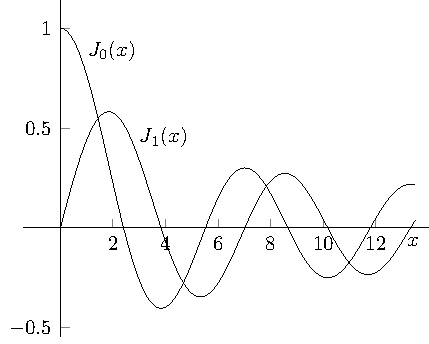
\includegraphics{figOctaveBesselFunction}
\caption{بیسل تفاعل کی پہلی قسم۔ \عددی{J_0}، \عددی{J_1}}
\label{شکل_بیسل_تفاعل}
\end{figure}
مساوات \حوالہ{مساوات_بیسل_الف} کو \عددی{x^2} سے تقسیم کرتے ہوئے  معیاری صورت \عددی{y''+\tfrac{1}{x}y'+(1-\tfrac{\nu^2}{x^2})y=0} ملتی ہے جس پر توجہ دیں۔ \عددی{x} کی زیادہ قیمت پر \عددی{\tfrac{1}{x}} اور \عددی{\tfrac{\nu^2}{x^2}} کو رد کرتے ہوئے بیسل مساوات سے \عددی{y''+y=0} حاصل ہوتا ہے جس کے حل \عددی{\cos x} اور \عددی{\sin x} ہیں۔آپ یہ بھی دیکھ سکتے ہیں کہ \عددی{\tfrac{y'}{x}} بطور تقصیری مستقل کردار ادا کرتے ہوئے بیسل تفاعل کا حیطہ گھٹانے میں مدد دے گی۔ زیادہ \عددی{x} کی صورت میں درج ذیل ثابت کیا جا سکتا ہے
\begin{align}\label{مساوات_بیسل_ذ}
J_n(x) \sim \sqrt{\frac{2}{\pi x}} \cos(x-\frac{n\pi}{2}-\frac{\pi}{4})
\end{align}
جہاں \عددی{\sim} کو \اصطلاح{متقاربی برابر}\فرہنگ{متقارب}\حاشیہب{asymptotically equal}\فرہنگ{asymptotically equal} پڑھیں اور جس کا مطلب ہے کہ کسی بھی قطعی \عددی{n} پر دونوں اطراف کی شرح، \عددی{x \to \infty} پر اکائی کے برابر ہو گی۔ 

مساوات \حوالہ{مساوات_بیسل_ذ} کم \عددی{x (>0)} کی صورت میں بھی بہترین ثابت ہوتی ہے۔اس کو استعمال کرتے ہوئے \عددی{J_0(x)} کے ابتدائی تین صفر \عددی{2.356}، \عددی{5.498} اور \عددی{8.639} حاصل ہوتے ہیں جبکہ ان کی حقیقی قیمتیں بالترتیب \عددی{2.405}، \عددی{5.520} اور \عددی{8.654} ہیں۔دونوں جوابات میں فرق \عددی{0.049}، \عددی{0.022} اور \عددی{0.015} ہے۔
\انتہا{مثال}
%=======================

\جزوحصہء{بیسل تفاعل جہاں \عددی{\nu \ge 0} کوئی بھی قیمت ہو سکتی ہے۔ گیما تفاعل}
گزشتہ حصے میں ہم نے عدد صحیح \عددی{\nu=n}کی صورت میں بیسل مساوات کا ایک حل دریافت کیا۔آئیں اب کسی بھی قیمت کے \عددی{\nu>0} کے لئے بیسل تفاعل کا عمومی حل تلاش کریں۔مساوات \حوالہ{مساوات_بیسل_عددی_سر_الف} میں ہم نے \عددی{a_0=\tfrac{1}{2^nn!}} چننا جبکہ موجودہ صورت میں ہم
\begin{align}\label{مساوات_بیسل_عددی_سر_عمومی}
a_0=\frac{1}{2^\nu \Gamma (\nu+1)}
\end{align}
چنتے ہیں جہاں \اصطلاح{گیما تفاعل}\فرہنگ{گیما تفاعل}\حاشیہب{gamma function}\فرہنگ{gamma function} \عددی{\Gamma} کی تعریف درج ذیل ہے۔
\begin{align}\label{مساوات_بیسل_گیما_الف}
\Gamma(\nu+1)=\int_{0}^{\infty}e^{-t} t^{\nu}\dif t\quad \quad (\nu >-1)
\end{align}
دھیان رہے کہ بائیں ہاتھ \عددی{\nu+1} جبکہ دائیں ہاتھ تکمل کے اندر \عددی{\nu} لکھا گیا ہے۔تکمل بالحصص سے
\begin{align*}
\Gamma(\nu+1)=\left. -e^{-t}t^{\nu}\right|_{0}^{\infty}+\nu\int_{0}^{\infty} e^{-t}t^{\nu-1}\dif t=0+\nu\Gamma(\nu)
\end{align*}
یعنی گیما تفاعل کا بنیادی تعلق
\begin{align}\label{مساوات_بیسل_گیما_ب}
\Gamma(\nu+1)=\nu\Gamma(\nu)
\end{align}
حاصل ہوتا ہے۔مساوات \حوالہ{مساوات_بیسل_گیما_الف} میں \عددی{\nu=0} پر کرنے سے 
\begin{align*}
\Gamma(1)=\int_{0}^{\infty}e^{-t}\dif t=\left.-e^{-t}\right|_{0}^{\infty}=0-(-1)=1
\end{align*}
ملتا ہے۔اس طرح مساوات \حوالہ{مساوات_بیسل_گیما_ب} سے \عددی{\Gamma(2)=1\cdot \Gamma(1)=1!}، \عددی{\Gamma(3)=3\Gamma(2)=2!} اور یوں 
\begin{align}\label{مساوات_بیسل_گیما_بطور_عدد_ضربیہ}
\Gamma(n+1)=n!\quad \quad n=0,1,2,\cdots
\end{align}
حاصل ہوتا ہے۔آپ دیکھ سکتے ہیں کہ عدد ضربی درحقیقت گیما تفاعل کی ایک مخصوص صورت ہے۔یوں عدد صحیح \عددی{\nu =n} کی صورت میں مساوات \حوالہ{مساوات_بیسل_عددی_سر_عمومی} سے مساوات \حوالہ{مساوات_بیسل_عددی_سر_الف} ہی حاصل ہوتی ہے۔

گیما تفاعل سے \عددی{0!} کی قیمت حاصل کرتے ہیں۔چونکہ \عددی{\Gamma(n+1)=n!} ہے لہٰذا 
\begin{align}\label{مساوات_بیسل_گیما_پ}
0!=\Gamma(1)=1
\end{align}
کے برابر ہے۔

مساوات \حوالہ{مساوات_بیسل_عددی_سر_عمومی} استعمال کرتے ہوئے  مساوات \حوالہ{مساوات_بیسل_چ} کو لکھتے ہیں۔
\begin{align*}
a_{2m}=\frac{(-1)^m }{2^{2m}m!(n+1)(n+2)\cdots (n+m)2^{\nu}\Gamma(\nu+1)}
\end{align*}
اب مساوات \حوالہ{مساوات_بیسل_گیما_ب} کے تحت \عددی{(\nu+1)\Gamma(\nu+1)=\Gamma(\nu+2)}، 
\عددی{(\nu+2)\Gamma(\nu+2)=\Gamma(\nu+3)} وغیرہ لکھے جا سکتے ہیں اور یوں
\begin{align*}
(\nu+1)(\nu+2)\cdots (\nu+m)\Gamma(\nu+1)=\Gamma(\nu+m+1)
\end{align*}
لکھا جا سکتا ہے۔اس طرح  
\begin{align}
a_{2m}=\frac{(-1)^m}{2^{2m+\nu}m!\Gamma(\nu+m+1)}
\end{align}
لکھا جا سکتا ہے جس کو استعمال کرتے ہوئے \عددی{r=r_1=\nu} کی صورت میں بیسل مساوات \حوالہ{مساوات_بیسل_الف} کا مخصوص حل درج ذیل حاصل ہوتا ہے۔
\begin{align}\label{مساوات_بیسل_تسلسل_عمومی}
J_{\nu}(x)=x^{\nu}\sum_{m=0}^{\infty}\frac{(-1)^m x^{2m}}{2^{2m+\nu}m!\Gamma(\nu+m+1)}
\end{align}
\عددی{J_{\nu}(x)} کو \اصطلاح{درجہ} \عددی{\nu} \اصطلاح{بیسل تفاعل کی پہلی قسم}\فرہنگ{بیسل تفاعل!پہلی قسم درجہ \عددی{\nu}}\حاشیہب{Bessel function of order $\nu$}\فرہنگ{Bessel function!first order} کہتے ہیں۔

جیسا آپ شرح عدد سر کی ترکیب سے ثابت کر سکتے ہیں، مساوات \حوالہ{مساوات_بیسل_تسلسل_عمومی} تمام \عددی{x} پر مرتکز ہے۔
%=========================
\ابتدا{مثال}
درج ذیل ثابت کریں۔
\begin{align}\label{مساوات_بیسل_گیما_نیم}
\Gamma(\tfrac{1}{2})=\sqrt{\pi}
\end{align}
حل:مساوات \حوالہ{مساوات_بیسل_گیما_الف} میں \عددی{\nu=-\tfrac{1}{2}} پر کرتے ہوئے 
\begin{align*}
\Gamma(\tfrac{1}{2})=\int_{0}^{\infty}e^{-t} t^{-\tfrac{1}{2}}\dif t
\end{align*}
ملتا ہے جس میں متغیرہ تبدیل کرتے ہوئے \عددی{t=u^2} استعمال کرتے ہیں۔
\begin{align*}
\Gamma(\tfrac{1}{2})=2\int_{0}^{\infty}e^{-u^2}\dif u
\end{align*}
اب ہم ایک ترکیب استعمال کرتے ہیں (جس کو ذہن نشین کرنا سود مند ثابت ہو گا)۔ درج بالا میں \عددی{u} کی جگہ \عددی{w} بھی لکھا جا سکتا ہے۔ایسا کرتے ہوئے 
\begin{align*}
\Gamma(\tfrac{1}{2})=2\int_{0}^{\infty}e^{-w^2}\dif w
\end{align*}

ملتا ہے۔درج بالا دو مساوات کو آپس میں ضرب دیتے ہیں۔
\begin{align*}
\Gamma(\tfrac{1}{2})^2=4\int_{0}^{\infty}e^{-u^2}\dif u \int_{0}^{\infty}e^{-w^2}\dif w=4\int_{0}^{\infty}\int_{0}^{\infty} e^{-(u^2+w^2)}\dif u\dif w
\end{align*}
یہ تکمل کارتیسی محور کے ربع اول پر حاصل کیا گیا ہے۔اس تکمل کو نلکی محور \عددی{r} اور \عددی{\theta} استعمال کرتے ہوئے حاصل کیا جا سکتا ہے۔یوں \عددی{u=r\cos \theta} اور \عددی{w=r\sin \theta} لیتے ہیں۔ چھوٹا رقبہ \عددی{\dif u\dif w=r\dif r\dif \theta} لکھا جائے گا۔ربع اول میں \عددی{r} کے حدود \عددی{0} تا \عددی{\infty} اور \عددی{\theta} کے حدود \عددی{0} تا  \عددی{\tfrac{\pi}{2}} ہیں۔
\begin{align*}
\Gamma(\tfrac{1}{2})^2=4\int_{0}^{\tfrac{\pi}{2}}\int_{0}^{\infty} e^{-r^2} r\dif r\dif \theta=4\int_{0}^{\frac{\pi}{2}}\left. -\frac{1}{2}e^{-r^2}\right|_{0}^{\infty} \dif \theta=4\left(\frac{1}{2}\right)\frac{\pi}{2}=\pi
\end{align*}
ملتا ہے۔دونوں اطراف کا جذر لینے سے \عددی{\Gamma(\tfrac{1}{2})=\sqrt{\pi}} ملتا ہے۔
\انتہا{مثال}
%================================
\جزوحصہء{خواص بیسل تفاعل}
بیسل تفاعل انتہائی زیادہ تعلقات پر پورا اترتے ہیں۔آئیں درج ذیل تعلقات کو بیسل تسلسل سے اخذ کریں۔
\begin{align}
[x^{\nu}J_{\nu}(x)]'&=x^{\nu}J_{\nu-1}(x) \label{مساوات_بیسل_تعلق_الف}\\
[x^{-\nu}J_{\nu}(x)]'&=-x^{-\nu}J_{\nu+1}(x) \label{مساوات_بیسل_تعلق_ب}\\
J_{\nu-1}(x)+J_{\nu+1}(x)&=\frac{2\nu}{x}J_{\nu}(x) \label{مساوات_بیسل_تعلق_پ}\\
J_{\nu-1}(x)-J_{\nu+1}(x)&=2J'_{\nu}(x) \label{مساوات_بیسل_تعلق_ت}
\end{align}
مساوات \حوالہ{مساوات_بیسل_تعلق_الف} ثابت کرتے ہیں۔مساوات \حوالہ{مساوات_بیسل_تسلسل_عمومی} کو \عددی{x^{\nu}} سے ضرب دیتے ہوئے
\begin{align*}
x^{\nu}J_{\nu}(x)=\sum_{m=0}^{\infty}\frac{(-1)^m x^{2m+2\nu}}{2^{2m+\nu}m!\Gamma(\nu+m+1)}
\end{align*}
تفرق لے کر مساوات \حوالہ{مساوات_بیسل_گیما_ب} سے \عددی{\Gamma(\nu+m+1)=(\nu+m)\Gamma(\nu+m)} لکھ کر ترتیب دیتے ہیں۔
\begin{multline*}
[x^{\nu}J_{\nu}(x)]'=\sum_{m=0}^{\infty}\frac{(2m+2\nu)(-1)^m x^{2m+2\nu-1}}{2^{2m+\nu}m!\Gamma(\nu+m+1)}=\sum_{m=0}^{\infty}\frac{2(m+\nu)(-1)^m x^{2m+2\nu-1}}{2^{2m+\nu}m!(\nu+m)\Gamma(\nu+m)}\\
=\sum_{m=0}^{\infty}\frac{(-1)^m x^{2m+2\nu-1}}{2^{2m+\nu-1}m!\Gamma(\nu+m)}=x^{\nu}x^{\nu-1}\sum_{m=0}^{\infty}\frac{(-1)^m x^{2m}}{2^{2m+\nu-1}m!\Gamma(\nu+m)}=x^{\nu}J_{\nu-1}(x)
\end{multline*}
آخری قدم مساوات \حوالہ{مساوات_بیسل_تسلسل_عمومی} میں \عددی{\nu} کی جگہ \عددی{\nu-1} پر کر کے موازنہ کرتے ہوئے لکھا گیا ہے۔

آئیں اب مساوات \حوالہ{مساوات_بیسل_تعلق_ب} ثابت کریں۔مساوات \حوالہ{مساوات_بیسل_تسلسل_عمومی} کو \عددی{x^{-\nu}} سے ضرب دینے سے \عددی{x^{\nu}} کٹ جاتا ہے۔
\begin{align*}
x^{-\nu}J_{\nu}(x)=\sum_{m=0}^{\infty}\frac{(-1)^m x^{2m}}{2^{2m+\nu}m!\Gamma(\nu+m+1)}
\end{align*}
تفرق لے کر \عددی{m!=m(m-1)!} لکھ کر ترتیب دیتے ہیں۔
\begin{align*}
[x^{-\nu}J_{\nu}(x)]'=\sum_{m=1}^{\infty}\frac{2m(-1)^m x^{2m-1}}{2^{2m+\nu}m!\Gamma(\nu+m+1)}=\sum_{m=1}^{\infty}\frac{2m(-1)^m x^{2m-1}}{2^{2m+\nu}m(m-1)!\Gamma(\nu+m+1)}\\
=\sum_{m=1}^{\infty}\frac{(-1)^m x^{2m-1}}{2^{2m+\nu-1}(m-1)!\Gamma(\nu+m+1)}
\end{align*}
دھیان رہے کہ تفرق کے بعد تسلسل کا پہلا رکن \عددی{m=1} سے ظاہر کیا جائے گا۔(آپ \عددی{x^{-\nu}J_{\nu}} کے تسلسل کو پھیلا کر لکھ کر تفرق لیتے ہوئے دیکھ سکتے ہیں کہ پہلا رکن \عددی{m=1} ہے)۔ درج بالا تسلسل میں \عددی{s=m-1} یعنی \عددی{m=s+1} پر کرتے ہیں۔
\begin{align*}
[x^{-\nu}J_{\nu}(x)]'=\sum_{s=0}^{\infty}\frac{(-1)^{s+1} x^{2s+1}}{2^{2s+\nu+1}s!\Gamma(\nu+s+2)}=-x^{-\nu}J_{\nu+1}(x)
\end{align*}
آخری قدم مساوات \حوالہ{مساوات_بیسل_تسلسل_عمومی} میں \عددی{\nu} کی جگہ \عددی{\nu+1} پر کر کے موازنہ کرتے ہوئے لکھا گیا ہے۔

اب مساوات \حوالہ{مساوات_بیسل_تعلق_پ} اور مساوات \حوالہ{مساوات_بیسل_تعلق_پ} ثابت کرتے ہیں۔مساوات \حوالہ{مساوات_بیسل_تعلق_الف} اور مساوات \حوالہ{مساوات_بیسل_تعلق_ب} کو درج ذیل لکھا جا سکتا ہے۔
\begin{align*}
\nu x^{\nu-1} J_{\nu}+x^{\nu}J'_{\nu}&=x^{\nu} J_{\nu-1}\\
-\nu x^{-\nu-1} J_{\nu}+x^{-\nu}J'_{\nu}&=-x^{-\nu} J_{\nu+1}
\end{align*}
پہلی مساوات کو \عددی{x^{\nu}} اور دوسری مساوات کو \عددی{x^{-\nu}} سے تقسیم کرتے ہیں۔
\begin{align*}
\nu x^{-1} J_{\nu}+J'_{\nu}&= J_{\nu-1}\\
-\nu x^{-1} J_{\nu}+J'_{\nu}&=-J_{\nu+1}
\end{align*}
ان کو جمع اور تفریق کرتے ہوئے درج ذیل (درکار) مساوات ملتے ہیں۔
\begin{align*}
2J'_{\nu}&=J_{\nu-1}-J_{\nu+1}\\
\frac{2\nu}{x}J_{\nu}&=J_{\nu-1}+J_{\nu+1}
\end{align*}
%================================
\ابتدا{مثال}\quad مساوات \حوالہ{مساوات_بیسل_تعلق_الف} تا مساوات \حوالہ{مساوات_بیسل_تعلق_ت} کا استعمال\\
درج ذیل کو \عددی{J_0} اور \عددی{J_1} کی صورت میں حاصل کریں۔
\begin{align*}
\int_{1}^{2} x^{-3}J_4(x)\dif x
\end{align*}

حل:مساوات \حوالہ{مساوات_بیسل_تعلق_ب} میں \عددی{\nu=3} لیتے ہوئے  درج ذیل ملتا ہے۔
\begin{align*}
I=\int_{1}^{2} x^{-3}J_4(x)\dif x=\left. -x^{-3}J_3(x)\right|_{1}^{2}
\end{align*}
مساوات \حوالہ{مساوات_بیسل_تعلق_پ} میں \عددی{\nu=2} پر کرتے ہوئے \عددی{J_3=\tfrac{4}{x}J_2-J_1} اور \عددی{\nu=1} پر کرتے ہوئے \عددی{J_2=\tfrac{2}{x}J_1-J_0} لکھا جا سکتا ہے لہٰذا \عددی{J_3=\tfrac{4}{x}(\tfrac{2}{x}J_1-J_0)-J_1} لکھا جا سکتا ہے۔یوں تکمل کی قیمت
\begin{align*}
I=\left.  -x^{-3}[4x^{-1}(2x^{-1}J_1-J_0)-J_0] \right|_{1}^{2}=-\frac{1}{8}J_1(2)+\frac{1}{4}J_0(2)+7J_1(1)-4J_0(1)
\end{align*}
ہو گی۔
\انتہا{مثال}
%===========================
\ابتدا{مثال}
درج ذیل (شکل \حوالہ{شکل_بیسل_کسری_بیسل}) ثابت کریں۔
\begin{gather}
\begin{aligned} \label{مساوات_بیسل_تعلق_کوسائن}
J_{\frac{1}{2}}(x)&=\sqrt{\frac{2}{\pi x}}\sin x\\
J_{-\frac{1}{2}}(x)&=\sqrt{\frac{2}{\pi x}}\cos x
\end{aligned}
\end{gather}
حل:بیسل تسلسل \حوالہ{مساوات_بیسل_تسلسل_عمومی} میں \عددی{\nu=\tfrac{1}{2}} پر کرتے ہوئے ہیں۔
\begin{align*}
J_{\frac{1}{2}}(x)=\sqrt{x}\sum_{m=0}^{\infty}\frac{(-1)^m x^{2m}}{2^{2m+\frac{1}{2}}m!\Gamma(\frac{1}{2}+m+1)}=\sqrt{\frac{2}{x}}\sum_{m=0}^{\infty}\frac{(-1)^m x^{2m+1}}{2^{2m+1}m!\Gamma(m+\frac{3}{2})}
\end{align*}
نسب نما میں درج ذیل لکھا جا سکتا ہے جہاں آخری قدم پر مساوات \حوالہ{مساوات_بیسل_گیما_نیم} استعمال کیا گیا ہے۔
\begin{align*}
2^mm!&=2m(2m-2)(2m-4)\cdots 4\cdot 2\\
2^{m+1}\Gamma(m+\tfrac{3}{2})&=2^{m+1}(m+\tfrac{1}{2})(m-\tfrac{1}{2})\cdots \tfrac{3}{2}\cdot \Gamma(\tfrac{1}{2})\\
&=(2m+1)(2m-1)\cdots 3\cdot 2\cdot 1\cdot \sqrt{\pi}
\end{align*}
ان نتائج کو استعمال کرتے ہوئے نسب نما میں
\begin{align*}
2^{2m+1}m!\Gamma(m+\tfrac{3}{2})=(2m+1)2m(2m-1)(2m-2)\cdots 3\cdot 2 \cdot 1\cdot \sqrt{\pi}=(2m+1)!\sqrt{\pi}
\end{align*}
لکھا جا سکتا ہے لہٰذا درج ذیل ثابت ہوتا ہے۔
\begin{align*}
J_{\frac{1}{2}}(x)=\sqrt{\frac{2}{\pi x}}\sum_{m=0}^{\infty}\frac{(-1)^m x^{2m+1}}{(2m+1)!}=\sqrt{\frac{2}{\pi x}}\sin x
\end{align*}
%
\begin{figure}
\centering
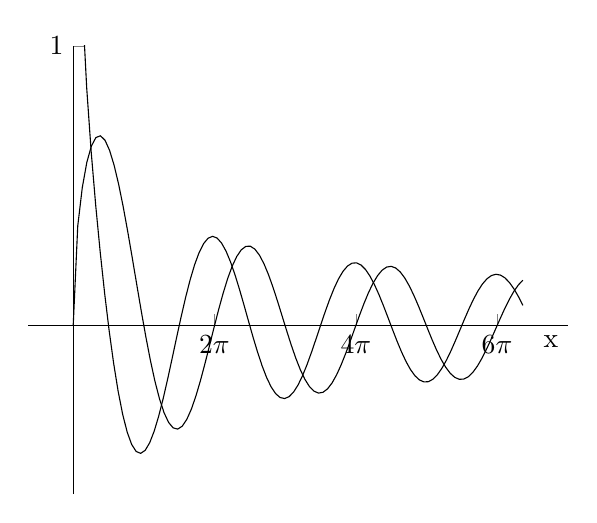
\begin{tikzpicture}
\begin{axis}[axis lines*=middle,xlabel=x,xlabel style={at={(current axis.right of origin)},anchor=north east},ytick={0,1},yticklabels={$0$,$1$},xtick={6.28,12.57,18.85},xticklabels={$2\pi$,$4\pi$,$6\pi$},ymax=1]
\addplot[domain=0:20,samples=100]{sqrt(2/(pi*x))*sin(180/pi*x)};
\addplot[domain=0.2:20,samples=100]{sqrt(2/(pi*x))*cos(180/pi*x)};
\end{axis}
\end{tikzpicture}
\caption{بیسل تفاعل \عددی{J_{\tfrac{1}{2}}(x)} اور \عددی{J_{-\tfrac{1}{2}}(x)}}
\label{شکل_بیسل_کسری_بیسل}
\end{figure}

مساوت \حوالہ{مساوات_بیسل_تعلق_الف} استعمال کرتے ہوئے
\begin{align*}
[\sqrt{x}J_{\tfrac{1}{2}}(x)]'=\sqrt{\frac{2}{\pi}}\cos x=\sqrt{x}J_{-\tfrac{1}{2}}(x)
\end{align*} 
لکھا جا سکتا ہے جس میں دائیں ہاتھ کے مساوات کو لیتے ہوئے \عددی{\sqrt{x}} سے تقسیم کرتے ہوئے مساوات \حوالہ{مساوات_بیسل_تعلق_کوسائن} کی دوسری مساوات ملتی ہے۔
\انتہا{مثال}
%=============================

\جزوحصہء{عمومی حل۔ خطی طور تابعیت}
بیسل مساوات \حوالہ{مساوات_بیسل_الف} کے عمومی حل کے لئے \عددی{J_v(x)} کے علاوہ خطی طور غیر تابع دوسرا حل بھی درکار ہے۔غیر عدد صحیح \عددی{\nu} کی صورت میں دوسرا حل  \عددی{r_2=-\nu} (اشاری مساوات \حوالہ{مساوات_بیسل_ت}) استعمال کرتے ہوئے حاصل ہو گا۔یوں دوسرا خطی طور غیر تابع حل مساوات \حوالہ{مساوات_بیسل_تسلسل_عمومی} میں \عددی{\nu} کی جگہ \عددی{-\nu} پر کرنے سے حاصل ہو گا۔
\begin{align}\label{مساوات_بیسل_تسلسل_عمومی_دوسرا}
J_{-\nu}(x)=x^{-\nu}\sum_{m=0}^{\infty}\frac{(-1)^m x^{2m}}{2^{2m-\nu}m!\Gamma(m-\nu+1)}
\end{align}
\عددی{\nu} غیر عدد صحیح ہونے کی صورت میں \عددی{J_{\nu}} اور \عددی{J_{-\nu}} خطی طور غیر تابع ہیں۔یوں غیر عدد صحیح \عددی{\nu} کی صورت میں \عددی{x \ne 0} پر  مساوات بیسل کا عمومی حل 
\begin{align}
y(x)=c_1J_{\nu}(x)+c_2J_{-\nu}(x)
\end{align}
ہو گا۔ 

\عددی{\nu} عدد صحیح ہونے کی صورت میں \عددی{J_n(x)} اور \عددی{J_{-n}(x)} کا تعلق
\begin{align}\label{مساوات_بیسل_عدد_صحیح_بیسل_تعلق}
J_{-n}(x)=(-1)^nJ_n(x) \quad \quad (n=1,2,\cdots)
\end{align}
ہے لہٰذا یہ خطی طور تابع ہیں اور ان سے عمومی حل نہیں لکھا جا سکتا ہے۔آئیں مساوات \حوالہ{مساوات_بیسل_عدد_صحیح_بیسل_تعلق} کو ثابت کریں۔

%==============================
\ابتدا{ثبوت}
مساوات \حوالہ{مساوات_بیسل_تسلسل_عمومی_دوسرا} میں \عددی{\nu} کی قیمت کو عدد صحیح کے قریب تر لانے سے گیما تفاعل کی قیمت (صفحہ \حوالہصفحہ{شکل_ضمیمہ_مفید_گیما_تفاعل} پر شکل \حوالہ{شکل_ضمیمہ_مفید_گیما_تفاعل}) لامتناہی کی طرف بڑھتی ہے۔یوں \عددی{\nu=n} کی صورت میں مساوات \حوالہ{مساوات_بیسل_تسلسل_عمومی_دوسرا} کے ابتدائی \عددی{n} ارکان کے عددی سر، گیما تفاعل کی قیمت لامتناہی ہونے کی بنا، صفر ہوں گے اور یوں تسلسل \عددی{m=n} سے شروع ہو گا۔مساوات \حوالہ{مساوات_بیسل_گیما_بطور_عدد_ضربیہ} کے تحت \عددی{\Gamma(m-n+1)=(m-n)!} ہے لہٰذا درج ذیل لکھا جائے گا
\begin{align*}
J_{-n}(x)=\sum_{m=n}^{\infty}\frac{(-1)^mx^{2m-n}}{2^{2m-n}m!(m-n)!}=\sum_{s=0}^{\infty}\frac{(-1)^{n+s}x^{2s+n}}{2^{2s+n} (n+s)!s!}\quad \quad (m=n+s)
\end{align*}
جو \عددی{(-1)^nJ_n(x)} ہے۔
\انتہا{ثبوت}
%==========================

اگلے حصے میں \عددی{\nu=n} کی صورت میں مساوات بیسل کا عمومی حل، بیسل تفاعل کی دوسری قسم \عددی{Y_{\nu}} کی مدد سے، حاصل کیا جائے گا۔
%==================

\حصہء{سوالات}

 %==================
\ابتدا{سوال}
ثابت کریں کہ \عددی{J_n(x)} تمام \عددی{x} کے لئے مرتکز ہے۔

جواب: \عددی{\abs{\tfrac{a_{m+1}}{a_m}}=\tfrac{2^{2m+n}m!(n+m)!}{2^{2m+2+n} (m+1)!(n+m+1)!}=\tfrac{1}{2^2(m+1)(n+m+1)}} ہے لہٰذا 
\عددی{\abs{\tfrac{a_{m+1}}{a_m}}_{m\to \infty}=0} اور یوں \عددی{R\to \infty} ہو گا۔
\انتہا{سوال}
%====================
سوال \حوالہ{سوال_بیسل_صورت_الف} تا سوال \حوالہ{سوال_بیسل_صورت_ب} کے عمومی حل، جہاں ممکن ہو،  \عددی{J_{\nu}} اور \عددی{J_{-\nu}} استعمال کرتے ہوئے لکھیں۔جہاں اضافی معلومات دی گئی ہوں، وہاں اس کو استعمال کرتے ہوئے بیسل مساوات کی صورت حاصل کریں۔

%============
\ابتدا{سوال}\شناخت{سوال_بیسل_صورت_الف}\quad
$x^2y''+xy'(x^2-\frac{4}{9})y=0$\\
جواب:چونکہ \عددی{\nu=\tfrac{2}{3}} ہے جو غیر عدد صحیح ہے لہٰذا عمومی حل \عددی{y=c_1J_{\tfrac{2}{3}}+c_2J_{-\tfrac{2}{3}}} ہے۔
\انتہا{سوال}
%=================
\ابتدا{سوال}\quad
$xy''+y'+\frac{1}{4}y\quad \quad (z=\sqrt{x})$\\
جواب:\عددی{y=c_1J_0(\sqrt{x})}
\انتہا{سوال}
%=================
\ابتدا{سوال}\quad
$xy''+y'+\frac{x}{4}y=0\quad \quad (z=\frac{x}{2})$\\
جواب:\عددی{y=c_1J_0(\tfrac{x}{2})}
\انتہا{سوال}
%===================
\ابتدا{سوال}\quad
$x^2y''+xy'(\frac{x^2}{9}-\frac{1}{9})y=0\quad \quad (z=\frac{x}{3})$\\
جواب:\عددی{y=c_1J_{\tfrac{1}{3}}(\tfrac{x}{3})+c_2J_{-\tfrac{1}{3}}(\tfrac{x}{3})}
\انتہا{سوال}
%====================
\ابتدا{سوال}\quad
$y''+(e^{2x}-16)y=0,\quad \quad (z=e^x)$\\
جواب:\عددی{y=c_1J_4(e^x)}
\انتہا{سوال}
%=================
\ابتدا{سوال}\quad
$x^2y''+xy'(\lambda^2 x^2-\nu^2)y=0,\quad \quad (z=\lambda x)$\\
جواب:\عددی{y=c_1 J_{\nu}(\lambda x)+c_2J_{-\nu}(\lambda x)} جہاں \عددی{\nu \ne 0, \mp1, \mp2, \cdots}
\انتہا{سوال}
%=================
\ابتدا{سوال}\quad
$x^2y''+xy'+(9x^2-1)y=0,\quad \quad (z=3x)$\\
جواب:\عددی{y=c_1J_1(3x)}
\انتہا{سوال}
%======================
\ابتدا{سوال}\quad
$(x-\frac{1}{2})^2y''+(x-\frac{1}{2})y'+4x(x-1)y=0\quad \quad(z=2x-1)$\\
جواب:\عددی{y=c_1J_1(2x-1)}
\انتہا{سوال}
%==================
\ابتدا{سوال}\quad
$xy''+(2\nu+1)y'+xy=0,\quad \quad y=x^{-\nu}u$\\
جواب:\عددی{y=x^{-\nu}(c_1J_{\nu}(x)+c_2J_{-\nu}(x))} جہاں \عددی{\nu \ne 0,\mp1,\mp2,\cdots}
\انتہا{سوال}
%====================
\ابتدا{سوال}\شناخت{سوال_بیسل_صورت_ب}\quad
$x^2y''+\frac{1}{4}(x+\frac{3}{4})y=0,\quad \quad y=u\sqrt{x}, \quad z=\sqrt{x}$\\
جواب:\عددی{y=c_1\sqrt{x}J_{\tfrac{1}{2}}(\sqrt{x})+c_2\sqrt{x}J_{-\tfrac{1}{2}}(\sqrt{x})}
\انتہا{سوال}
%====================
\ابتدا{سوال}
مساوات \حوالہ{مساوات_بیسل_تعلق_پ} اور مساوات \حوالہ{مساوات_بیسل_تعلق_کوسائن} سے درج ذیل ثابت کریں۔
\begin{align}
J_{\tfrac{3}{2}}(x)=\sqrt{\frac{2}{\pi x}} \left(\frac{\sin x}{x}-\cos x\right), \quad  J_{-\tfrac{3}{2}}(x)=-\sqrt{\frac{2}{\pi x}}\left(\frac{\cos x}{x}+\sin x \right)
\end{align}
\انتہا{سوال}
%======================
\ابتدا{سوال}
کیا آپ مساوات \حوالہ{مساوات_بیسل_تعلق_پ} اور مساوات \حوالہ{مساوات_بیسل_تعلق_کوسائن} سے  اخذ کر سکتے ہیں کہ
 \عددی{\nu=\mp \tfrac{1}{2},\mp\tfrac{3}{2},\mp\tfrac{5}{2},\cdots} کی صورت میں \عددی{J_{\nu}(x)} بنیادی تفاعل ہیں۔

جواب:جی ہاں۔
\انتہا{سوال}
%=====================

%================
\ابتدا{سوال}\quad باہم پیچاں صفر\\
مساوات \حوالہ{مساوات_بیسل_تعلق_الف}، مساوات \حوالہ{مساوات_بیسل_تعلق_ب} اور \اصطلاح{مسئلہ رول}\فرہنگ{مسئلہ!رول}\فرہنگ{رول مسئلہ}\حاشیہب{Rolle's theorem}\فرہنگ{theorem!Rolle's} استعمال کرتے ہوئے ثابت کریں کہ \عددی{J_n(x)} کے کسی بھی دو متواتر صفروں کے مابین \عددی{J_{n+1}(x)} کا ایک صفر پایا جاتا ہے۔ 

جواب:مسئلہ رول کہتا ہے کہ کسی بھی حقیقی قابل تفرق تفاعل کے دو متواتر برابر قیمت نقطوں کے مابین کم از کم ایک ایسا نقطہ (نقطہ فاصل) پایا جاتا ہے جس پر تفاعل کا تفرق صفر کے برابر ہو گا۔ اگر \عددی{J_n(x)} کے دو متواتر صفر \عددی{x_1} اور \عددی{x_2} پر پائے جاتے ہوں تب ہم \عددی{x_1^{-n}J_n(x_1)=x_2^{-n}J_n(x_2)=0} لکھ سکتے ہیں۔یوں مسئلہ رول کے تحت \عددی{x_1} اور \عددی{x_2} کے مابین کسی نقطے پر تفاعل \عددی{x^{-n}J_n(x)} کا تفرق صفر \عددی{[x^{-n}J_n(x)]'=0} ہو گا جو مساوات \حوالہ{مساوات_بیسل_تعلق_ب} کے استعمال سے ایسے نقطے پر \عددی{x^{-n}J_{n+1}(x)=0} یعنی \عددی{J_{n+1}(x)=0} دیتا ہے۔اسی طرح اگر \عددی{J_{n+1}(x)} کے دو متواتر صفر \عددی{x_3} اور \عددی{x_4} پر پائے جاتے ہوں تب \عددی{J_{n+1}(x_3)=J_{n+1}(x_4)=0} اور \عددی{x_3^{n+1}J_{n+1}(x_3)=x_4^{n+1}J_{n+1}(x_4)=0} لکھا جا سکتا ہے۔یوں مسئلہ رول کے تحت \عددی{x_3} اور \عددی{x_4} کے مابین کسی نقطے پر \عددی{[x^{n+1}J_{n+1}(x)]'=0} ہو گا جس سے مساوات \حوالہ{مساوات_بیسل_تعلق_الف} کے تحت ایسے نقطے پر \عددی{x^{n+1}J_n(x)=0} یعنی \عددی{J_n(x)=0} حاصل ہوتا ہے۔ یوں  ثابت ہوا کہ \عددی{J_{n+1}} کے دو متواتر صفر \عددی{x_3} اور \عددی{x_4} کے مابین \عددی{J_n(x)} کا صفر پایا جاتا ہے جبکہ \عددی{J_n(x)} کے دو متواتر صفر \عددی{x_1} اور \عددی{x_2} کے مابین \عددی{J_{n+1}(x)} کا صفر پایا جاتا ہے۔
\انتہا{سوال}
%=================
\ابتدا{سوال}\quad تفرقی مساوات سے ایک درجی تفرق کا اخراج\\
 درج ذیل تفرقی مساوات میں \عددی{y(x)=u(x)v(x)} پر کرتے ہوئے ایسا \عددی{v(x)} دریافت کریں کہ حاصل تفرقی مساوات میں پہلے درجے کا تفرق نہ پایا جاتا ہو۔حاصل تفرقی مساوات بھی حاصل کریں۔
\begin{align*}
y''+p(x)y'+q(x)y=0
\end{align*}
جوابات:\عددی{v=e^{-\tfrac{1}{2}\int p(x)\dif x}} اور مساوات \عددی{u''+[q-\tfrac{1}{4}p^2-\tfrac{1}{2}p']u=0} میں \عددی{u'} نہیں پایا جاتا ہے۔

\انتہا{سوال}
%=====================
\ابتدا{سوال}
گزشتہ سوال میں تفرقی مساوات سے ایک درجی تفرق کا اخراج کیا گیا۔ثابت کریں کہ مساوات بیسل \حوالہ{مساوات_بیسل_الف} سے ایک درجی تفرق کا اخراج \عددی{y=\tfrac{u}{\sqrt{x}}} پر کرتے ہوئے ہو گا جس سے درج ذیل تفرقی مساوات حاصل ہو گی۔
\begin{align}\label{مساوات_بیسل_سادہ_صورت}
x^2u''+(x^2+\tfrac{1}{4}-\nu^2)u=0
\end{align}
\انتہا{سوال}
%====================
\ابتدا{سوال}
مساوات \حوالہ{مساوات_بیسل_سادہ_صورت} کا عمومی حل \عددی{\nu=\tfrac{1}{2}} کے لئے حاصل کریں۔

جواب: \عددی{u=A\cos x+B\sin x} ہے لہٰذا \عددی{y=\tfrac{u}{\sqrt{x}}=\tfrac{1}{\sqrt{x}}(A\cos x+B\sin x)} ہو گا۔
\انتہا{سوال}
%===================
سوال \حوالہ{سوال_بیسل_تفرق_تکمل_الف} تا سوال \حوالہ{سوال_بیسل_تفرق_تکمل_ب}  مساوات \حوالہ{مساوات_بیسل_تعلق_الف} اور مساوات \حوالہ{مساوات_بیسل_تعلق_ب} کی مدد سے حل ہوں گے۔

%===============
\ابتدا{سوال}\شناخت{سوال_بیسل_تفرق_تکمل_الف}\quad ثابت کریں 
$J'_0(x)=-J_1(x),\quad J'_1(x)=J_0(x)-\frac{J_1(x)}{x},\quad J'_2(x)=\frac{1}{2}[J_1(x)-J_3(x)]$\\
\انتہا{سوال}
%=================
\ابتدا{سوال}
بیسل مساوات \حوالہ{مساوات_بیسل_الف} کو مساوات \حوالہ{مساوات_بیسل_تعلق_الف} اور مساوات \حوالہ{مساوات_بیسل_تعلق_ب} سے حاصل کریں۔
\انتہا{سوال}
%=====================
\ابتدا{سوال}
درج ذیل ثابت کریں
\begin{align*} 
\int x^{\nu} J_{\nu-1}(x)\dif x&=x^{\nu}J_{\nu}(x)+c\\
\int x^{-\nu}J_{\nu+1}\dif x&=-x^{-\nu}J_{\nu}(x)+c\\
\int J_{\nu+1}(x)\dif x&=\int J_{\nu-1}(x)\dif x-2J_{\nu}(x)
\end{align*}
\انتہا{سوال}
%======================
\ابتدا{سوال}\quad
$\int J_3(x)\dif x$\\
جواب:مساوات \حوالہ{مساوات_بیسل_تعلق_ت} میں \عددی{\nu=2} پر کر کے تکمل \عددی{\int J_3\dif x=\int  J_1\dif x-2J_2} ہو گا اور مساوات \حوالہ{مساوات_بیسل_تعلق_ب} میں \عددی{\nu=0} پر کرتے ہوئے تکمل \عددی{\int J_1\dif x=-J_0} دیتا ہے لہٰذا \عددی{\int J_3\dif x=-J_0-2J_2+c} 
\انتہا{سوال}
%=====================
\ابتدا{سوال} تکمل بالحصص استعمال کرتے  ہوئے حل کریں۔\quad 
$\int x^3J_0(x)\dif x$\\
جواب:
$\int x^3J_0\dif x=\int x^2(xJ_0)\dif x=x^2(xJ_1)-2\int x^2J_1\dif x=x^3J_1-2x^2J_2+c$
\انتہا{سوال}
%=======================
\ابتدا{سوال} \شناخت{سوال_بیسل_تفرق_تکمل_ب} تکمل بالحصص سے حل کریں۔\quad 
$\int x^2J_0\dif x$\\
جواب:\عددی{\int x^2J_0\dif x=x^2J_1+xJ_0-\int J_0\dif x}، جہاں \عددی{\int J_0\dif x} کسی بنیادی تفاعل کی صورت میں نہیں لکھا جا سکتا ہے بلکہ اس کی قیمت  جدول کی مدد سے لکھی جاتی ہے۔

\انتہا{سوال}
%===================

\حصہ{بیسل تفاعل کی دوسری قسم۔ عمومی حل}
بیسل مساوات \حوالہ{مساوات_بیسل_الف} کا کسی بھی \عددی{\nu} کے لئے عمومی حل حاصل کرنے کی خاطر \اصطلاح{بیسل تفاعل کی دوسری قسم}\فرہنگ{بیسل تفاعل!دوسری قسم}\حاشیہب{Bessel function of the second kind}\فرہنگ{Bessel!second kind function} \عددی{Y_{\nu}(x)} حاصل کرتے ہیں۔شروع \عددی{\nu=n=0} سے کرتے ہیں۔  

\عددی{n=0} کی صورت میں مساوات بیسل کو \عددی{x} سے تقسیم کرتے ہوئے
\begin{align}\label{مساوات_بیسل_دوہرا_صفر_الف}
xy''+y'+xy=0
\end{align}
لکھا جا سکتا ہے اور اشاری مساوات \حوالہ{مساوات_طاقتی_اشاری_مساوات} سے دوہرا جذر \عددی{r=0} ملتا ہے  جو صفحہ \حوالہصفحہ{مسئلہ_طاقتی_فروبنیوس_اساس} پر مسئلہ فروبنیوس میں بتلائی گئی دوسری صورت کو ظاہر کرتی ہے۔یوں مساوات \حوالہ{مساوات_بیسل_دوہرا_صفر_الف} کا ایک حل \عددی{J_0(x)} ہو گا جبکہ اس کا دوسرا حل مساوات \حوالہ{مساوات_طاقتی_فروبنیوس_حل_ت} میں \عددی{r=0} پر کرتے ہوئے  
\begin{align}\label{مساوات_بیسل_دوہرا_صفر_ب}
y_2(x)=J_0(x)\ln x+\sum_{m=1}^{\infty}A_m x^m 
\end{align}
لکھا جائے گا۔مساوات \حوالہ{مساوات_بیسل_دوہرا_صفر_ب} اور اس کے تفرقات
\begin{align*}
y_2'&=J_0' \ln x+\frac{J_0}{x}+\sum_{m=1}^{\infty}mA_mx^{m-1}\\
y_2''&=J_0''\ln x+\frac{2J_0'}{x}-\frac{J_0}{x}+\sum_{m=1}^{\infty} m(m-1)A_m x^{m-2}
\end{align*}
کو مساوات \حوالہ{مساوات_بیسل_دوہرا_صفر_الف} میں پر کرتے ہیں (اگرچہ آخری مجموعے کا پہلا رکن \عددی{m=2} لکھنا چاہیے، البتہ \عددی{m=1} پر دیا گیا مجموعہ صفر دیتا ہے لہٰذا مجموعے کا پہلا رکن \عددی{m=1} لکھنا ممکن ہے)۔اب چونکہ \عددی{J_0} تفرقی مساوات کا حل ہے لہٰذا  تین لوگارتھمی ارکان کا مجموعہ \عددی{(xJ_0''+J_0'+xJ_0)\ln x} صفر کے برابر ہو گا اور یوں بقایا درج ذیل ہو گا۔
\begin{align*}
2J_0'+\sum_{m=1}^{\infty}m(m-1)A_mx^{m-1}+\sum_{m=1}^{\infty}mA_mx^{m-1}+\sum_{m=1}^{\infty}A_mx^{m+1}=0
\end{align*}
اس میں پہلے اور دوسرے  مجموعوں کو جمع کرتے ہوئے \عددی{\sum m^2A_mx^{m-1}} لکھا کر جبکہ \عددی{J_0'} کی طاقتی تسلسل کو مساوات \حوالہ{مساوات_بیسل_د} کا جزو در جزو تفرق لیتے اور \عددی{\tfrac{m!}{m}=(m-1)!} استعمال کرتے ہوئے
\begin{align*}
J'_0(x)=\sum_{m=1}^{\infty}\frac{(-1)^m2mx^{2m-1}}{2^{2m}(m!)^2}=\sum_{m=1}^{\infty}\frac{(-1)^mx^{2m-1}}{2^{2m-1}m!(m-1)!}
\end{align*} 
لکھ کر درج ذیل حاصل ہوتا ہے۔
\begin{align}\label{مساوات_بیسل_دوہرا_صفر_پ}
\sum_{m=1}^{\infty}\frac{(-1)^mx^{2m-1}}{2^{2m-2}m!(m-1)!}+\sum_{m=1}^{\infty} m^2A_mx^{m-1}+\sum_{m=1}^{\infty}A_mx^{m+1}=0
\end{align}
اس مساوات میں \عددی{x^0} کمتر طاقت، جو صرف دوسرے مجموعے میں پایا جاتا ہے، کے عددی سر کو صفر کے برابر پر کرتے ہوئے \عددی{A_1=0} ملتا ہے۔اب \عددی{x^{2s}} کے عددی سروں، جو پہلے تسلسل میں نہیں پایا جاتا، کے مجموعے کو صفر کے برابر لکھتے ہیں۔
\begin{align*}
(2s+1)^2A_{2s+1}+A_{2s-1}=0,\quad \quad (s=1,2,\cdots)
\end{align*}
اب چونکہ \عددی{A_1=0} ہے لہٰذا \عددی{A_3=0}، \عددی{A_5=0}، \نقطے ہوں گے۔ 

\عددی{x^{2s+1}} کے عددی سروں کے مجموعے کو صفر کے برابر پر کرتے ہوئے \عددی{s=0} کے لئے
\begin{align*}
-1+4A_2=0, \quad \implies \quad A_2=\frac{1}{4}
\end{align*}
جبکہ بقایا \عددی{s} پر
\begin{align*}
\frac{(-1)^{s+1}}{2^{2s}(s+1)!s!}+(2s+2)^2A_{2s+2}+A_{2s}=0,\quad (s=1,2,\cdots)
\end{align*}
لکھا جائے گا۔اس سے \عددی{s=1} کے لئے
\begin{align*}
\frac{1}{8}+16A_4+A_2=0\quad \implies \quad A_4=-\frac{3}{128}
\end{align*}
حاصل ہوتا ہے جبکہ عمومی طور پر
\begin{align}\label{مساوات_بیسل_دوہرا_صفر_ت}
A_{2m}=\frac{(-1)^{m-1}}{2^{2m}(m!)^2}\left(1+\frac{1}{2}+\frac{1}{3}+\cdots+\frac{1}{m}\right), \quad \quad (m=1,2,\cdots)
\end{align}
ملتا ہے۔قوسین میں بند قیمت کو \عددی{h_m} لکھ کر،
\begin{align}\label{مساوات_بیسل_دوہرا_صفر_ٹ}
h_m=1+\frac{1}{2}+\frac{1}{3}+\cdots+\frac{1}{m}
\end{align}
مساوات \حوالہ{مساوات_بیسل_دوہرا_صفر_ت} اور \عددی{A_1=A_3=\cdots=0} کو مساوات \حوالہ{مساوات_بیسل_دوہرا_صفر_ب} میں پر کرتے ہوئے جواب حاصل کرتے ہیں۔
\begin{gather}
\begin{aligned}
y_2(x)&=J_0(x)\ln x+\sum_{m=1}^{\infty}\frac{(-1)^{m-1}h_m}{2^{2m}(m!)^2}x^{2m}\\
&=J_0(x)\ln x+\frac{1}{4}x^2-\frac{3}{128}x^4+\frac{11}{\num{13824}}x^6-+\cdots
\end{aligned}
\end{gather}
چونکہ \عددی{J_0} اور \عددی{y_2} خطی طور غیر تابع ہیں لہٰذا یہ مساوات بیسل \حوالہ{مساوات_بیسل_الف} کی حل کی اساس ہیں۔ہم \عددی{J_0} اور \عددی{y_2} سے کوئی بھی مخصوص حل، \عددی{a(y_2+bJ_0)} جہاں \عددی{a(\ne 0)} اور \عددی{b} مستقل ہیں، لکھتے ہوئے اساس کی مختلف صورتیں حاصل کر سکتے ہیں۔روایتی طور پر \عددی{a=\tfrac{2}{\pi}} اور \عددی{b=\gamma-\ln 2} چننے جاتے ہیں جہاں \عددی{\gamma=\num{0.57721566490}\cdots} \اصطلاح{مستقل یولر}\فرہنگ{یولر!مستقل}\حاشیہب{Euler constant}\فرہنگ{Euler!constant} کہلاتا ہے جس کی تعریف درج ذیل ہے جہاں \عددی{s} کی قیمت لامتناہی کو چھونے کی کوشش کرتی ہے۔
\begin{align}
\gamma=1+\frac{1}{2}+\cdots+\frac{1}{s}-\ln s
\end{align}
اس طرح لکھا گیا دوسرا حل \اصطلاح{درجہ صفر بیسل تفاعل کی دوسری قسم}\فرہنگ{بیسل تفاعل!درجہ صفر، دوسری قسم}\حاشیہب{Bessel function of the second kind of order zero}\فرہنگ{Bessel function!second kind} (شکل \حوالہ{شکل_بیسل_نیومن_درجہ_صفر}) یا \اصطلاح{درجہ صفر نیومن تفاعل}\فرہنگ{نیومن تفاعل!درجہ صفر}\فرہنگ{تفاعل!نیومن، درجہ صفر}\حاشیہب{Neumann's function of order zero}\فرہنگ{Neumann's function} کہلاتا\حاشیہد{کارل نیومن [1832-1925] جرمنی کے ریاضی دان اور ماہر طبیعیات۔} اور \عددی{Y_0(x)} سے ظاہر کیا جاتا ہے۔یوں
\begin{align}\label{مساوات_بیسل_نیومن_درجہ_صفر}
Y_0(x)=\frac{2}{\pi}\left[J_0(x) \left(\ln \frac{x}{2}+\gamma\right)+\sum_{m=1}^{\infty} \frac{(-1)^{m-1} h_m}{2^{2m}(m!)^2}x^{2m}\right]
\end{align}
لکھا جائے گا جہاں \عددی{h_m} کی قیمت مساوات \حوالہ{مساوات_بیسل_دوہرا_صفر_ٹ}  دیتی ہے۔
\begin{figure}
\centering
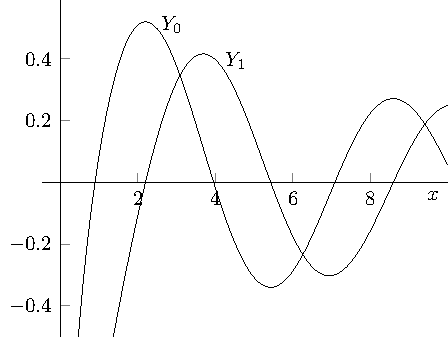
\includegraphics{figOctaveNeumannFunction}
\caption{بیسل تفاعل کے دوسرے اقسام۔}
\label{شکل_بیسل_نیومن_درجہ_صفر}
\end{figure}
جیسا شکل \حوالہ{شکل_بیسل_نیومن_درجہ_صفر} میں دکھایا گیا ہے کم قیمت کی مثبت \عددی{x} پر \عددی{Y_0} کی صورت \عددی{\ln x} کی طرح ہے اور \عددی{x\to \infty} پر \عددی{Y_0(x) \to \infty} ہو گا۔

\عددی{\nu=n=1,2,\cdots} کے لئے بھی بالکل اسی طرح، مساوات \حوالہ{مساوات_طاقتی_فروبنیوس_حل_ث} سے شروع کرتے ہوئے  دوسرا حل حاصل کیا جاتا ہے۔ان میں بھی لوگارتھمی جزو پایا جاتا ہے۔

دوسرے حل کا دارومدار اس حقیقت پر ہے کہ آیا \عددی{\nu} کا درجہ عدد صحیح ہے یا نہیں۔اس پیچیدگی  سے چھٹکارا حاصل کرنے کی خاطر دوسرے حل کو درج ذیل بیان کیا جاتا ہے جو تمام \عددی{\nu} کے لئے قابل استعمال ہے۔
\begin{gather}
\begin{aligned}\label{مساوات_بیسل_نیومن_عمومی_حل_الف}
Y_{\nu}(x)&=\frac{1}{\sin \nu \pi} [J_{\nu}(x)\cos \nu x-J_{-\nu}(x)] \quad \quad \text{(الف)}\\
Y_n(x)&=\lim_{\nu \to n} Y_{\nu}(x)\quad \quad \text{(ب)}
\end{aligned}
\end{gather}
درج بالا تفاعل کو \اصطلاح{درجہ \عددی{\nu} بیسل تفاعل کی دوسری قسم}\فرہنگ{بیسل تفاعل!دوسری قسم، درجہ \عددی{\nu}}\حاشیہب{Bessel function of the second kind of order $\nu$}\فرہنگ{Bessel function!second kind, order $\nu$} یا \اصطلاح{درجہ \عددی{\nu} نیومن تفاعل} کہتے ہیں۔ 

آئیں اب ثابت کریں کہ \عددی{J_{\nu}} اور \عددی{Y_{\nu}} تمام \عددی{\nu} اور تمام \عددی{x(>0)} کے لئے خطی طور غیر تابع ہیں۔

غیر عددی صحیح درجہ \عددی{\nu} کے لئے چونکہ \عددی{J_{\nu}(x)} اور \عددی{J_{-\nu}(x)} بیسل مساوات کے حل ہیں لہٰذا   \عددی{Y_{\nu}(x)} بھی بیسل مساوات کا حل ہے۔اب چونکہ ایسی \عددی{\nu} کے لئے \عددی{J_{\nu}(x)} اور \عددی{J_{-\nu}(x)} خطی طور غیر تابع ہیں اور \عددی{Y_{\nu}(x)} میں \عددی{J_{-\nu}(x)} پایا جاتا ہے لہٰذا \عددی{J_{\nu}(x)} اور \عددی{Y_{\nu}(x)} خطی طور غیر تابع ہوں گے۔مزید یہ کہ مساوات \حوالہ{مساوات_بیسل_نیومن_عمومی_حل_الف}-ب کو ثابت (صفحہ \حوالہصفحہ{حوالہ_بیرونی_مواد} پر حوالہ \cite{حوالہ_کریزگ_ب_اٹھارہ} میں ثبوت پیش کیا گیا ہے۔) کیا جا سکتا ہے لہٰذا عدد صحیح درجہ کے لئے \عددی{Y_n(x)} بیسل مساوات کا حل ہے۔آپ دیکھیں گے کہ \عددی{Y_n(x)} کی تسلسل میں لوگارتھمی جزو پایا جاتا ہے لہٰذا \عددی{J_n(x)} اور \عددی{Y_n(x)} خطی طور غیر تابع ہوں گے۔\عددی{Y_n(x)} کی تسلسل لکھنے کی خاطر \عددی{J_{\nu}(x)} کی تسلسل \حوالہ{مساوات_بیسل_تسلسل_عمومی} اور \عددی{J_{-\nu}(x)} کی تسلسل \حوالہ{مساوات_بیسل_تسلسل_عمومی_دوسرا} کو مساوات \حوالہ{مساوات_بیسل_نیومن_عمومی_حل_الف}-الف میں پر کرتے ہوئے \عددی{\nu \to n} کرتے ہیں (تفصیل صفحہ \حوالہصفحہ{حوالہ_بیرونی_مواد} پر \cite{حوالہ_کریزگ_ب_اٹھارہ} سے دیکھی جا سکتی ہے۔)
\begin{multline}\label{مساوات_بیسل_نیومن_عدد_صحیح_الف}
Y_n(x)=\frac{2}{\pi}J_n(x)\left(\ln \frac{x}{2}+\gamma\right)+\frac{x^n}{\pi}\sum_{m=0}^{\infty} \frac{(-1)^{m-1}(h_m+h_{m+n})}{2^{2m+n}m!(m+n)!}x^{2m}\\
-\frac{x^{-n}}{\pi}\sum_{m=0}^{n-1}\frac{(n-m-1)!}{2^{2m-n}m!}x^{2m}
\end{multline}
لکھا جا سکتا ہے جہاں \عددی{x>0} اور  \عددی{n=0,1,\cdots} جبکہ
\begin{align*}
h_0=0,\quad h_s=1+\frac{1}{2}+\frac{1}{3}+\cdots+\frac{1}{s} \quad \quad (s=1,2,\cdots)
\end{align*}
ہیں اور \عددی{n=0} کی صورت میں مساوات \حوالہ{مساوات_بیسل_نیومن_عدد_صحیح_الف} میں آخری مجموعے کی جگہ صفر لکھا جاتا ہے۔ درجہ صفر \عددی{n=0} پر  مساوات \حوالہ{مساوات_بیسل_نیومن_عدد_صحیح_الف} عین مساوات \حوالہ{مساوات_بیسل_نیومن_درجہ_صفر} کی صورت اختیار کرتی ہے۔اس کے علاوہ درج ذیل ثابت کیا جا سکتا ہے۔
\begin{align}
Y_{-n}(x)=(-1)^nY_n(x)
\end{align}
ان نتائج کو درج ذیل مسئلے میں پیش کرتے ہیں۔

%=======================
\ابتدا{مسئلہ} مساوات بیسل کا عمومی حل\\
تمام \عددی{\nu} کے لئے مساوات بیسل کا عمومی حل درج ذیل ہے۔
\begin{align}
y(x)=c_1J_{\nu}(x)+c_2Y_{\nu}(x)
\end{align}
\انتہا{مسئلہ}
%========================

بعض اوقات حقیقی \عددی{x} کے لئے مساوات بیسل کے مخلوط حل درکار ہوتے ہیں۔ایسی صورت میں درج ذیل خطی طور غیر تابع مخلوط حل  استعمال کیے جاتے ہیں جنہیں \اصطلاح{درجہ \عددی{\nu} بیسل تفاعل کی تیسری قسم}\فرہنگ{بیسل تفاعل!تیسری قسم}\حاشیہب{Bessel function of the third kind of order $\nu$}\فرہنگ{Bessel function!third kind} یا درجہ \عددی{\nu} پہلی اور دوسری \اصطلاح{ہینکل تفاعل}\فرہنگ{ہینکل تفاعل}\فرہنگ{تفاعل!ہینکل}\حاشیہب{Hankel functions}\فرہنگ{Hankel functions} کہا\حاشیہد{ہرمن ہینکل [1839-1873] جرمنی کے ریاضی دان۔} جاتا ہے۔
\begin{gather}
\begin{aligned}\label{مساوات_بیسل_ہینکل}
H_{\nu}^1(x)&=J_{\nu}(x)+iY_{\nu}(x)\\
H_{\nu}^2(x)&=J_{\nu}(x)-iY_{\nu}(x)
\end{aligned}
\end{gather}
%========================

\حصہء{سوالات}
سوال \حوالہ{سوال_بیسل_عمومی_حل_نیومن_الف} تا سوال \حوالہ{سوال_بیسل_عمومی_حل_نیومن_ب} کا عمومی حل \عددی{J_{\nu}} اور \عددی{Y_{\nu}} کی صورت میں حاصل کریں۔بتلائیں کہ کن سوالات میں \عددی{Y_{\nu}} کی جگہ \عددی{J_{-\nu}} استعمال کرنا ممکن ہے۔دی گئی اضافی معلومات استعمال کریں۔

%===============
\ابتدا{سوال}\شناخت{سوال_بیسل_عمومی_حل_نیومن_الف}\quad
$x^2y''+xy'+(x^2-25)y=0$\\
جواب:\عددی{y=c_1J_{5}(x)+c_2Y_{5}(x)}؛ چونکہ \عددی{\nu} عدد صحیح ہے لہٰذا \عددی{J_{-5}(x)} قابل استعمال نہیں ہے۔
\انتہا{سوال}
%=====================
\ابتدا{سوال}\quad
$x^2y''+xy'+(x^2-3)$\\
جواب:\عددی{y=c_1J_{\sqrt{3}}+c_2Y_{\sqrt{3}}(x)}؛ چونکہ \عددی{\nu} عدد صحیح نہیں ہے لہٰذا \عددی{J_{-\sqrt{3}}(x)} قابل استعمال ہے۔
\انتہا{سوال}
%===================
\ابتدا{سوال}\quad
$9x^2y''+9xy'+(z^{\tfrac{2}{3}}-\tfrac{9}{4})y=0, \quad \quad x=z^3$\\
جواب:\عددی{y=c_1J_{\tfrac{3}{2}}(x^{\tfrac{1}{3}})+c_2Y_{\tfrac{3}{2}}(x^{\tfrac{1}{3}})}
\انتہا{سوال}
%===================
\ابتدا{سوال}\quad
$x^2y''+xy'+(4x^4-\tfrac{16}{9})y=0,\quad \quad z=x^2$\\
جواب:\عددی{y=c_1J_{\tfrac{2}{3}}(x^2)+c_2Y_{\tfrac{2}{3}}(x^2)}
\انتہا{سوال}
%====================
\ابتدا{سوال}\quad
$9x^2y''+9xy'+(4x^{\tfrac{4}{3}}-25)y=0,\quad \quad z=x^{\tfrac{2}{3}}$\\
جواب:
$y=c_1J_{\tfrac{5}{2}}(x^{\tfrac{2}{3}})+c_2Y_{\tfrac{5}{2}}(x^{\tfrac{2}{3}})$
\انتہا{سوال}
%=================
\ابتدا{سوال}\quad
$y''+k^2x^2y=0,\quad \quad (y=u\sqrt{x},\quad z=\tfrac{kx^2}{2})$\\
جواب:\عددی{y=\sqrt{x}[c_1J_{\tfrac{1}{4}}(\tfrac{kx^2}{2})+c_2Y_{\tfrac{1}{4}}(\tfrac{kx^2}{2})]}
\انتہا{سوال}
%=================
\ابتدا{سوال}\quad
$xy''-5y'+xy=0,\quad \quad y=x^3u$\\
جواب:\عددی{y=x^3[c_1J_3(x)+c_2Y_3(x)]}
\انتہا{سوال}
%====================
\ابتدا{سوال}\quad
$xy''-y'+xy=0,\quad \quad y=xu$\\
جواب:\عددی{y=x[c_1J_1(x)+c_2Y_1(x)]}
\انتہا{سوال}
%=================
\ابتدا{سوال}\شناخت{سوال_بیسل_عمومی_حل_نیومن_ب}\quad
$xy''+5y'+xy=0,\quad \quad y=\tfrac{u}{x^2}$\\
جواب:\عددی{y=\tfrac{1}{x^2}[c_1J_2(x)+c_2Y_2(x)]}
\انتہا{سوال}
%===================
\ابتدا{سوال}\quad ترمیم شدہ درجہ \عددی{\nu} بیسل تفاعل کی پہلی قسم\\
ترمیم شدہ درجہ \عددی{\nu} بیسل تفاعل کی پہلی قسم کی تعریف \عددی{I_{\nu}(x)=i^{-\nu}J_{\nu}(ix)} ہے جہاں \عددی{i=\sqrt{-1}} ہے۔ثابت کریں  کہ \عددی{I_{\nu}(x)} درج ذیل تفرقی مساوات پر پورا اترتا ہے۔
\begin{align}\label{مساوت_بیسل_ترمیم_شدہ}
x^2y''+xy'-(x^2+\nu^2)y=0
\end{align}
جواب:\عددی{I_{\nu}(x)} کو دیے گئے مساوات میں پر کرتے ہوئے \عددی{0=0} حاصل کریں۔یہی ثبوت ہے۔
\انتہا{سوال}
%======================
\ابتدا{سوال}\quad ترمیم شدہ بیسل تفاعل\\
\عددی{I_{\nu}(x)} کی درج ذیل صورت حاصل کریں۔
\begin{align}
I_{\nu}(x)=\sum_{m=0}^{\infty}\frac{x^{2m+\nu}}{2^{2m+\nu}m!\Gamma(m+\nu+1)}
\end{align}
\انتہا{سوال}
%=======================
\ابتدا{سوال}\quad \عددی{I_{\nu}(x)} حقیقی ہے\\
ثابت کریں کہ حقیقی \عددی{x} اور حقیقی \عددی{\nu} کے لئے \عددی{I_{\nu}(x)} حقیقی ہے۔ثابت کریں کہ \عددی{x \ne 0} ہوتے ہوئے \عددی{I_{\nu}(x) \ne 0} ہو گا۔ ثابت کریں کہ \عددی{I_{-n}(x)=I_n(x)} کے برابر ہے جہاں \عددی{n} عدد صحیح ہے۔
\انتہا{سوال}
%====================
\ابتدا{سوال}\quad ترمیم شدہ بیسل تفاعل\\
ثابت کریں کہ تفاعل \عددی{K_{\nu}(x)}، جسے ترمیم شدہ بیسل تفاعل کی تیسری (بعض اوقات دوسری) قسم کہتے ہیں،
\begin{align}
K_{\nu}(x)=\frac{\pi}{2\sin \nu\pi}[I_{-\nu}(x)-I_{\nu}(x)]
\end{align}
تفرقی مساوات \حوالہ{مساوت_بیسل_ترمیم_شدہ} کا حل ہے۔ 
\انتہا{سوال}
%======================
\ابتدا{سوال}\quad ہینکل تفاعل\\
ثابت کریں کہ ہینکل تفاعل \حوالہ{مساوات_بیسل_ہینکل} مساوات بیسل کے حل کی اساس ہیں۔ 
\انتہا{سوال}
%==========================

\حصہ{قائمہ الزاویہ تفاعل کا سلسلہ}
لیژانڈر تفاعل (حصہ \حوالہ{حصہ_لیژانڈر_تفاعل}) اور بیسل تفاعل کی ایک خاصیت جسے \اصطلاح{قائمیت}\فرہنگ{قائمیت}\حاشیہب{orthogonality}\فرہنگ{orthogonality} کہتے ہیں انجینئری حساب میں نمایاں کردار ادا کرتی ہے۔اس حصے میں قائمیت سے وابستہ تصورات اور  علامت نویسی سیکھتے ہیں۔اگلے حصے میں  ایسی سرحدی قیمت مسائل (سٹیورم لیوویل مسائل) پر غور کیا جائے گا جن کے حل قائمہ الزاویہ تفاعل کا سلسلہ دیتے ہیں۔ان مسائل  پر غور کے دوران حاصل نتائج کو استعمال کرتے ہوئے لیژانڈر تفاعل اور بیسل تفاعل پر غور کیا جائے گا۔

آئیں پہلے تفاعل کی قائمیت کی تعریف پیش کرتے ہیں۔فرض کریں کہ وقفہ \عددی{a\le x\le b} پر حقیقی قیمت تفاعل \عددی{g_m(x)} اور \عددی{g_n(x)} معین ہیں اور اس وقفے پر ان تفاعل کے حاصل ضرب \عددی{g_m(x)g_n(x)} کا تکمل موجود ہے۔اس تکمل کو روایتی طور پر \عددی{(g_m,g_n)} لکھا جاتا ہے۔
\begin{align}
(g_m,g_n)=\int_{a}^{b} g_m(x)g_n(x)\dif x
\end{align}
اگر درج بالا تکمل صفر کے برابر ہو تب تفاعل \عددی{g_m(x)} اور \عددی{g_n(x)} وقفہ \عددی{a\le x\le b} پر  \اصطلاح{قائمہ الزاویہ}\فرہنگ{قائمہ الزاویہ}\حاشیہب{orthogonal}\فرہنگ{orthogonal} کہلاتے ہیں۔
\begin{align}
(g_m,g_n)=\int_{a}^{b} g_m(x)g_n(x)\dif x=0\quad \quad (m \ne n)
\end{align}
حقیقی قیمت تفاعل کا سلسلہ \عددی{g_1(x)}، \عددی{g_2(x)}، \عددی{g_3(x)}، \نقطے اس صورت وقفہ  \عددی{a\le x\le b} پر \اصطلاح{قائمہ الزاویہ سلسلہ}\فرہنگ{قائمہ الزاویہ!سلسلہ}\حاشیہب{orthogonal set}\فرہنگ{orthogonal set}  کہلائے گا جب اس وقفے پر یہ تمام تفاعل معین اور تمام تکمل \عددی{(g_m,g_n)} موجود ہوں اور اس سلسلے میں تمام ممکنہ منفرد جوڑیوں کے یہ تکمل صفر کے برابر ہوں۔ 

\عددی{(g_m,g_m)} کے غیر صفر جذر کو \عددی{g_m} کا \اصطلاح{معیار}\فرہنگ{معیار}\حاشیہب{norm}\فرہنگ{norm} کہتے ہیں جسے عموماً \عددی{\norm{g_m}} سے ظاہر کیا جاتا ہے۔
\begin{align}
\norm{g_m}=\sqrt{(g_m,g_m)}=\sqrt{\int_{a}^{b} g_m^2(x)\dif x}
\end{align}
ہم پوری بحث کے دوران درج ذیل فرض کریں گے۔\\
\موٹا{عمومی مفروضہ:} \quad تمام تفاعل جن پر غور کیا جا رہا ہو محدود ہیں، جن تکمل پر غور کیا جا رہا ہو وہ موجود ہیں اور معیار غیر صفر ہیں۔

 ظاہر ہے کہ وقفہ \عددی{a\le x\le b} پر ایسے قائمہ الزاویہ سلسلہ \عددی{g_1}، \عددی{g_2}، \نقطے جن  میں ہر تفاعل کا معیار اکائی \عددی{(1)} ہو درج ذیل تعلقات پر پورا اترتے ہیں۔
\begin{align}
(g_m,g_n)=\int_{a}^{b}g_m(x) g_n(x)\dif x=
\begin{cases}
0 & m\ne n \quad (m=1,2,\cdots)\\
1& m=n \quad (n=1,2,\cdots)
\end{cases}
\end{align}
ایسے سلسلے کو وقفہ \عددی{a\le x\le b} پر \اصطلاح{معیاری قائمہ الزاویہ سلسلہ}\فرہنگ{معیاری قائمہ الزاویہ سلسلہ}\فرہنگ{قائمہ الزاویہ!معیاری سلسلہ}\حاشیہب{orthonormal set}\فرہنگ{orthonormal!set} کہتے ہیں۔

کسی بھی قائمہ الزاویہ سلسلے کے ہر تفاعل کو،زیر غور وقفے پر، اس تفاعل کی  معیار سے تقسیم کرتے ہوئے معیاری قائمہ الزاویہ سلسلہ حاصل کیا جا سکتا ہے۔ 

%====================
\ابتدا{مثال}\شناخت{مثال_طاقتی_اضافی_سائن_عمودیت_الف}
تفاعل  \عددی{g_m(x)=\sin mx} جہاں \عددی{m=1,2,\cdots} کا سلسلہ وقفہ \عددی{-\pi\le x\le \pi} پر قائمہ الزاویہ ہے کیونکہ ان تفاعل کے لئے درج ذیل لکھا جا سکتا ہے (ضمیمہ \حوالہ{ضمیمہ_مفید_معلومات} میں مساوات \حوالہ{مساوات_ضمیمہ_مفید_گیارہ})۔
\begin{gather}
\begin{aligned}
(g_m,g_n)&=\int_{-\pi}^{\pi}\sin mx\sin nx\dif x\quad (m\ne n)\\
&=\frac{1}{2}\int_{-\pi}^{\pi}\cos(m-n)x\dif x-\frac{1}{2}\int_{-\pi}^{\pi}\cos(m+n)\dif x=0
\end{aligned}
\end{gather}
ان تفاعل کا معیار \عددی{\norm{g_m}=\sqrt{\pi}}  ہے۔
\begin{align*}
\norm{g_m}^2=\int_{-\pi}^{\pi} \sin^2 mx\dif x=\pi\quad \quad (m=1,2,\cdots)
\end{align*} 
یوں اس سلسلے سے درج ذیل معیاری قائمہ الزاویہ سلسلہ حاصل ہوتا ہے۔
\begin{align*}
\frac{\sin x}{\sqrt{\pi}},\quad \frac{\sin 2x}{\sqrt{\pi}},\quad \frac{\sin 3x}{\sqrt{\pi}}
\end{align*} 
\انتہا{مثال}
%=====================
\ابتدا{مثال}\شناخت{مثال_طاقتی_اضافی_سائن_عمودیت_ب}
کوسائن تفاعل \عددی{\cos mx} کے سلسلے کو بھی مثال \حوالہ{مثال_طاقتی_اضافی_سائن_عمودیت_الف} کی طرح قائمہ الزاویہ ثابت کیا جا سکتا ہے۔مزید تمام \عددی{m,n=0,1,\cdots} کے لئے درج ذیل لکھا جا سکتا ہے۔
\begin{align*}
\int_{-\pi}^{\pi} \cos mx \sin nx \dif x=\frac{1}{2}\int_{-\pi}^{\pi}\sin(m+n)x\dif x-\frac{1}{2}\int_{-\pi}^{\pi}\sin(m-n)x \dif x=0
\end{align*}
یوں ظاہر ہے کہ درج ذیل سلسلہ  وقفہ \عددی{-\pi\le x\le \pi} پر قائمہ الزاویہ ہے
\begin{align*}
1,\quad \cos x,\quad \sin x,\quad \cos 2x,\quad \sin 2x,\quad \cdots
\end{align*}
جس سے درج ذیل معیاری قائمہ الزاویہ سلسلہ حاصل ہوتا ہے۔
\begin{align*}
\frac{1}{\sqrt{2\pi}},\quad \frac{\cos x}{\sqrt{\pi}},\quad \frac{\sin x}{\sqrt{\pi}},\quad \frac{\cos 2x}{\sqrt{\pi}},\quad \frac{\sin 2x}{\sqrt{\pi}},\quad \cdots
\end{align*}
\انتہا{مثال}
%=======================

قائمہ الزاویہ سلسلہ استعمال کرتے ہوئے مختلف تفاعل کو تسلسل کی صورت میں لکھا جا سکتا ہے۔فرض کریں کہ وقفہ \عددی{1\le x\le b} پر \عددی{g_1(x)}، \عددی{g_2(x)}، \نقطے کوئی بھی قائمہ الزاویہ سلسلہ ہے۔اب فرض کریں کہ \عددی{f(x)} کوئی بھی تفاعل ہے جس کو ان \عددی{g(x)} کی ایسی تسلسل
\begin{align}\label{مساوات_طاقتی_اضافی_فوریئر_عمومی_الف}
f(x)=\sum_{n=1}^{\infty} c_n g_n(x)=c_1g_1(x)+c_2g_2(x)+\cdots
\end{align}
لکھنا ممکن ہو جو \اصطلاح{مرکوز} ہو۔اس تسلسل کو \عددی{f(x)} کی \اصطلاح{عمومی فوریئر تسلسل}\فرہنگ{فوریئر تسلسل!عمومی}\حاشیہب{generalized Fourier series}\فرہنگ{Fourier series!generalized} کہتے ہیں جبکہ \عددی{c_1}، \عددی{c_2}، \نقطے کو ان قائمہ الزاویہ سلسلے کے لحاض سے تسلسل کے \اصطلاح{فوریئر مستقل}\فرہنگ{فوریئر!مستقل}\حاشیہب{Fourier constants}\فرہنگ{Fourier constants} کہتے ہیں۔ 

قائمیت کی بنا ان مستقل کو نہایت آسانی سے حاصل کیا جا سکتا ہے۔مساوات \حوالہ{مساوات_طاقتی_اضافی_فوریئر_عمومی_الف} کے دونوں اطراف کو \عددی{g_m(x)} (معین \عددی{m} ) سے ضرب دیتے ہوئے وقفہ \عددی{a\le x\le b} پر تکمل لینے سے درج ذیل ملتا ہے جہاں فرض کیا گیا ہے کہ جزو در جزو تکمل لیا جا سکتا ہے۔ 
\begin{align*}
(f,g_m)=\int_{a}^{b}fg_m\dif x=\sum_{n=1}^{\infty} c_n(g_n,g_m)=\sum_{n=1}^{\infty} c_n\int_{a}^{b} g_n g_m \dif x
\end{align*}
بائیں ہاتھ جن تکملات میں \عددی{n=m} ہو، وہ  \عددی{(g_n,g_m)=\norm{g_m}^2} کے برابر ہوں گے جبکہ قائمیت کی بنا  باقی تمام تکملات صفر کے برابر ہوں گے لہٰذا
\begin{align}\label{مساوات_طاقتی_اضافی_فوریئر_عمومی_ب}
(f,g_m)=c_m\norm{g_m}^2
\end{align}
ہو گا اور یوں فوریئر مستقل کا درج ذیل کلیہ حاصل ہوتا ہے۔
\begin{align}\label{مساوات_طاقتی_اضافی_فوریئر_عمومی_پ}
c_m=\frac{(f,g_m)}{\norm{g_m}^2}=\frac{1}{\norm{g_m}^2}\int_{a}^{b} f(x)g_m(x)\dif x \quad \quad (m=1,2,\cdots)
\end{align}
%===============
\ابتدا{مثال}\شناخت{مثال_طاقتی_فوریئر_تسلسل_عمومی_الف}\quad فوریئر تسلسل\\
مساوات \حوالہ{مساوات_طاقتی_اضافی_فوریئر_عمومی_الف} کو مثال \حوالہ{مثال_طاقتی_اضافی_سائن_عمودیت_ب} کے معیاری قائمہ الزاویہ سلسلہ کی صورت درج ذیل لکھا جا سکتا ہے
\begin{align}\label{مساوات_طاقتی_اضافی_فوریئر_عمومی_ت}
f(x)=a_0+\sum_{n=1}^{\infty}(a_n\cos nx+b_n\sin nx)
\end{align}
اور مساوات \حوالہ{مساوات_طاقتی_اضافی_فوریئر_عمومی_پ} اب درج ذیل دے گا۔
\begin{gather}
\begin{aligned}\label{مساوات_طاقتی_اضافی_فوریئر_عمومی_ٹ}
a_0&=\frac{1}{2\pi}\int_{-\pi}^{\pi} f(x)\dif x\\
a_n&=\frac{1}{\pi}\int_{-\pi}^{\pi} f(x)\cos nx \dif x\\
b_n&=\frac{1}{\pi}\int_{-\pi}^{\pi}f(x)\sin nx \dif x\quad \quad (n=1,2,\cdots)
\end{aligned}
\end{gather} 
اب اگر تسلسل \حوالہ{مساوات_طاقتی_اضافی_فوریئر_عمومی_ت} مرکوز ہو تب یہ \عددی{f(x)} کی \اصطلاح{فوریئر تسلسل} کہلائے گا اور \عددی{a_0}، \عددی{a_n}، \عددی{b_n} اس کے \اصطلاح{فوریئر عددی سر}\فرہنگ{فوریئر!عددی سر}\فرہنگ{عددی سر!فوریئر}\حاشیہب{Fourier coefficients}\فرہنگ{Fourier!coefficients} کہلائیں گے۔کلیات \حوالہ{مساوات_طاقتی_اضافی_فوریئر_عمومی_ٹ} کو ان عددی سر کے \اصطلاح{یولر کلیات}\فرہنگ{یولر!کلیات}\حاشیہب{Euler formulae}\فرہنگ{Euler!formulae} کہتے ہیں۔
\انتہا{مثال}
%============================

ایسے کئی اہم سلسلے پائے جاتے ہیں جو از خود قائمہ الزاویہ نہیں ہیں البتہ ان کے حقیقی تفاعل \عددی{g_1}، \عددی{g_2}، \نقطے  درج ذیل پر پورا اترتے ہیں جہاں \عددی{p(x)} کوئی غیر صفر تفاعل ہے۔
\begin{align}\label{مساوات_طاقتی_اضافی_عمودی_تفاعل_قدر_الف}
\int_{a}^{b} p(x) g_m(x)g_n(x)\dif x=0\quad \quad (m\ne n)
\end{align}  
ہم کہتے ہیں کہ ایسا سلسلہ وقفہ \عددی{a\le x\le b} پر \اصطلاح{تفاعل قدر}\فرہنگ{تفاعل قدر}\حاشیہب{weight function}\فرہنگ{weight function} \عددی{p(x)} کے لحاض سے قائمہ الزاویہ ہے۔\عددی{g_m} کے \اصطلاح{معیار} کی تعریف اب درج ذیل ہے۔
\begin{align}\label{مساوات_طاقتی_اضافی_معیار_قدر_تفاعل}
\norm{g_m}=\sqrt{\int_{a}^{b}p(x)g_m^2\dif x}
\end{align}
اگر سلسلے کے ہر تفاعل \عددی{g_m} کا معیار اکائی \عددی{(1)} ہو تب وقفہ \عددی{a\le x\le b} پر تفاعل قدر \عددی{p(x)} کے لحاض سے یہ سلسلہ معیاری قائمہ الزاویہ کہلائے گا۔

ہم \عددی{h_m=\sqrt{p}g_m} اور \عددی{h_n=\sqrt{p}g_n} لکھ کر مساوات \حوالہ{مساوات_طاقتی_اضافی_عمودی_تفاعل_قدر_الف} کو درج ذیل لکھ سکتے ہیں
\begin{align*}
\int_{a}^{b}h_m(x)h_n(x)\dif x=0 \quad \quad (m\ne n)
\end{align*}
اور یوں ظاہر ہے کہ \عددی{h_m} تفاعل قائمہ الزاویہ ہیں۔

اگر تفاعل قدر \عددی{p(x)} کے لحاض سے، وقفہ \عددی{a\le x\le b} پر تفاعل \عددی{g_1(x)}، \عددی{g_2(x)}، \نقطے  قائمہ الزاویہ ہوں اور اگر کسی تفاعل \عددی{f(x)} کو درج ذیل عمومی فوریئر تسلسل کی صورت میں لکھنا ممکن ہو (مساوات \حوالہ{مساوات_طاقتی_اضافی_فوریئر_عمومی_الف} دیکھیں)
\begin{align}\label{مساوات_ضمیمہ_اضافی_تفاعل_قدر_تسلسل_الف}
f(x)=c_1g_1(x)+c_2g_2(x)+\cdots
\end{align} 
 تب اس سلسلے کے لحاض سے فوریئر مستقل \عددی{c_1}، \عددی{c_2}،\نقطے کو بھی پہلی کی طرح حاصل کیا جا سکتا ہے بس فرق اتنا ہے کہ اب مساوات
 \حوالہ{مساوات_ضمیمہ_اضافی_تفاعل_قدر_تسلسل_الف} کے دونوں اطراف کو (\عددی{g_m} کی بجائے) \عددی{pg_m} سے ضرب دے کر آگے بڑھا جائے گا۔باقی سب کچھ پہلے کی طرح حل کرتے ہوئے درج ذیل ملتا ہے جہاں تفاعل کا معیار اب مساوات \حوالہ{مساوات_طاقتی_اضافی_معیار_قدر_تفاعل} دے گا۔ 
\begin{align}\label{مساوات_ضمیمہ_اضافی_تفاعل_قدر_تسلسل_عددی_سر}
c_m=\frac{1}{\norm{g_m}^2}\int_{a}^{b}p(x)f(x)g_m(x)\dif x\quad \quad (m=1,2,\cdots)
\end{align} 
%====================
\حصہء{سوالات}
سوال \حوالہ{سوال_طاقتی_اضافی_فوریئر_الف} تا سوال \حوالہ{سوال_طاقتی_اضافی_فوریئر_ت} میں ثابت کریں کہ دیے گئے وقفے پر دیا گیا سلسلہ قائمہ الزاویہ ہے۔معیاری قائمہ الزاویہ سلسلہ بھی دریافت کریں۔

%=============
\ابتدا{سوال}\شناخت{سوال_طاقتی_اضافی_فوریئر_الف}\quad
$1,\, \cos x,\, \cos 2x,\, \cos 3x,\, \cdots,\quad \quad 0\le x\le 2\pi$\\
جوابات:
$\frac{1}{\sqrt{2\pi}},\, \frac{\cos x}{\sqrt{\pi}},\, \frac{\cos 2x}{\sqrt{\pi}},\, \frac{\cos 3x}{\sqrt{\pi}}$
\انتہا{سوال}
%=====================
\ابتدا{سوال}\quad
$\sin x, \sin 2x, \sin 3x,\, \cdots,\quad \quad 0\le x\le \pi$\\
جوابات:
$\sqrt{\frac{2}{\pi}}\sin x, \sqrt{\frac{2}{\pi}}\sin 2x, \sqrt{\frac{2}{\pi}}\sin 3x,\, \cdots$
\انتہا{سوال}
%======================
\ابتدا{سوال}\quad
$\sin \pi x, \sin 2\pi x, \sin 3\pi x,\, \cdots,\quad \quad -1\le x\le 1$\\
جوابات:
$\sin \pi x, \sin 2\pi x, \sin 3\pi x,\, \cdots$
\انتہا{سوال}
%======================
\ابتدا{سوال}\quad
$1,\, \cos 2x,\, \cos 4x,\, \cos 6x,\, \cdots,\quad \quad 0\le x\le \pi$\\
جوابات:
$\frac{1}{\sqrt{\pi}},\, \sqrt{\frac{2}{\pi}}\cos 2x,\, \sqrt{\frac{2}{\pi}}\cos 4x,\, \sqrt{\frac{2}{\pi}}\cos 6x,\, \cdots$
\انتہا{سوال}
%=====================
\ابتدا{سوال}\شناخت{سوال_طاقتی_اضافی_فوریئر_ب}\quad
$1,\, \cos \frac{2n\pi}{T}x, \quad (n=1,2,\cdots),\quad \quad 0\le x\le T$\\
جوابات:
$\frac{1}{\sqrt{T}},\, \sqrt{\frac{2}{T}}\cos \frac{2n\pi}{T}x, $
\انتہا{سوال}
%======================
\ابتدا{سوال}\quad
$\sin \frac{2n\pi}{T}x, \quad (n=1,2,\cdots),\quad \quad 0\le x\le T$\\
جوابات:
$\sqrt{\frac{2}{T}}\sin \frac{2n\pi}{T}x, $
\انتہا{سوال}
%======================
\ابتدا{سوال}\quad (حصہ \حوالہ{حصہ_لیژانڈر_تفاعل} کے لیژانڈر تفاعل)
$P_0(x),\, P_1(x),\, P_2(x),\, \cdots,\quad \quad -1\le x\le 1$\\
جوابات:
$\frac{P_0}{\sqrt{2}},\, \sqrt{\frac{3}{2}}P_1,\,  \sqrt{\frac{5}{2}}P_2,\, \sqrt{\frac{7}{2}}P_3$
\انتہا{سوال}
%============================
\ابتدا{سوال}\quad ایسے \عددی{a_0}، \عددی{b_0}، \نقطے،\عددی{c_2} دریافت کریں کہ  وقفہ \عددی{-1\le x\le 1} پر  \عددی{g_1}، \عددی{g_2} اور \عددی{g_3} معیاری قائمہ الزاویہ ہوں۔ حاصل جواب کا لیژانڈر تفاعل کے ساتھ موازنہ کریں۔ \quad 
$g_1=a_0,\, g_2=b_0+b_1x,\, g_3=c_0+c_1x+c_2x^2$\\
\انتہا{سوال}
%===========================
\ابتدا{سوال}\شناخت{سوال_طاقتی_اضافی_فوریئر_پ}
ثابت کریں کہ اگر وقفہ \عددی{a\le x\le b} پر تفاعل \عددی{g_1(x)}، \عددی{g_2(x)}، \نقطے قائمہ الزاویہ ہوں تب وقفہ \عددی{\tfrac{a-k}{c} \le t \le \tfrac{b-k}{c}} پر تفاعل \عددی{g_1(ct+k)}، \عددی{g_2(ct+k)}، \نقطے قائمہ الزاویہ ہوں گے۔
\انتہا{سوال}
%=====================
\ابتدا{سوال}\شناخت{سوال_طاقتی_اضافی_فوریئر_ت}
سوال \حوالہ{سوال_طاقتی_اضافی_فوریئر_پ} کے نتیجے کو استعمال کرتے ہوئے سوال \حوالہ{سوال_طاقتی_اضافی_فوریئر_الف} سے سوال \حوالہ{سوال_طاقتی_اضافی_فوریئر_ب} کا نتیجہ حاصل کریں۔
\انتہا{سوال}
%=========================

\حصہ{مسئلہ سٹیورم لیوویل}\شناخت{مسئلہ_طاقتی_سٹیورم_لیوویل}
انجینئری حساب میں کئی اہم قائمہ الزاویہ سلسلوں کے تفاعل وقفہ \عددی{a\le x \le b} پر بطور درج ذیل دو درجی تفرقی مساوات کے حل سامنے آتے ہیں
\begin{align}\label{مساوات_طاقتی_سٹیورم_لیوویل_مساوات_الف}
[r(x)y']'+[q(x)+\lambda p(x)]y=0
\end{align}
جو درج ذیل شرائط پر پورا اترتے ہیں۔
\begin{gather}
\begin{aligned}\label{مساوات_طاقتی_سٹیورم_لیوویل_مساوات_ب}
\text{(الف)}\quad k_1y(a)+k_2y'(a)&=0\quad \quad (\text{\RL{\عددی{k_1} اور \عددی{k_2} بیکوقت صفر نہیں ہو سکتے ہیں}})\\
\text{(ب)}\quad l_1y(b)+l_2y'(b)&=0\quad \quad (\text{\RL{\عددی{l_1} اور \عددی{l_2} بیکوقت صفر نہیں ہو سکتے ہیں}})
\end{aligned}
\end{gather}
یہاں \عددی{\lambda} مقدار معلوم ہے جبکہ \عددی{k_1}، \عددی{k_2}، \عددی{l_1} اور \عددی{l_2} حقیقی مستقل ہیں۔

مساوات \حوالہ{مساوات_طاقتی_سٹیورم_لیوویل_مساوات_الف} کو \اصطلاح{مساوات سٹیورم لیوویل}\فرہنگ{سٹیورم لیوویل مساوات}\حاشیہب{Sturm-Liouville equation}\فرہنگ{Sturm-Liouville equation} کہتے ہیں۔ مساوات \حوالہ{مساوات_طاقتی_سٹیورم_لیوویل_مساوات_ب} وقفے کے آخری سروں \عددی{a} اور \عددی{b} سے تعلق رکھتے ہیں لہٰذا انہیں   \اصطلاح{سرحدی شرائط}\فرہنگ{سٹیورم لیوویل!سرحدی شرائط}\فرہنگ{Sturm-Liouville!boundary conditions} کہتے ہیں۔ آپ دیکھیں گے کہ لیژانڈر، بیسل اور دیگر مساوات کو مساوات \حوالہ{مساوات_طاقتی_سٹیورم_لیوویل_مساوات_الف} کی صورت میں لکھا جا سکتا ہے۔تفرقی مساوات اور سرحدی شرائط مل کر \اصطلاح{سرحدی مسئلہ}\فرہنگ{سرحدی مسئلہ}\حاشیہب{boundary problem}\فرہنگ{boundary problem} دیتے ہیں۔مساوات \حوالہ{مساوات_طاقتی_سٹیورم_لیوویل_مساوات_الف} اور  مساوات \حوالہ{مساوات_طاقتی_سٹیورم_لیوویل_مساوات_ب} کے سرحدی مسئلے کو \اصطلاح{سٹیورم لیوویل مسئلہ}\فرہنگ{سٹیورم لیوویل مسئلہ}\حاشیہد{سوئزرلینڈ کے ریاضی دان جیکویس چارلس فرانکوئس سٹیوورم [1803-1882] اور فرانسیسی ریاضی دان یوسف لیوویل [1809-1882]}\فرہنگ{Sturm-Liouville problem} کہتے ہیں۔

آپ دیکھ سکتے ہیں کہ \عددی{\lambda} کی کسی بھی قیمت کے لئے سٹیورم لیوویل مسئلے کا غیر اہم صفر حل \عددی{y\equiv 0} پایا جاتا ہے جو پورے وقفے پر \عددی{y(x)=0} دیتا ہے۔اگر غیر صفر اہم حل \عددی{y \not \equiv 0}  موجود ہوں تو انہیں \اصطلاح{امتیازی تفاعل} یا \اصطلاح{آئگنی تفاعل}\فرہنگ{آئگنی تفاعل}\حاشیہب{eigenfunctions}\فرہنگ{eigenfunctions} کہتے ہیں اور \عددی{\lambda} کی ان قیمتوں جن کے لئے مسئلے کا حل موجود ہو کو \اصطلاح{امتیازی قیمت} یا \اصطلاح{آئگنی قدر}\فرہنگ{آئگنی قدر}\حاشیہب{eigenvalue}\فرہنگ{eigenvalue} کہتے ہیں۔
%======================
\ابتدا{مثال}\شناخت{مثال_طاقتی_تسلسل_مثال_سٹیورم_الف}
درج ذیل سٹیورم لیوویل مسئلے کے آئگنی قدر اور آئگنی تفاعل دریافت کریں۔
\begin{align*}
y''+\lambda y=0,\quad y(0)=0,\, y(\pi)=0
\end{align*}
حل:\عددی{\lambda} کی منفی قیمتوں \عددی{\lambda=-v^2} کے لئے تفرقی مساوات کا عمومی حل درج ذیل ہے۔
\begin{align*}
y(x)=c_1e^{vx}+c_2e^{-vx}
\end{align*}
دیے گئے سرحدی شرائط استعمال کرتے ہوئے \عددی{c_1=c_2=0} اور \عددی{y\equiv 0} ملتا ہے جو آئگنی تفاعل نہیں ہے۔\عددی{\lambda=0} کی صورت میں بھی یہی صورت حال پائی جاتی ہے۔مثبت \عددی{\lambda=v^2} کے لئے تفرقی مساوات کا عمومی حل درج ذیل ہے۔
\begin{align*}
y(x)=A\cos vx+B\sin vx
\end{align*}
پہلی سرحدی شرط سے \عددی{y(0)=A=0}  ملتا ہے۔دوسری سرحدی شرط سے درج ذیل ملتا ہے۔
\begin{align*}
y(\pi)=B\sin v \pi=0 \quad \implies \quad v=0, \mp1, \mp2,\cdots
\end{align*}
\عددی{v=0} سے \عددی{y\equiv 0} ملتا ہے جبکہ \عددی{B=1} لیتے ہوئے \عددی{\lambda=v^2=1,4,9,\cdots} کے لئے 
\begin{align*}
y(x)=\sin vx\quad \quad v=1,2,3,\cdots
\end{align*}
ملتا ہے۔ یوں اس مسئلے کے آئگنی اقدار \عددی{\lambda=v^2} ہیں جہاں \عددی{v=1,2,\cdots} ہیں اور ان کے مطابقتی آئگنی تفاعل \عددی{y(x)=\sin vx} ہیں۔
 
\انتہا{مثال}
%=========================

سٹیورم لیوویل مسئلہ  درج ذیل قائمیت کی خاصیت رکھتا ہے۔ 

%===============
\ابتدا{مسئلہ}\شناخت{مسئلہ_طاقتی_تسلسل_قائمیت_سٹیورم}\quad آئگنی تفاعل کی قائمیت\\
فرض کریں کہ مساوات \حوالہ{مساوات_طاقتی_سٹیورم_لیوویل_مساوات_الف} میں دیے گئے سٹیورم لیوویل مسئلے  میں  \عددی{p}، \عددی{q}، \عددی{r} اور \عددی{r'}  حقیقی قیمت تفاعل ہیں جو وقفہ \عددی{a\le x\le b} پر استمراری ہیں۔فرض کریں کہ دو منفرد آئگنی قدر \عددی{\lambda_m} اور \عددی{\lambda_n} کے لئے مساوات \حوالہ{مساوات_طاقتی_سٹیورم_لیوویل_مساوات_الف} میں دیے گئے سٹیورم لیوویل مسئلے  کے مطابقتی حل   \عددی{y_m(x)} اور \عددی{y_n(x)}  ہیں۔ اس وقفے پر تفاعل قدر \عددی{p} کے لحاض سے \عددی{y_m} اور \عددی{y_n} قائمہ الزاویہ ہوں گے۔

اگر \عددی{r(a)=0} ہو تب مساوات \حوالہ{مساوات_طاقتی_سٹیورم_لیوویل_مساوات_ب}-الف کی ضرورت نہیں ہو گی لہٰذا اس کو مسئلے سے نکالا جا سکتا ہے۔ اسی طرح اگر \عددی{r(b)=0} تب مساوات \حوالہ{مساوات_طاقتی_سٹیورم_لیوویل_مساوات_ب}-ب کی ضرورت نہیں ہو گی لہٰذا اس کو مسئلے سے نکالا جا سکتا ہے۔اگر \عددی{r(a)=r(b)} ہو تب مساوات \حوالہ{مساوات_طاقتی_سٹیورم_لیوویل_مساوات_ب} کی جگہ درج ذیل شرط لکھی جا سکتی ہے۔
\begin{align}\label{مساوات_طاقتی_تسلسل_ثبوت_عمودیت_الف}
y(a)=y(b),\quad y'(a)=y'(b)
\end{align}
\انتہا{مسئلہ}
%====================

\ابتدا{ثبوت}
چونکہ \عددی{y_m} اور \عددی{y_n} اس مسئلے کے حل ہیں لہٰذا یہ مساوات \حوالہ{مساوات_طاقتی_سٹیورم_لیوویل_مساوات_الف} پر پورا اترتے ہیں اور یوں درج ذیل لکھا جا سکتا ہے۔
\begin{align*}
(ry_m')'+(q+\lambda_m p)y_m&=0\\
(ry_n')'+(q+\lambda_n p)y_n&=0
\end{align*}
پہلی مساوات کو \عددی{y_n} اور دوسری مساوات کو \عددی{-y_m} سے ضرب دے کر ان کا مجموعے لیتے ہیں۔
\begin{align*}
(\lambda_m-\lambda_n)p y_my_n&=y_m(ry_n')'-y_n(ry_m')'\\
&=[(ry_n')y_m-(ry_m')y_n]'
\end{align*}
آپ آخری مساوات \عددی{[(ry_n')y_m-(ry_m')y_n]'} کو کھول کر پہلی مساوات حاصل کرتے ہوئے اس کی درستگی ثابت کر سکتے ہیں۔چونکہ قیاس کے تحت \عددی{r} اور \عددی{r'} استمراری ہیں جبکہ \عددی{y_m} اور \عددی{y_n} مسئلے کے حل ہیں لہٰذا \عددی{[(ry_n')y_m-(ry_m')y_n]'} استمراری ہے۔وقفہ \عددی{a\le x\le b} پر اس کا تکمل لیتے ہیں
\begin{align}\label{مساوات_طاقتی_تسلسل_ثبوت_عمودیت_ب}
(\lambda_m-\lambda_n)\int_a^b py_my_n\dif x=\left[r(y_n'y_m-y_m'y_n)\right]_a^b
\end{align}
جہاں دایاں ہاتھ درج ذیل کے برابر ہے۔
\begin{align}\label{مساوات_طاقتی_تسلسل_ثبوت_عمودیت_پ}
r(b)[y_n'(b)y_m(b)-y_m'(b)y_n(b)]-r(a)[y_n'(a)y_m(a)-y_m'(a)y_n(a)]
\end{align}

پہلی صورت: اگر \عددی{r(a)=0} اور \عددی{r(b)=0} ہوں تب  مساوات \حوالہ{مساوات_طاقتی_تسلسل_ثبوت_عمودیت_پ} صفر کے برابر ہو گا لہٰذا مساوات \حوالہ{مساوات_طاقتی_تسلسل_ثبوت_عمودیت_ب} کا بایاں ہاتھ بھی صفر ہو گا اور چونکہ \عددی{y_m} اور \عددی{y_n} منفرد ہیں ہمیں مساوات \حوالہ{مساوات_طاقتی_سٹیورم_لیوویل_مساوات_ب} میں دیے گئے سرحدی شرائط کے استعمال کے بغیر درج ذیل قائمیت ملتی ہے۔
\begin{align}\label{مساوات_طاقتی_تسلسل_ثبوت_عمودیت_ت}
\int_a^b py_my_n\dif x=0\quad \quad (m\ne n)
\end{align} 

دوسری صورت:اگر \عددی{r(b)=0} لیکن \عددی{r(a)\ne 0} ہو تب مساوات \حوالہ{مساوات_طاقتی_تسلسل_ثبوت_عمودیت_پ} کا بایاں حصہ صفر کے برابر ہو گا۔آئیں مساوات \حوالہ{مساوات_طاقتی_تسلسل_ثبوت_عمودیت_پ} کے دائیں حصے پر غور کرتے ہیں۔مساوات \حوالہ{مساوات_طاقتی_سٹیورم_لیوویل_مساوات_ب}-الف کے تحت
\begin{align*}
k_1y_n(a)+k_2y_n'(a)&=0\\
k_1y_m(a)+k_2y_m'(a)&=0
\end{align*}
ہو گا۔فرض کریں کہ \عددی{k_2 \ne 0} ہے۔یوں پہلی مساوات کو \عددی{y_m(a)} اور دوسری مساوات کو \عددی{-y_n(a)} سے ضرب دے کر ان کا مجموعہ لیتے ہیں۔
\begin{align*}
k_2[y_n'(a)y_m(a)-y_m'(a)y_n(a)]=0
\end{align*} 
اب چونکہ \عددی{k_2 \ne 0} ہے لہٰذا قوسین میں بند تفاعل صفر کے برابر ہو گا۔اب قوسین میں بند تفاعل عین مساوات \حوالہ{مساوات_طاقتی_تسلسل_ثبوت_عمودیت_پ} کے دائیں حصے میں قوسین میں بند حصہ ہے لہٰذا مساوات \حوالہ{مساوات_طاقتی_تسلسل_ثبوت_عمودیت_پ} صفر کے برابر ہو گا اور یوں مساوات \حوالہ{مساوات_طاقتی_تسلسل_ثبوت_عمودیت_ب} سے  مساوات \حوالہ{مساوات_طاقتی_تسلسل_ثبوت_عمودیت_ت} ملتی ہے۔

تیسری صورت: اگر \عددی{r(a)=0} لیکن \عددی{r(b)\ne 0} ہو تب بالکل دوسری صورت کی طرح مساوات \حوالہ{مساوات_طاقتی_تسلسل_ثبوت_عمودیت_ت} حاصل کی جا سکتی ہے۔

چوتھی صورت: اگر \عددی{r(a)\ne 0} اور \عددی{r(b)\ne 0} ہوں تب مساوات \حوالہ{مساوات_طاقتی_سٹیورم_لیوویل_مساوات_ب} کے دونوں شرائط استعمال کرتے ہوئے  دوسری اور تیسری صورت کی طرز پر  مساوات \حوالہ{مساوات_طاقتی_تسلسل_ثبوت_عمودیت_ت} حاصل ہو گی۔

پانچویں صورت: اگر \عددی{r(a)=r(b)} ہو تب مساوات \حوالہ{مساوات_طاقتی_تسلسل_ثبوت_عمودیت_پ}  درج ذیل صورت اختیار کرے گی
\begin{align*}
r(b)[y_n'(b)y_m(b)-y_m'(b)y_n(b)-y_n'(a)y_m(a)+y_m'(a)y_n(a)]
\end{align*}
جو پہلی کی طرح  مساوات \حوالہ{مساوات_طاقتی_سٹیورم_لیوویل_مساوات_ب} کے استعمال سے صفر کے برابر ثابت ہوتا ہے۔یہاں ہم دیکھ سکتے ہیں کہ مساوات \حوالہ{مساوات_طاقتی_تسلسل_ثبوت_عمودیت_الف} کی مدد سے بھی درج بالا صفر کے برابر ثابت ہوتی ہے لہٰذا ہم مساوات \حوالہ{مساوات_طاقتی_سٹیورم_لیوویل_مساوات_ب} کی جگہ مساوات \حوالہ{مساوات_طاقتی_تسلسل_ثبوت_عمودیت_الف} کی شرط استعمال کر سکتے ہیں۔یوں مساوات \حوالہ{مساوات_طاقتی_تسلسل_ثبوت_عمودیت_ب} سے مساوات \حوالہ{مساوات_طاقتی_تسلسل_ثبوت_عمودیت_ت} ملتی ہے اور مسئلے کا ثبوت مکمل ہوتا ہے۔
\انتہا{ثبوت}
%======================
\ابتدا{مثال}\شناخت{مثال_طاقتی_تسلسل_سٹیورم_سادہ_ترین}
مثال \حوالہ{مثال_طاقتی_تسلسل_مثال_سٹیورم_الف} کے تفرقی مساوات کو مساوات \حوالہ{مساوات_طاقتی_سٹیورم_لیوویل_مساوات_الف} کے طرز پر لکھتے ہوئے \عددی{r=1}، \عددی{q=0} اور \عددی{p=1} ملتے ہیں۔مسئلہ \حوالہ{مسئلہ_طاقتی_تسلسل_قائمیت_سٹیورم} کے تحت وقفہ \عددی{0\le x\le \pi} پر اس کے آئگنی تفاعل قائمہ الزاویہ ہوں گے۔
\انتہا{مثال}
%========================
\ابتدا{مثال}\شناخت{مثال_طاقتی_تسلسل_فوریئر_عمومی}\quad فوریئر تسلسل\\
آپ ثابت کر سکتے ہیں کہ مثال \حوالہ{مثال_طاقتی_فوریئر_تسلسل_عمومی_الف} میں پائے جانے والے درج ذیل تفاعل 
\begin{align*}
1,\, \cos x , \, \sin x,\, \cos 2x,\, \sin 2x, \cdots
\end{align*}
درج ذیل سٹیورم لیوویل مسئلے کے آئگنی تفاعل ہیں
\begin{align*}
y''+\lambda y=0, \quad y(\pi)=y(-\pi), \quad y'(\pi)=y'(-\pi)
\end{align*}
 لہٰذا مسئلہ \حوالہ{مسئلہ_طاقتی_تسلسل_قائمیت_سٹیورم} کے تحت وقفہ \عددی{-\pi \le x \le \pi} پر  یہ آپس میں قائمہ الزاویہ سلسلہ دیتے ہیں۔اس مثال کے سرحدی شرائط مساوات \حوالہ{مساوات_طاقتی_تسلسل_ثبوت_عمودیت_الف} کی طرز کے ہیں۔
\انتہا{مثال}
%==========================

ایسی عمومی فوریئر تسلسل جس میں (قائمہ الزاویہ) آئگنی تفاعل کا سلسلہ استعمال ہو \اصطلاح{آئگنی تفاعل پھیلاو}\فرہنگ{آئگنی تفاعل پھیلاو}\حاشیہب{eigenfunction expansion}\فرہنگ{eigenfunction expansion} کہلاتی ہے۔ 

%=====================================
\ابتدا{مسئلہ}\شناخت{مسئلہ_طاقتی_حقیقی_آئگنی_قیمت}\quad حقیقی آئگنی اقدار\\
اگر سٹیورم لیوویل مسئلہ  جسے مساوات \حوالہ{مساوات_طاقتی_سٹیورم_لیوویل_مساوات_الف} اور مساوات \حوالہ{مساوات_طاقتی_سٹیورم_لیوویل_مساوات_ب} میں پیش کیا گیا ہے، مسئلہ \حوالہ{مسئلہ_طاقتی_تسلسل_قائمیت_سٹیورم} کے شرائط پر پورا اترتا ہو اور پورے وقفہ \عددی{a\le x \le b} پر \عددی{p} مثبت ہو (یا اس پورے وقفے پر \عددی{p}  منفی ہو) تب اس سٹیورم لیوویل مسئلے کے تمام آئگنی اقدار حقیقی ہوں گی۔
\انتہا{مسئلہ}
%===============================

\ابتدا{ثبوت}
فرض کریں کہ اس سٹیورم لیوویل مسئلے کا \عددی{\lambda=\alpha+i\beta}  آئگنی قدر ہے جس کا مطابقتی آئگنی تفاعل درج ذیل ہے جہاں \عددی{\alpha}، \عددی{\beta}، \عددی{u} اور \عددی{v} حقیقی ہیں۔
\begin{align}
y(x)=u(x)+iv(x)
\end{align} 
اس کو مساوات \حوالہ{مساوات_طاقتی_سٹیورم_لیوویل_مساوات_الف} میں پر کرتے ہوئے
\begin{align*}
(ru'+irv')'+(q+\alpha p+i\beta p)(u+iv)=0
\end{align*}
ملتا ہے جس کے حقیقی اور  خیالی حصوں کو علیحدہ علیحدہ کرتے ہوئے درج ذیل دو مساوات ملتے ہیں۔
\begin{align*}
(ru')'+(q+\alpha p)u-\beta p v&=0\\
(rv')'+(q+\alpha p)v-\beta p u&=0
\end{align*}
پہلی مساوات کو \عددی{v} اور دوسری مساوات کو \عددی{-u} سے ضرب دے کر مجموعہ لیتے ہیں
\begin{align*}
-\beta(u^2+v^2)p&=u(rv')'-v(ru')'\\
&=[(rv')u-(ru')v]'
\end{align*}
جس کا \عددی{x=a} تا \عددی{x=b} تکمل درج ذیل ہے۔
\begin{align*}
-\beta \int_a^b (u^2+v^2)p\dif x=\left[r(uv'-u'v)\right]_a^b
\end{align*}
مسئلہ \حوالہ{مسئلہ_طاقتی_تسلسل_قائمیت_سٹیورم} کی ثبوت کی طرز پر، سرحدی شرائط استعمال کرتے ہوئے دایاں ہاتھ صفر کے برابر ملتا ہے۔چونکہ \عددی{y} آئگنی تفاعل ہے لہٰذا \عددی{u^2+v^2 \not \equiv 0} ہو گا۔اب \عددی{y} اور \عددی{p} استمراری ہیں اور پورے وقفے پر \عددی{p>0}  ہے (یا پورے وقفے پر \عددی{p<0}  ہے) لہٰذا تکمل کا بایاں ہاتھ صفر نہیں ہو سکتا ہے۔یوں \عددی{\beta =0} ہو گا لہٰذا  \عددی{\lambda=\alpha} حقیقی ہو گا۔یوں مسئلے کا ثبوت پورا ہوتا ہے۔
\انتہا{ثبوت}
%=============================

مثال \حوالہ{مثال_طاقتی_تسلسل_سٹیورم_سادہ_ترین} اور مثال \حوالہ{مثال_طاقتی_تسلسل_فوریئر_عمومی} کے آئگنی اقدار مسئلہ  \حوالہ{مسئلہ_طاقتی_حقیقی_آئگنی_قیمت}کے تحت حقیقی ہیں۔

%=================
\حصہء{سوالات}

%==========
\ابتدا{سوال}
مثال \حوالہ{مثال_طاقتی_تسلسل_مثال_سٹیورم_الف} کے لئے مسئلہ  \حوالہ{مسئلہ_طاقتی_تسلسل_قائمیت_سٹیورم} ثابت کریں۔
\انتہا{سوال}
%==========================
\ابتدا{سوال}
مسئلہ  \حوالہ{مسئلہ_طاقتی_تسلسل_قائمیت_سٹیورم} میں تیسری اور چوتھی صورت  کا ثبوت مکمل کریں۔
\انتہا{سوال}
%===========================
\ابتدا{سوال}
اگر مساوات \حوالہ{مساوات_طاقتی_سٹیورم_لیوویل_مساوات_الف} اور مساوات \حوالہ{مساوات_طاقتی_سٹیورم_لیوویل_مساوات_ب} میں دیے گئے مسئلے کی آئگنی قدر \عددی{\lambda_0} اور مطابقتی آئگنی تفاعل \عددی{y=y_0} ہوں تب ثابت کریں کہ \عددی{\lambda_0} کا مطابقتی آئگنی تفاعل \عددی{y=\alpha y_0} بھی ہو گا جہاں \عددی{\alpha} غیر صفر اختیاری مستقل ہے۔(اس خاصیت کو استعمال کرتے ہوئے ایسے آئگنی تفاعل دریافت کئے جا سکتے ہیں جن کا معیار اکائی ہو۔)
\انتہا{سوال}
%=========================== 
سوال \حوالہ{سوال_طاقتی_آئگنی_تفاعل_الف} تا سوال \حوالہ{سوال_طاقتی_آئگنی_تفاعل_ب} میں دیے گئے سٹیورم لیوویل مسئلوں کے آئگنی قدر اور آئگنی تفاعل دریافت کریں۔

%===============
\ابتدا{سوال}\شناخت{سوال_طاقتی_آئگنی_تفاعل_الف}\quad
$y''+\lambda y=0, \quad y(0)=0,\,y(l)=0$\\
جوابات:\عددی{y_n=\sin \tfrac{n\pi x}{l}}، \عددی{\lambda=\tfrac{n^2\pi^2}{l^2}} جہاں \عددی{n=1,2,\cdots} ہیں۔چونکہ \عددی{n=0} سے \عددی{y=0} ملتا ہے جو آئگنی تفاعل نہیں ہے لہٰذا \عددی{n=0} جواب میں شامل نہیں کیا جائے گا۔
\انتہا{سوال}
%========================
\ابتدا{سوال}\quad
$y''+\lambda y=0, \quad y(0)=0,\,y'(l)=0$\\
جوابات:\عددی{y_n=\sin \tfrac{(2n+1)\pi x}{2l}}، \عددی{\lambda=\left[\tfrac{(2n+1)\pi}{2l}\right]^2} جہاں \عددی{n=0,1,\cdots} ہیں۔

\انتہا{سوال}
%=======================
\ابتدا{سوال}\quad
$y''+\lambda y=0, \quad y'(0)=0,\,y(l)=0$\\
جوابات:\عددی{y_n=\cos \tfrac{(2n+1)\pi x}{2l}}، \عددی{\lambda=\left[\tfrac{(2n+1)\pi}{2l}\right]^2} جہاں \عددی{n=0,1,\cdots} ہیں۔

\انتہا{سوال}
%=======================
\ابتدا{سوال}\quad
$y''+\lambda y=0, \quad y'(0)=0,\,y'(l)=0$\\
جوابات:\عددی{y_n=\cos \tfrac{n\pi x}{l}}، \عددی{\lambda=\left[\tfrac{n(2n+1)\pi}{l}\right]^2} جہاں \عددی{n=0,1,\cdots} ہیں۔

\انتہا{سوال}
%=======================
\ابتدا{سوال}\quad
$y''+\lambda y=0, \quad y(0)=y(2\pi),\,y'(0)=y'(2\pi)$\\
جوابات:\عددی{y_n=\cos nx}، \عددی{\lambda=n^2} جہاں \عددی{n=0,1,\cdots} ہیں۔

\انتہا{سوال}
%=======================
\ابتدا{سوال}\quad
$(xy')'+\lambda x^{-1}y=0,\quad y(1)=0,\, y(e)=0$\\
جوابات:\عددی{y_n=\sin(n\pi\ln \abs{x})}، \عددی{\lambda=n^2\pi^2} جہاں \عددی{n=1,2,\cdots} ہے۔
\انتہا{سوال}
%==========================
\ابتدا{سوال}\quad
$(e^{2x}y')'+e^{2x}(\lambda+1)y=0,\quad y(0)=0,\, y(\pi)=0$\\
جوابات:\عددی{y_n=e^{-x}\sin nx}، \عددی{\lambda=n^2} جہاں \عددی{n=1,2,\cdots} ہے۔
\انتہا{سوال}
%======================
\ابتدا{سوال}\شناخت{سوال_طاقتی_آئگنی_تفاعل_ب}
ثابت کریں کہ مسئلہ سٹیورم لیوویل
\begin{align*}
y''+\lambda y=0, \quad y(0)=0,\, y(1)+y'(1)=0
\end{align*} 
کے حل مساوات \عددی{\sin \sqrt{\lambda}+\sqrt{\lambda}\cos \sqrt{\lambda}=0} سے حاصل کیے جاتے ہیں۔اس مساوات کے کتنے حل ممکن ہیں۔

جواب: لاتعداد
\انتہا{سوال}
%=======================
\ابتدا{سوال}
ایسا سٹیورم لیوویل مسئلہ دریافت کریں جس کے آئگنی تفاعل درج ذیل ہوں۔
\begin{align*}
1,\, \cos x,\, \cos 2x,\, \cos 3x\, \cdots
\end{align*}

جواب:
$y''+\lambda y=0, \quad y'(0)=0, \, y'(\pi)=0$
\انتہا{سوال}
%============================

\حصہ{قائمیت لیژانڈر کثیر رکنی اور بیسل تفاعل}
لیژانڈر  مساوات (مساوات \حوالہ{مساوات_بیسل_لیژانڈر_الف}) کو درج ذیل لکھا جا سکتا ہے
\begin{align}
[(1-x^2)y']'+\lambda y=0,\quad \lambda=n(n+1)
\end{align}
لہٰذا یہ  مساوات سٹیورم لیوویل (حصہ \حوالہ{مسئلہ_طاقتی_سٹیورم_لیوویل}) ہے جہاں \عددی{r=1-x^2}، \عددی{q=0} اور \عددی{p=1} ہیں۔ چونکہ \عددی{x=\mp 1} پر \عددی{r=0} ہے لہٰذا  سرحدی شرائط کے بغیر وقفہ \عددی{-1\le x \le 1} پر اس سے مسئلہ سٹیورم لیوویل حاصل ہوتا ہے۔  ہم جانتے ہیں کہ \عددی{n=0,1,2,\cdots} پر اس مسئلے کے حل لیژانڈر کثیر رکنی \عددی{P_n(x)} ہیں لہٰذا یہ آئگنی تفاعل ہیں جو مسئلہ \حوالہ{مسئلہ_طاقتی_تسلسل_قائمیت_سٹیورم} کے تحت  قائمہ الزاویہ ہوں گے یعنی
\begin{align}
\int_{-1}^{1}P_m(x)P_n(x)\dif x=0\quad \quad (m \ne n)
\end{align}
اور ان آئگنی تفاعل کا معیار مساوات \حوالہ{مساوات_طاقتی_لیژانڈر_معیار} دیتی ہے جسے یہاں دوبارہ پیش کرتے ہیں۔
\begin{align}
\norm{P_m}=\sqrt{\int_{-1}^{1} P_m^2(x) \dif x}=\sqrt{\frac{2}{2m+1}}\quad \quad m=0,1,\cdots
\end{align}

بیسل تفاعل (حصہ \حوالہ{حصہ_طاقتی_بیسل_تفاعل})  جو مساوات بیسل (مساوات  \حوالہ{مساوات_بیسل_الف}) پر پورا اترتے ہیں کے  اہم انجینئری استعمال پائے جاتے ہیں مثلاً دائری سطح کی ارتعاش جس پر اس کتاب میں غور کیا جائے گا۔ مساوات بیسل کو یہاں دوبارہ پیش کرتے ہیں
\begin{align*}
s^2\ddot{J}_n+s\dot{J}_n+(s^2-n^2)J_n=0
\end{align*}
جہاں تفاعل کا \عددی{s} کے ساتھ تفرق کو نقطہ ظاہر کرتا ہے۔ہم فرض کرتے ہیں کہ \عددی{n} غیر منفی عدد صحیح ہے۔ \عددی{s=\lambda x} لیتے ہوئے جہاں \عددی{\lambda} غیر صفر مستقل ہے ہم \عددی{\tfrac{\dif x}{\dif s}=\tfrac{1}{\lambda}} اور زنجیری تفرق سے درج ذیل لکھ سکتے ہیں جہاں \عددی{'} سے مراد \عددی{x} کے ساتھ تفرق ہے۔
\begin{align*}
\dot{J}_n=\frac{J_n'}{\lambda}, \quad \ddot{J}_n=\frac{J_n''}{\lambda^2}
\end{align*}
انہیں مساوات بیسل میں پر کر کے
\begin{align*}
x^2J_n''(\lambda x)+xJ_n'(\lambda x)+(\lambda^2 x^2-n^2)J_n(\lambda x)=0
\end{align*}
ملتا ہے جس کو \عددی{x} سے تقسیم کر کے درج ذیل لکھا جا سکتا ہے
\begin{align}\label{مساوات_طاقتی_بیسل_سٹیورم_الف}
[xJ_n'(\lambda x)]'+\left(-\frac{n^2}{x}+\lambda^2 x\right)J_n(\lambda x)=0
\end{align}
جو \عددی{n} کی ہر معین قیمت کے لئے ایک مساوات سٹیورم لیوویل دیتا ہے جہاں مقدار معلوم کو \عددی{\lambda} کی بجائے \عددی{\lambda^2} لکھا گیا ہے اور 
\begin{align*}
p(x)=x,\quad q(x)=-\frac{n^2}{x},\quad r(x)=x
\end{align*}
ہیں۔چونکہ \عددی{x=0} پر \عددی{r(x)=0} ہے لہٰذا مسئلہ \حوالہ{مسئلہ_طاقتی_تسلسل_قائمیت_سٹیورم} کے تحت وقفہ \عددی{0\le x \le R} پر مساوات \حوالہ{مساوات_طاقتی_بیسل_سٹیورم_الف} کے وہ حل جو درج ذیل سرحدی شرط پر پورا اترتے ہوں تفاعل قدر \عددی{p(x)=x} کے لحاض سے  قائمہ الزاویہ سلسلہ دیں گے۔(یہاں دھیان رہے کہ \عددی{n \ne 0} کی صورت میں تفاعل \عددی{q} نقطہ \عددی{x=0} پر غیر استمراری ہے البتہ اس کا مسئلہ \حوالہ{مسئلہ_طاقتی_تسلسل_قائمیت_سٹیورم} کے ثبوت پر کوئی اثر نہیں پایا جاتا ہے۔)
\begin{align}\label{مساوات_طاقتی_بیسل_سٹیورم_ب}
J_n(\lambda R)=0
\end{align}
یہ ثابت کیا جا سکتا ہے کہ \عددی{J_n(s)} کے لامحدود تعداد کے حقیقی صفر پائے جاتے ہیں۔ \عددی{J_n(s)} کے مثبت صفروں کو \عددی{\alpha_{1n}<\alpha_{2n}<\alpha_{3n}\cdots}، سے ظاہر کرتے ہیں۔یوں مساوات \حوالہ{مساوات_طاقتی_بیسل_سٹیورم_ب} کی شرط تب پوری ہو گی جب
\begin{align}\label{مساوات_طاقتی_بیسل_صفر_الف}
\lambda R=\alpha_{mn} \quad \implies \quad \lambda=\lambda_{mn}=\frac{\alpha_{mn}}{R} \quad \quad (m=1,2,\cdots)
\end{align}
ہو جس سے درج ذیل مسئلہ ملتا ہے۔

%=================
\ابتدا{مسئلہ}\quad بیسل تفاعل کی قائمیت\\
بیسل تفاعل \عددی{J_n(\lambda_{1n}x)}، \عددی{J_n(\lambda_{2n}x)}، \عددی{J_n(\lambda_{3n}x)}، \نقطے، جہاں  مساوات \حوالہ{مساوات_طاقتی_بیسل_صفر_الف} \عددی{\lambda_{mn}} دیتی ہے،  وقفہ \عددی{0\le x\le R} پر تفاعل قدر \عددی{p(x)=x} کے لحاض سے ہر معین \عددی{n=0,1,\cdots} کے لئے قائمہ الزاویہ سلسلہ دیتے ہیں یعنی:
\begin{align}
\int_0^R xJ_n(\lambda_{mn}x) J_n(\lambda_{kn}x)\dif x=0,\quad \quad (k\ne m)
\end{align}
\انتہا{مسئلہ}
%==============================
  یوں ہمیں لامحدود تعداد کے قائمہ الزاویہ سلسلے حاصل ہوتے ہیں جہاں \عددی{n} کی ہر معین قیمت ایک منفرد سلسلہ دیتی ہے۔

چونکہ \عددی{p(x)=x} ہے لہٰذا مساوات \حوالہ{مساوات_طاقتی_اضافی_معیار_قدر_تفاعل} تا مساوات \حوالہ{مساوات_ضمیمہ_اضافی_تفاعل_قدر_تسلسل_عددی_سر} کے تحت اگر کسی ایک ایسے سلسلے  کے آئگنی تفاعل  کی فوریئر تسلسل کی صورت میں کسی  تفاعل \عددی{f(x)} کو لکھنا ممکن ہو تو یہ فوریئر تسلسل درج ذیل ہو گا۔
\begin{align}\label{مساوات_طاقتی_فوریئر_بیسل_الف}
f(x)=c_1J_n(\lambda_{1n}x)+c_2J_n(\lambda_{2n}x)+\cdots
\end{align}
اس کو \اصطلاح{فوریئر بیسل تسلسل}\فرہنگ{فوریئر بیسل تسلسل}\حاشیہب{Fourier Bessel series}\فرہنگ{Fourier Bessel Series} کہتے ہیں۔ہم اب درج ذیل ثابت کرتے ہیں جہاں \عددی{\lambda_{mn}=\tfrac{\alpha_{mn}}{R}} ہے۔
\begin{align}\label{مساوات_طاقتی_فوریئر_بیسل_ب}
\norm{J_n(\lambda_{mn}x)}^2=\int_0^R xJ^2_n(\lambda_{mn}x)\dif x=\frac{R^2}{2}J^2_{n+1}(\lambda_{mn}R)
\end{align} 
یوں مساوات \حوالہ{مساوات_طاقتی_فوریئر_بیسل_الف} کے عددی سر \عددی{c_m} مساوات \حوالہ{مساوات_ضمیمہ_اضافی_تفاعل_قدر_تسلسل_عددی_سر} سے درج ذیل اخذ ہوتے ہیں۔
 \begin{align}\label{مساوات_طاقتی_فوریئر_بیسل_عددی_سر}
c_m=\frac{2}{R^2J^2_{n+1}(\alpha_{mn})}\int_0^R xf(x)J_n(\lambda_{mn}x)\dif x\quad \quad m=1,2,\cdots
\end{align}
اب مساوات \حوالہ{مساوات_طاقتی_فوریئر_بیسل_ب} ثابت کرتے ہیں۔مساوات \حوالہ{مساوات_طاقتی_بیسل_سٹیورم_الف} کو \عددی{2xJ_n'(\lambda x)} سے  ضرب دے کر  درج ذیل لکھا جا سکتا ہے
\begin{align*}
\{[xJ_n'(\lambda x)]^2\}'+(\lambda^2x^2-n^2)\{J_n^2(\lambda x)\}'=0
\end{align*}
جس کا \عددی{0} تا \عددی{R} تکمل لیتے ہیں۔
\begin{align}\label{مساوات_طاقتی_فوریئر_بیسل_پ}
\left.[xJ_n'(\lambda x)]^2\right|_0^R=-\int_0^R(\lambda^2x^2-n^2)\{J_n^2(\lambda x)\}' \dif x
\end{align}
مساوات \حوالہ{مساوات_بیسل_تعلق_ب} میں \عددی{x} اور \عددی{\nu} کی جگہ بالترتیب \عددی{s} اور \عددی{n} لکھتے ہوئے اور \عددی{s} کے ساتھ تفرق کو نقطہ سے ظاہر کرتے ہوئے یہاں دوبارہ پیش کرتے ہیں۔
\begin{align*}
-ns^{-n-1}J_n(s)+s^{-n}\dot{J}_n(s)=-s^{-n}J_{n+1}(s)
\end{align*}
اس کو \عددی{s^{n+1}} سے ضرب دے کر اور \عددی{s=\lambda x} لکھتے ہوئے درج ذیل ملتا ہے جہاں \عددی{'} سے مراد \عددی{x} کے ساتھ تفرق ہے۔
\begin{align*}
\lambda x J_n'(\lambda x)\frac{1}{\lambda}=nJ_n(\lambda x)-\lambda x J_{n+1}(\lambda x)
\end{align*}
اس طرح مساوات \حوالہ{مساوات_طاقتی_فوریئر_بیسل_پ} کا بایاں ہاتھ 
\begin{align*}
\left[[nJ_n(\lambda x)-\lambda x J_{n+1}(\lambda x)]^2\right]_{x=0}^R
\end{align*}
کے برابر ہو گا۔اب \عددی{\lambda=\lambda_{mn}} کی صورت میں \عددی{J_n(\lambda R)=0} ہو گا اور \عددی{n=1,2,\cdots} کی صورت میں \عددی{J_n(0)=0} ہو گا  لہٰذا بایاں ہاتھ درج ذیل ملتا ہے۔
\begin{align}\label{مساوات_طاقتی_فوریئر_بیسل_ت}
\lambda^2_{mn} R^2J^2_{n+1}(\lambda_{mn}R)
\end{align}
مساوات \حوالہ{مساوات_طاقتی_فوریئر_بیسل_پ} کے دائیں ہاتھ کا تکمل بالحصص درج ذیل دیتا ہے۔
\begin{align}
-\left[(\lambda^2x^2-n^2)J^2_n(\lambda x)\right]_0^R+2\lambda^2\int_0^R xJ^2_n(\lambda x)\dif x
\end{align}
\عددی{\lambda=\lambda_{mn}} کی صورت میں اس کا پہلا حصہ \عددی{x=R} پر صفر کے برابر ہے۔چونکہ \عددی{n=x=0} پر \عددی{\lambda^2x^2-n^2=0} ہے جبکہ  \عددی{x=0} اور  \عددی{n=1,2,\cdots} کی صورت میں \عددی{J_n(\lambda x)=0} ہے لہٰذا یہ حصہ \عددی{x=0} پر بھی صفر کے برابر ہو گا۔اس نتیجے اور مساوات \حوالہ{مساوات_طاقتی_فوریئر_بیسل_ت} سے مساوات \حوالہ{مساوات_طاقتی_فوریئر_بیسل_ب} اخذ ہوتا ہے۔

%===================
\حصہء{سوالات}

%=================
سوال \حوالہ{سوال_طاقتی_لیژانڈر_صورت_الف} تا سوال \حوالہ{سوال_طاقتی_لیژانڈر_صورت_ب} میں دیے گئے کثیر رکنی کو لیژانڈر کثیر رکنی کو صورت میں لکھیں۔(مساوات \حوالہ{مساوات_بیسل_لیژانڈر_عمومی_ب} کی مدد لیں۔)

%===================
\ابتدا{سوال}\شناخت{سوال_طاقتی_لیژانڈر_صورت_الف}\quad
$1,\,  x,\, x^2,\, x^3,\, x^4$\\
جوابات:
\begin{align*}
1&=P_0(x),\, x=P_1(x),\,\, x^2=\tfrac{1}{3}P_0(x)+\tfrac{2}{3}P_2(x),\,\, x^3=\tfrac{3}{5}P_1(x)+\tfrac{2}{5}P_3(x),\\
 x^4&=\tfrac{1}{5}P_0(x)+\tfrac{4}{7}P_2(x)+\tfrac{8}{35}P_4(x)
\end{align*}
\انتہا{سوال}
%======================
\ابتدا{سوال}\quad
$3x^2+2x$\\
جواب:
$2P_2(x)+2P_1(x)+P_0(x)$
\انتہا{سوال}
%=========================
\ابتدا{سوال}\quad
$5x^3+6x^2-x-1$\\
جواب:
$2P_3(x)+4P_2(x)+2P_1(x)+P_0(x)$
\انتہا{سوال}
%==========================
\ابتدا{سوال}\شناخت{سوال_طاقتی_لیژانڈر_صورت_ب}\quad
$35x^4-15x^3+6x^2-2x-10$\\
جواب:
$8P_4(x)-6P_3(x)+42P_2(x)-11P_1(x)-P_0(x)$
\انتہا{سوال}
%===========================
سوال \حوالہ{سوال_طاقتی_لیژانڈر_فوریئر_الف} تا سوال \حوالہ{سوال_طاقتی_لیژانڈر_فوریئر_ب} میں  دیے گئے تفاعل کی لیژانڈر فوریئر  تسلسل وقفہ \عددی{-1<x<1}  پر دریافت کریں۔

%=================
\ابتدا{سوال}\شناخت{سوال_طاقتی_لیژانڈر_فوریئر_الف}
\begin{align*}
f(x)=
\begin{cases}
0 & -1<x<0\\
x& \phantom{-}0<x<1
\end{cases}
\end{align*}
جواب:مساوات \حوالہ{مساوات_ضمیمہ_اضافی_تفاعل_قدر_تسلسل_الف} میں \عددی{g_m} کی جگہ \عددی{P_n} اور \عددی{p=1} پر کرتے ہوئے تفاعل \عددی{f(x)} کی لیژانڈر فوریئر تسلسل \عددی{f=c_0P_0+c_1P_1+c_2P_2+\cdots} لکھی جائے گی۔مساوات \حوالہ{مساوات_طاقتی_لیژانڈر_معیار} اور مساوات \حوالہ{مساوات_بیسل_لیژانڈر_عمومی_ب} استعمال کرتے ہوئے  یوں مساوات \حوالہ{مساوات_ضمیمہ_اضافی_تفاعل_قدر_تسلسل_عددی_سر} سے تسلسل کے عددی سر درج ذیل ہوں گے۔
\begin{align*}
c_0&=\frac{1}{\norm{P_0}^2}\int_{0}^{1} P_0(x) \cdot x \dif x=\frac{1}{2}\int_{0}^{1} 1 \cdot x \dif x=\frac{1}{2\cdot 2}=\frac{1}{4}\\
c_1&=\frac{1}{\norm{P_1}^2}\int_0^1 P_1(x)\cdot x \dif x=\frac{3}{2}\int_0^1 x\cdot x \dif x=\frac{3}{2\cdot 3}=\frac{1}{2}\\
c_2&=\frac{1}{\norm{P_2}^2}\int_0^1 P_2(x)\cdot x \dif x=\frac{5}{2}\int_0^1 \frac{1}{2}(3x^2-1)x\dif x=\frac{5}{16}
\end{align*}
یوں لیژانڈر فوریئر تسلسل \عددی{f(x)=\tfrac{1}{4}P_0(x)+\tfrac{1}{2}P_1(x)+\tfrac{5}{16}P_2(x)+\cdots} ہو گا۔
\انتہا{سوال}
%======================
\ابتدا{سوال}\quad
\begin{align*}
f(x)=
\begin{cases}
0& -1<x<0\\
1&\phantom{-}0<x<1
\end{cases}
\end{align*}
جواب:\عددی{f(x)=\tfrac{1}{2}P_0(x)+\tfrac{3}{4}P_1(x)-\tfrac{7}{16}P_3(x)+\cdots}
\انتہا{سوال}
%==================
\ابتدا{سوال}\شناخت{سوال_طاقتی_لیژانڈر_فوریئر_ب}
\begin{align*}
f(x)=\abs{x} \quad\quad  -1<x<1
\end{align*}
جواب:\عددی{f(x)=\tfrac{1}{2}P_0(x)+\tfrac{5}{8}P_2(x)+\cdots}
\انتہا{سوال}
%==================
\ابتدا{سوال}
ثابت کریں کہ تفاعل قدر \عددی{\sin \theta} کے لحاض سے  \عددی{n=0,1,\cdots} کی صورت میں \عددی{P_n(\cos \theta)} وقفہ \عددی{0<\theta<\pi} پر  قائمہ الزاویہ  تفاعل ہوں گے۔
\انتہا{سوال}
%========================
سوال \حوالہ{سوال_طاقتی_ہرمائٹ_کثیر_رکنی_الف} تا سوال \حوالہ{سوال_طاقتی_ہرمائٹ_کثیر_رکنی_ب} \اصطلاح{ہرمائٹ کثیر رکنی}\فرہنگ{ہرمائٹ!کثیر رکنی}\فرہنگ{کثیر رکنی!ہرمائٹ}\حاشیہد{فرانسیسی ریاضی دان چارلس ہرمائٹ [1822-1901]}\فرہنگ{Hermite!polynomials} \عددی{\He_n} سے متعلق سوالات ہیں جن کی تعریف درج ذیل ہے۔
\begin{align}\label{مساوات_طاقتی_ہرمائٹ_کثیر_رکنی_تعریف}
\He_0=1,\quad \He_n(x)=(-1)^n e^{\frac{x^2}{2}}\frac{\dif^{\,n}}{\dif x^n}(e^{-\frac{x^2}{2}}),\quad\quad n=1,2,\cdots 
\end{align}
توجہ رہے کہ دیگر اعلٰی تفاعل کی طرح ہرمائٹ کثیر رکنی\حاشیہب{Hermite polynomials} کو بھی کئی طریقوں سے ظاہر کیا جاتا ہے لہٰذا طبیعیات کے میدان میں  ہرمائٹ کثیر رکنی \عددی{\mathrm{H}_n^*} کی  تعریف درج ذیل دی جاتی ہے۔  
\begin{align*}
\mathrm{H}_0^*=1,\quad \mathrm{H}_n^*=(-1)^ne^{x^2}\frac{\dif ^{\, n} e^{-x^2}}{\dif x^n}
\end{align*}


%=============
\ابتدا{سوال}\شناخت{سوال_طاقتی_ہرمائٹ_کثیر_رکنی_الف}
ہرمائٹ کثیر رکنی کی درج بالا تعریف سے درج ذیل لکھیں۔
\begin{align*}
\He_1(x)=x,\,\, \He_2(x)=x^2-1,\,\, \He_3(x)=x^3-3x,\,\, \He_4(x)=x^4-6x^2+3
\end{align*}
\انتہا{سوال}
%====================
\ابتدا{سوال}\شناخت{سوال_طاقتی_ہرمائٹ_پیدا_کار_تفاعل}
ثابت کریں کہ  مکلارن تسلسل
\begin{align*}
e^{tx-\tfrac{t^2}{2}}=\sum_{n=0}^{\infty}a_n(x)t^n
\end{align*}
کے عددی سر اور ہرمائٹ کثیر رکنی کا تعلق \عددی{\He_n(x)=n!a_n(x)} ہے۔(آپ \عددی{tx-\tfrac{t^2}{2}=\tfrac{x^2}{2}-\tfrac{(x-t)^2}{2}} لکھ سکتے ہیں۔) درج بالا کا بایاں ہاتھ یعنی \عددی{e^{tx-\tfrac{t^2}{2}}} ہرمائٹ کثیر رکنی کا \ترچھا{پیدا کار تفاعل}\فرہنگ{پیدا کار تفاعل!ہرمائٹ کثیر رکنی} کہلاتا ہے۔
\انتہا{سوال}
%====================
\ابتدا{سوال}\شناخت{سوال_طاقتی_ہرمائٹ_الف}
ثابت کریں کہ ہرمائٹ کثیر رکنی درج ذیل تعلق پر پورا اترتے ہیں۔(اشارہ۔ ہرمائٹ کثیر رکنی کی تعریف مساوات \حوالہ{مساوات_طاقتی_ہرمائٹ_کثیر_رکنی_تعریف} کا تفرق لیں۔)
\begin{align*}
\He_{n+1}(x)=x\He_n(x)-\He_n'(x)
\end{align*}
\انتہا{سوال}
%=======================
\ابتدا{سوال}\شناخت{سوال_طاقتی_ہرمائٹ_ب}
ہرمائٹ کثیر رکنی کے پیدا کار تفاعل (سوال \حوالہ{سوال_طاقتی_ہرمائٹ_پیدا_کار_تفاعل}) کا \عددی{x} کے ساتھ تفرق لیتے ہوئے درج ذیل ثابت کریں۔
\begin{align*}
\He_n'(x)=n\He_{n-1}(x)
\end{align*} 
اس کلیے کے ساتھ سوال \حوالہ{سوال_طاقتی_ہرمائٹ_الف} میں دیے گئے کلیہ میں \عددی{n} کی جگہ \عددی{n-1} استعمال کرتے ہوئے ثابت کریں کہ \عددی{\He_n(x)} درج ذیل تفرقی مساوات پر پورا اترتے ہیں۔
\begin{align*}
y''-xy'+ny=0
\end{align*} 
\انتہا{سوال}
%===========================
\ابتدا{سوال}
سوال \حوالہ{سوال_طاقتی_ہرمائٹ_ب} میں دیا گیا تفرقی مساوات استعمال کرتے ہوئے ثابت کریں کہ \عددی{w=e^{-\tfrac{x^2}{4}}\He_n(x)} درج ذیل \اصطلاح{مساوات ویبر}\فرہنگ{ویبر!مساوات}\فرہنگ{مساوات!ویبر}\حاشیہد{جرمن ریاضی دان ہائنرک ویبر [1842-1913]}\فرہنگ{Weber's equation} کا حل ہے۔
\begin{align*}
w''+(n+\frac{1}{2}-\frac{1}{4}x^2)w=0,\quad \quad n=0,1,\cdots
\end{align*}
\انتہا{سوال}
%===============================
\ابتدا{سوال}\شناخت{سوال_طاقتی_ہرمائٹ_کثیر_رکنی_ب}
ثابت کریں کہ وقفہ  \عددی{-\infty<x<\infty} (\عددی{x} محور) پر تفاعل قدر \عددی{p(x)=e^{-\tfrac{x^2}{2}}} کے لحاض سے  ہرمائٹ کثیر رکنی قائمہ الزاویہ ہیں۔(اشارہ۔ سوال \حوالہ{سوال_طاقتی_ہرمائٹ_ب} میں دیے گئے کلیے کا تکمل بالحصص لیں۔)
\انتہا{سوال}
%==========================
سوال \حوالہ{سوال_طاقتی_لاگیغ_الف} تا سوال \حوالہ{سوال_طاقتی_لاگیغ_ب} \اصطلاح{لاگیغ کثیر رکنی}\فرہنگ{لاگیغ کثیر رکنی}\فرہنگ{کثیر رکنی!لاگیغ}\حاشیہب{Laguerre polynomials}\فرہنگ{Laguerre polynomials} پر مبنی ہیں۔لاگیغ کثیر رکنی\حاشیہد{فرانسیسی ریاضی دان ایڈمنڈ نیکولس لاگیغ [1834-1886]} درج ذیل تفاعل کو کہتے ہیں۔
\begin{align*}
\mathrm{L}_0=1,\quad \mathrm{L}_n(x)=\frac{e^x}{n!}\frac{\dif^{\, n} (x^ne^{-x})}{\dif x^n},\quad \quad n=1,2,\cdots
\end{align*}

%==============
\ابتدا{سوال}\شناخت{سوال_طاقتی_لاگیغ_الف}
لاگیغ کثیر رکنی کی درج بالا تعریف سے درج ذیل لکھیں۔
\begin{align*}
\mathrm{L}_1(x)=1-x,\,\, \mathrm{L}_2(x)=1-2x+\frac{1}{2}x^2, \,\,\mathrm{L}_3(x)=1-3x+\frac{3}{2}x^2-\frac{1}{6}x^3
\end{align*}
\انتہا{سوال}
%==============================
\ابتدا{سوال}
درج ذیل ثابت کریں۔
\begin{align*}
\mathrm{L}_n(x)=\sum_{m=0}^{n}\frac{(-1)^m}{m!}\begin{pmatrix}n\\m  \end{pmatrix} x^m=1-nx+\frac{n(n-1)}{4}x^2-+\cdots+\frac{(-1)^n}{n!}x^n
\end{align*}
\انتہا{سوال}
%================================
\ابتدا{سوال}
لاگیغ تفاعل \عددی{\mathrm{L}_n(x)} درج ذیل تفرقی مساوات پر پورا اترتے ہیں۔
\begin{align*}
xy''+(1-x)y'+ny=0
\end{align*}
\عددی{n=0,1,2,3} کے لئے اس حقیقت کی تصدیق کریں۔
\انتہا{سوال}
%================================
\ابتدا{سوال}
تکمل لیتے ہوئے ثابت کریں کہ مثبت \عددی{x} محور  یعنی وقفہ \عددی{0\le x<\infty} پر تفاعل قدر \عددی{p(x)=e^{-x}} کے لحاض سے \عددی{\mathrm{L}_0}، \عددی{\mathrm{L}_1(x)} اور \عددی{\mathrm{L}_2(x)} قائمہ الزاویہ ہیں۔
\انتہا{سوال}
%================================
\ابتدا{سوال}\شناخت{سوال_طاقتی_لاگیغ_ب}
ثابت کریں کہ مثبت \عددی{x} محور یعنی وقفہ \عددی{0 \le x<\infty}  پر تفاعل قدر \عددی{p(x)=e^{-x}} کے لحاض سے تمام لاگیغ تفاعل قائمہ الزاویہ ہیں۔(اشارہ۔ وقفہ \عددی{0\le x<\infty} پر تفاعل \عددی{e^{-x}\mathrm{L}_m(x)\mathrm{L}_n(x)} کے تکمل پر غور کریں جہاں \عددی{m<n} ہے۔چونکہ \عددی{\mathrm{L}_m} میں بلند تر طاقت والا جزو \عددی{x^m} ہے لہٰذا اس سے اخذ کریں کہ اتنا کافی ہو گا کہ وقفہ \عددی{0\le x<\infty} پر \عددی{e^{-x}x^k\mathrm{L}_n(x)} کا تکمل صفر کے برابر ثابت کیا جائے، جہاں \عددی{k<n} ہے۔بار بار تکمل بالحصص سے ایسا ثابت کریں۔

جواب:
\begin{align*}
\int_0^{\infty} e^{-x}x^k\mathrm{L}_n(x)\dif x&=\frac{1}{n!}\int_0^{\infty}x^k\frac{\dif^{\, n}}{\dif x^n}(x^ne^{-x})\dif x\\
&=-\frac{k}{n!}\int_0^{\infty}x^{k-1}\frac{\dif^{\, n-1}}{\dif x^{n-1}}(x^ne^{-x})\dif x\\
&=\cdots = (-1)^k\frac{k!}{n!}\int_0^{\infty}\frac{\dif^{\, n-k}}{\dif x^{n-k}}(x^ne^{-x})\dif x\\
&=0 \quad \text{اگر}\quad  (n>k)
\end{align*}
\انتہا{سوال}
%===================================
سوال \حوالہ{سوال_طاقتی_چبیشف_الف} تا سوال \حوالہ{سوال_طاقتی_چبیشف_ب} \اصطلاح{چبیشف کثیر رکنی}\فرہنگ{چبیشف کثیر رکنی}\فرہنگ{کثیر رکنی!چبیشف}\حاشیہد{روسی ریاضی دان پفنوٹی لوو وچ چبیشف [1821-1894]}\فرہنگ{Tchebichef polynomials} پر مبنی ہیں جس کی تعریف درج ذیل ہے۔
\begin{align}\label{مساوات_طاقتی_چبیشف_تعریف}
\mathrm{T}_n(x)=\cos(n \cos^{-1} x), \quad \mathrm{U}_n(x)=\frac{\sin[(n+1)\cos^{-1} x]}{\sqrt{1-x^2}}\quad \quad n=0,1,\cdots
\end{align}
\عددی{\mathrm{T}_n(x)} چبیشف کثیر رکنی\حاشیہب{Tchebichef polynomials', first and second kind} کی پہلی قسم اور \عددی{\mathrm{U}_n(x)} اس کی دوسری قسم کہلاتے ہیں۔

%===============
\ابتدا{سوال}\شناخت{سوال_طاقتی_چبیشف_الف}
چبیشف تفاعل (مساوات \حوالہ{مساوات_طاقتی_چبیشف_تعریف}) سے درج ذیل لکھیں۔
\begin{align*}
\mathrm{T}_0&=1,\,\, \mathrm{T}_1(x)=x,\,\, \mathrm{T}_2(x)=2x^2-1,\,\,\mathrm{T}_3(x)=4x^3-3x,\\
\mathrm{U}_0&=1,\,\, \mathrm{U}_1(x)=2x,\,\, \mathrm{U}_2(x)=4x^2-1,\,\,\mathrm{U}_3(x)=8x^3-4x,
\end{align*}
\انتہا{سوال}
%=============================
\ابتدا{سوال}
ثابت کریں کہ چبیشف تفاعل \عددی{\mathrm{T}_n(x)} درج ذیل تفرقی مساوات پر پورا اترتے ہیں۔
\begin{align*}
(1-x^2)\mathrm{T}_n''-x\mathrm{T}_n'+n^2\mathrm{T}_n=0
\end{align*}
جواب:\عددی{\nu(\theta)=\cos n\theta} تفرقی مساوات \عددی{\tfrac{\dif^{\,2} \nu}{\dif \theta^2}+n^2\nu=0} پر پورا اترتا ہے۔\عددی{x=\cos \theta} کا استعمال کریں۔
\انتہا{سوال}
%===========================
\ابتدا{سوال}\شناخت{سوال_طاقتی_چبیشف_ب}
ثابت کریں کہ چبیشف تفاعل \عددی{\mathrm{T}_n} وقفہ \عددی{-1\le x\le 1} پر تفاعل قدر \عددی{p(x)=\tfrac{1}{\sqrt{1-x^2}}} کے لحاض سے قائمہ الزاویہ ہیں۔ (اشارہ۔ تکمل لیتے ہوئے \عددی{\cos^{-1}x=\theta} لکھیں۔)
\انتہا{سوال}
%============================
سوال \حوالہ{سوال_طاقتی_بیسل_فوریئر_تسلسل_الف} تا سوال \حوالہ{سوال_طاقتی_بیسل_فوریئر_تسلسل_ب} میں دیے گئے تفاعل \عددی{f(x)} کا وقفہ \عددی{0<x<R} پر درج ذیل صورت کی فوریئر بیسل تسلسل دریافت کریں۔
\begin{align*}
f(x)=c_0J_0(\lambda_{10}x)+c_0J_0(\lambda_{20}x)+c_0J_0(\lambda_{30}x)+\cdots
\end{align*}
%=============
\ابتدا{سوال}\شناخت{سوال_طاقتی_بیسل_فوریئر_تسلسل_الف}
\begin{align*}
f(x)=1 \quad \text{\RL{اشارہ۔ مساوات \حوالہ{مساوات_بیسل_تعلق_الف} کا استعمال کریں}}
\end{align*}
جواب:مساوات \حوالہ{مساوات_طاقتی_فوریئر_بیسل_عددی_سر} سے عددی سر لکھ کر \عددی{\nu=1} لیتے ہوئے  مساوات \حوالہ{مساوات_بیسل_تعلق_الف}  استعمال کرتے ہیں۔
\begin{align*}
c_m&=\frac{2}{R^2J^2_{1}(\alpha_{m0})}\int_0^R xJ_0\left(\frac{\alpha_{m0}}{R}x\right)\dif x=\frac{2}{\alpha^2_{m0} J_1^2(\alpha_{m0})}\int_0^{\alpha_{m0}}wJ_0(w)\dif w\\
&=\frac{2}{\alpha_{m0}J_1(\alpha_{m0})}\\
f(x)&=2\left(\frac{J_0(\lambda_{10})x}{\alpha_{10}J_1(\alpha_{10})}+\frac{J_0(\lambda_{20})x}{\alpha_{20}J_1(\alpha_{20})}+\cdots \right)
\end{align*}
\انتہا{سوال}
%========================
\ابتدا{سوال}
\begin{align*}
f(x)=
\begin{cases}
k& 0<x<a\\
0& a<x<R
\end{cases}
\end{align*}
جواب:
$c_m=\frac{2akJ_1\left(\frac{\alpha_{m0}}{R} a\right)}{\alpha_{m0} RJ_1^2(\alpha_{m0})}$
\انتہا{سوال}
%============================
\ابتدا{سوال}
\begin{align*}
f(x)=1-x^2, \quad (R=1)\quad \text{\RL{اشارہ۔ مساوات \حوالہ{مساوات_بیسل_تعلق_الف} استعمال کرتے ہوئے تکمل بالحصص لیں}}
\end{align*}
جواب:
$c_m=\frac{4J_2(\alpha_{m0})}{\alpha_{m0}^2 J_1^2(\alpha_{m0})}$
\انتہا{سوال}
%===============================
\ابتدا{سوال}
\begin{align*}
f(x)=x^2
\end{align*}
جواب:
$c_m\frac{2R^2}{\alpha_{m0}J_1(\alpha_{m0})}\left[1-\frac{2J_2(\alpha_{m0})}{\alpha_{m0}J_1(\alpha_{m0})}\right]$
\انتہا{سوال}
%================================
\ابتدا{سوال}
ثابت کریں کہ \عددی{f(x)=x^n} جہاں \عددی{n=0,1,\cdots} ہے کو وقفہ \عددی{0<x<1} پر درج ذیل فوریئر بیسل تسلسل سے ظاہر کیا جا سکتا ہے۔
\begin{align*}
x^n=\frac{2J_n(\alpha_{1n}x)}{\alpha_{1n}J_{n+1}(\alpha_{1n})}+\frac{2J_n(\alpha_{2n}x)}{\alpha_{2n}J_{n+1}(\alpha_{2n})}+\cdots
\end{align*}
\انتہا{سوال}
%================================
\ابتدا{سوال}\شناخت{سوال_طاقتی_بیسل_فوریئر_تسلسل_ب}
تفاعل \عددی{f(x)=x^3} کو وقفہ \عددی{0<x<2} پر \عددی{J_3} کی فوریئر بیسل تسلسل سے ظاہر کریں۔

جواب:
$x^3=16\left[\frac{J_3(\tfrac{\alpha_{13}}{2}x)}{\alpha_{13}J_4(\alpha_{13})}+\frac{J_3(\tfrac{\alpha_{23}}{2}x)}{\alpha_{23}J_4(\alpha_{23})}+\cdots \right]$
\انتہا{سوال}
%===================
